\documentclass{book}

\usepackage{standalone}

% 1 inch margins
\usepackage{fullpage}

\usepackage{booktabs}
\usepackage{longtable}

\usepackage{hyperref}
\usepackage{graphicx}
\usepackage{multicol}
\usepackage{subcaption}

% Add ability to resume enumeration environments with /begin{enumerate}[resume]
\usepackage{enumitem}

\usepackage{pgf}
\usepackage{tikz}
\usepackage{bodegraph}
\usepackage{circuitikz}
\usetikzlibrary{calc}
\usetikzlibrary{trees}
\usetikzlibrary{arrows}
\usetikzlibrary{shapes}
\usetikzlibrary{fadings}
\usetikzlibrary{positioning}
\usetikzlibrary{intersections}


\usepackage[english]{babel}
\usepackage[latin1]{inputenc}
\usepackage[T1]{fontenc}
% Or whatever. Note that the encoding and the font should match. If T1 does not look nice, try deleting the line with the fontenc.


\usepackage{listings}

\usepackage{amsmath}


\usepackage{xspace}
\newcommand{\Ohm}{$\Omega$\xspace}


\title{Electronics}
\date{Spring 2015}
\author{Wouter Deconinck}

\begin{document}
\maketitle
\tableofcontents

\chapter{Lab 1: Voltage, Current, Resistance, and Power}
\documentclass[handout]{beamer}
\usepackage{pgfpages}

\pgfpagesuselayout{4 on 1}[letterpaper,border shrink=5mm]

% This file is a solution template for:
%\includeonlyframes{draft}
% This file is a solution template for:

% below to make handout 
%\usepackage{pgfpages}
%\pgfpagesuselayout{4 on 1}[letterpaper,landscape, border shrink=5mm]

% This file is a solution template for:

% - Talk at a conference/colloquium.
% - Talk length is about 20min.
% - Style is ornate.

\usepackage{standalone}
\usepackage{import}

\usepackage{bookmark}

\usepackage{pgf}
\usepackage{tikz}
\usepackage{bodegraph}
\usepackage{circuitikz}
\usetikzlibrary{calc,arrows,shapes,trees,fadings,positioning,intersections}

\tikzstyle{block} = [draw, fill=blue!20, rectangle, 
    minimum height=3em, minimum width=6em]
\tikzstyle{sum} = [draw, fill=blue!20, circle, node distance=1cm]
\tikzstyle{input} = [coordinate]
\tikzstyle{output} = [coordinate]
\tikzstyle{pinstyle} = [pin edge={to-,thin,black}]

% Copyright 2004 by Till Tantau <tantau..
%
% In principle, this file can be redistributed and/or modified under
% the terms of the GNU Public License, version 2.
%
% However, this file is supposed to be a template to be modified
% for your own needs. For this reason, if you use this file as a
% template and not specifically distribute it as part of a another
% package/program, I grant the extra permission to freely copy and
% modify this file as you see fit and even to delete this copyright
% notice. 

\mode<presentation>
{
  \usetheme{Madrid}  % for short upt to 20min presentation
  \setbeamercovered{transparent}

  \setbeamertemplate{footline}%
  {%
    \leavevmode%
    \hbox{%
    \begin{beamercolorbox}[wd=.5\paperwidth,ht=2.25ex,dp=1ex,left]{}%
      \hspace*{1ex} \insertlogo
    \end{beamercolorbox}%
    \begin{beamercolorbox}[wd=.5\paperwidth,ht=2.25ex,dp=1ex,right]{}%
      \insertframenumber{} \hspace*{1ex}
    \end{beamercolorbox}}%
    \vskip0pt%
  }

  % No navigation symbols
  \setbeamertemplate{navigation symbols}{}
}


\usepackage[english]{babel}
% or whatever

\usepackage[latin1]{inputenc}
% or whatever

\usepackage{times}
\usepackage[T1]{fontenc}
% Or whatever. Note that the encoding and the font should match. If T1
% does not look nice, try deleting the line with the fontenc.

\usepackage{listings}
\usepackage{amsmath}



%\setbeamercovered{transparent}
\setbeamercovered{invisible}



%\subtitle
%{Include Only If Paper Has a Subtitle}

\subimport{./}{authors.tex}


%{Wouter Deconinck\inst{1} \and S.~Another\inst{1}}
% - Give the names in the same order as the appear in the paper.
% - Use the \inst{?} command only if the authors have different
%   affiliation.

% If you have a file called "university-logo-filename.xxx", where xxx
% is a graphic format that can be processed by latex or pdflatex,
% resp., then you can add a logo as 

%remember extension must be ommited
\pgfdeclareimage[height=1cm]{cc-by-sa}{styles/CC-BY-SA_icon.png}
%\logo{\pgfuseimage{cc-by-sa}}

\institute[CC BY-SA] % (optional, but mostly needed)
{
  \pgfuseimage{cc-by-sa}
}
% - Use the \inst command only if there are several affiliations.
% - Keep it simple, no one is interested in your street address.

% If you wish to uncover everything in a step-wise fashion, uncomment
% the following command: 
%\beamerdefaultoverlayspecification{<+->}

%
\providecommand{\fixme}[1]{%
  { \em ---! FixMe #1 !---}
}
%
\providecommand{\hide}[1]{%
}
%
\providecommand{\mat}[1]{% matlab code
{\color{blue}\texttt{#1}}%
}
%
\providecommand{\mstr}[1]{% matlab code string
{\color{magenta}#1}%
}

% {{{ listing color schem definitions
\definecolor{listcommentcolor}{rgb}{0.0,0.4,0} %dark green
%\definecolor{listbg}{rgb}{0.67,0.90,0.64} %pale green
\definecolor{listbg}{rgb}{0.90,0.90,0.90} %kight grey
\lstset{backgroundcolor=\color{listbg}}
\lstset{commentstyle=\color{listcommentcolor}}
\lstset{keywordstyle=\color{blue}}
\lstset{stringstyle=\color{magenta}}
\lstset{language=matlab}
\lstset{tabsize=2}
\lstset{showstringspaces=false}
\lstset{basicstyle = \ttfamily}
% }}}



\begin{document}

\date{Lecture 01}
\documentclass[beamer]{standalone}
\begin{document}

\title[Electronics]{Resistors and simple network analysis}

\begin{frame} 
  \titlepage
\end{frame}

% Structuring a talk is a difficult task and the following structure
% may not be suitable. Here are some rules that apply for this
% solution: 

% - Exactly two or three sections (other than the summary).
% - At *most* three subsections per section.
% - Talk about 30s to 2min per frame. So there should be between about
%   15 and 30 frames, all told.

% - A conference audience is likely to know very little of what you
%   are going to talk about. So *simplify*!
% - In a 20min talk, getting the main ideas across is hard
%   enough. Leave out details, even if it means being less precise than
%   you think necessary.
% - If you omit details that are vital to the proof/implementation,
%   just say so once. Everybody will be happy with that.

\begin{frame}{Welcome to Electronics}
 \begin{itemize}
  \item Compression\ldots
  \item Photo and introductions
  \begin{itemize}
   \item Your name, class, major
   \item What is your previous experience with electronics?
   \item What are your expectations for this course?
   \item What is your favorite food? % no right or wrong answer
  \end{itemize}
 \end{itemize}
\end{frame}

\section{Syllabus}
\begin{frame}
\frametitle{Analog Electronics goals}
 Major time spending for experiment preparation goes to design,
 construction and interfacing  different electronics components.
 
 Often a commercial circuitry is not available or it has to be matched
 with electronics front-ends (responsible for collecting usually weak
 signals)  or back-ends (which do general purpose processing).

 To perform above tasks we need:
 \begin{itemize}
  \item Learn basic discrete components
  \begin{itemize}
   \item resistors, capacitors, inductors.
   \item diodes, photo-diodes, transistors, FETs.
   \item op-amps, comparators.
  \end{itemize}
  \item Multimeters, oscilloscopes, function generators.
  \item Breadboards and soldering irons.
  \item Modern circuit design and lay-out software.
  \item Master their usage.
 \end{itemize}
 As result you will be capable to build simple yet capable electronics circuits.
\end{frame}

\begin{frame}
\frametitle{From schematic to the board layout}
 \begin{columns}[c]
  \begin{column}{.18\textwidth}
   Schematic
  \end{column}
  \begin{column}{.82\textwidth}
    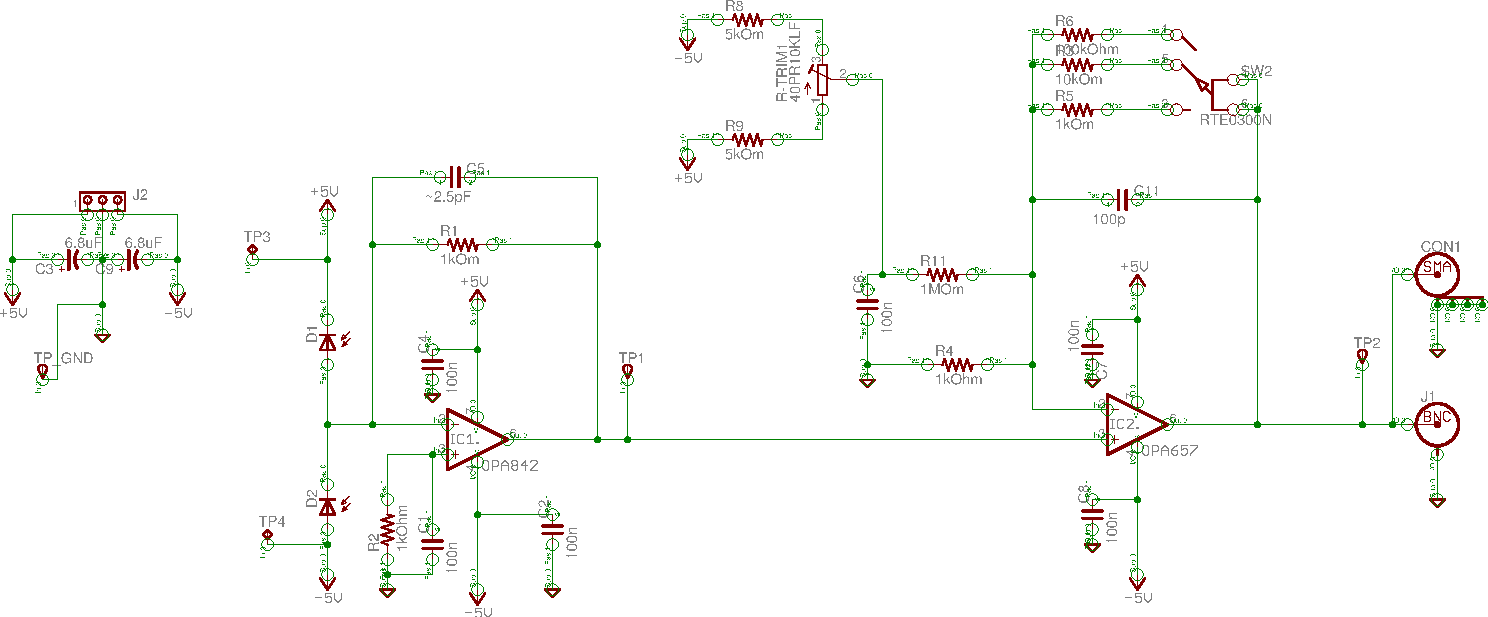
\includegraphics[width=0.9\textwidth]{./pics/bpd_v3_schematics.pdf}
  \end{column}
 \end{columns}

 \vskip .2in
 \begin{columns}[t]
  \begin{column}{.5\textwidth}
   Board layout
   \begin{figure}
   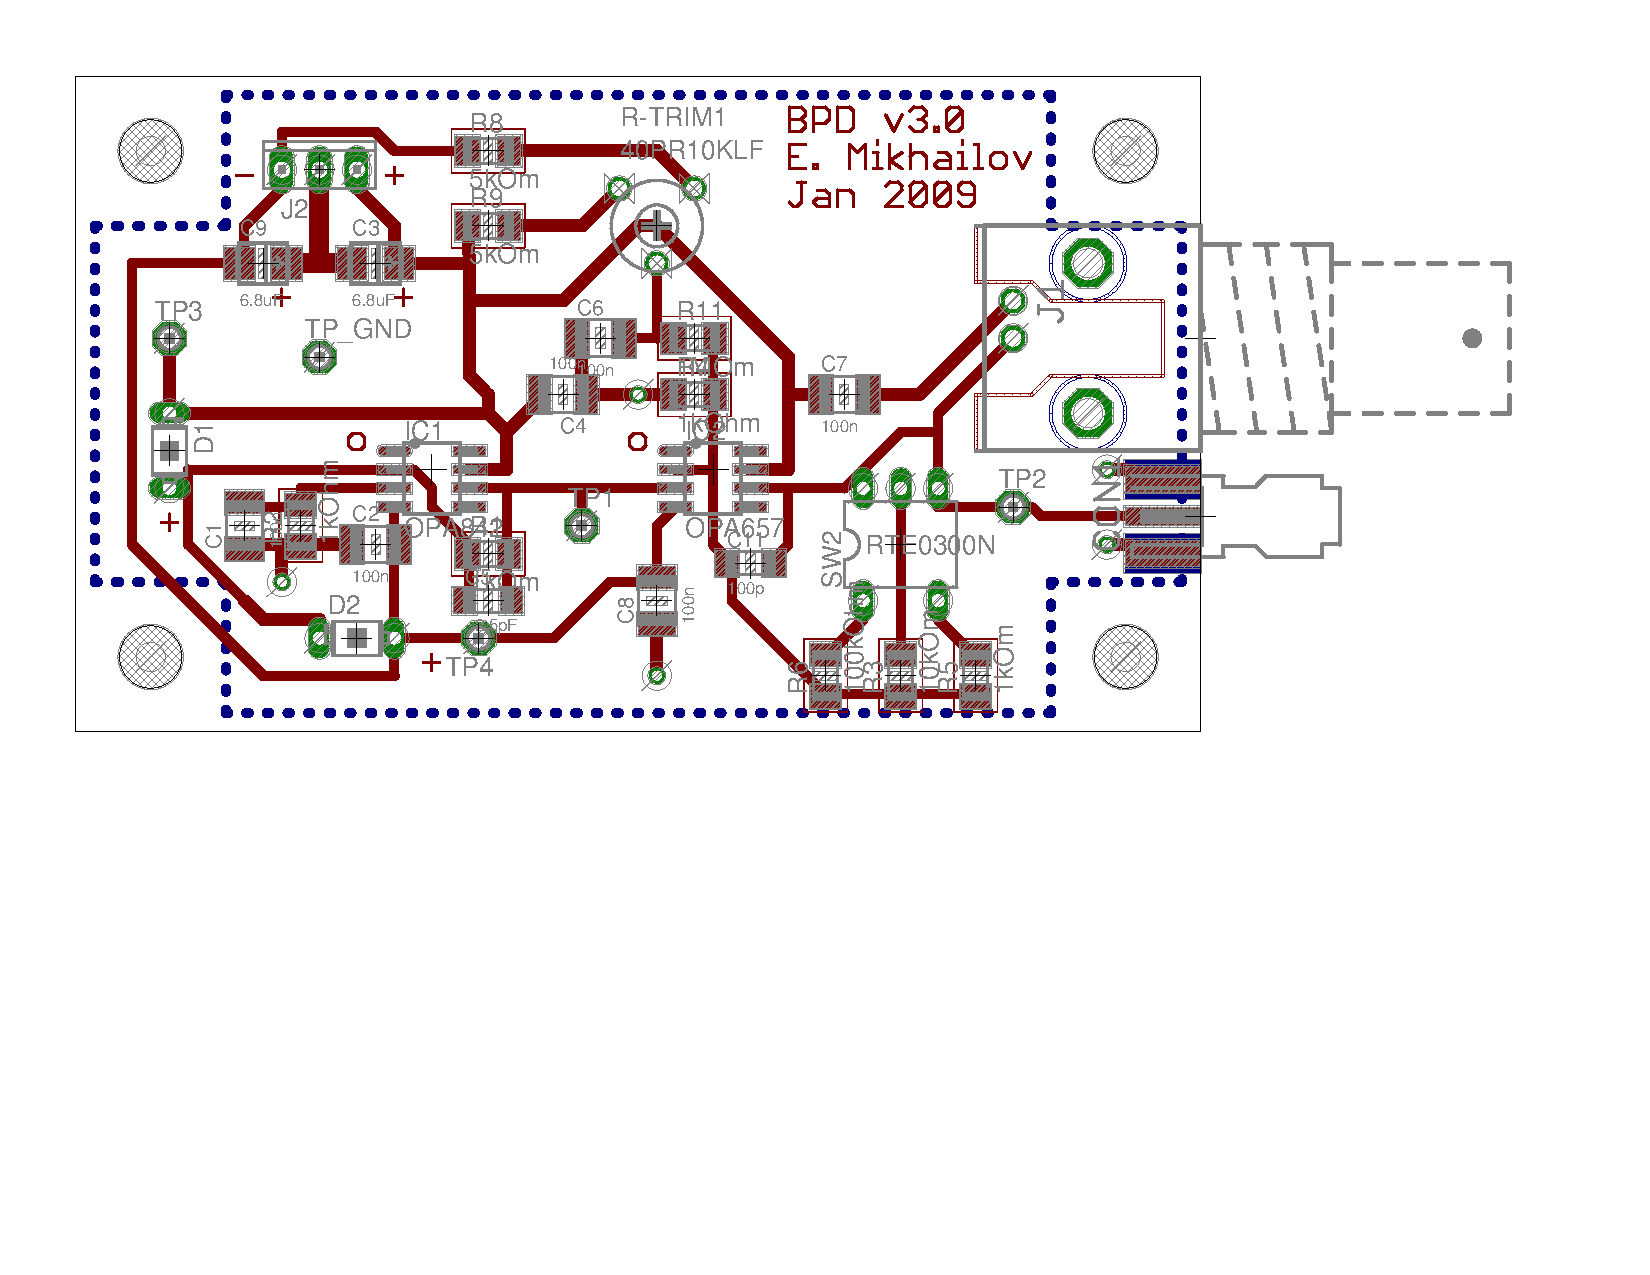
\includegraphics[angle=0,width=0.99\textwidth]{./pics/bpd_v3_board.pdf}
   \end{figure}
  \end{column}
  \begin{column}{.5\textwidth}
   Hardware
   \begin{figure}
   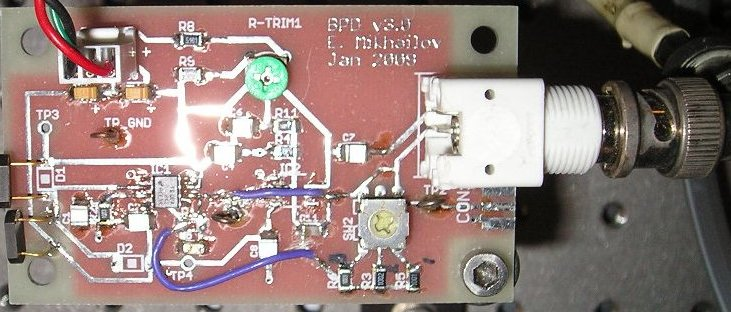
\includegraphics[angle=0,width=0.99\textwidth]{./pics/PDboard_finished}
   \end{figure}
  \end{column}
 \end{columns}
\end{frame}


\begin{frame}
\frametitle{Contact info}
{\bf Instructor: Wouter Deconinck}
\begin{itemize}
 \item Office: Small Hall 343D
 \item Lab: Small Hall 234
 \item Phone: 221-3539 (office)
 \item Email: \htmladdnormallink{wdeconinck@wm.edu}{mailto:wdeconinck@wm.edu}
 \item Office Hours: by appointment through \url{http://doodle.com/wdeconinck}.
\end{itemize}

{\bf T.A. lab book graders: Charlie Fancher, Drew Rotunno}

\end{frame}

\begin{frame}
\frametitle{Evaluations}
Your final grade for the course will be determined from the following grading weight distribution:

\begin{itemize}
\item Lab Book:   35\%
\item Design Exercises:  10\%
\item Quizzes:  5\%
\item Participation:  10\%  (\alert{being in class/lab is not enough})
\item Midterm:   20\%
\item Final:   20\%
\end{itemize}
\end{frame}


\begin{frame}
\frametitle{Lab books}
Your lab book is \alert{the primary record of your work and data}.  

\begin{itemize}
 \item What you did.
 \item How you did it (e.g. circuit diagrams).
 \item How you made measurements (which test equipment and how it was connected).
 \item Your data and enough information to tell us what that data is.
 \item What you observed (oscilloscope traces).
 \item Your calculations and analysis (including scratch work). 
 \item Plots (labeled axes).
 \item Answers to questions and justifications for your answers.
\end{itemize}

Once something is entered in your lab book it should never be modified, only amended by making a clear comment or by referring to a later page.
\end{frame}


\begin{frame}
\frametitle{Lab books}

\begin{block}{Neatness of Your Lab Books}
Diagrams, data, graphs, and other notes on separate pieces of paper should be
glued, taped, or stapled into the lab book.

\alert{If something falls out of the lab book during reading, shaking, transporting,
it is not the part of the lab book and will be discarded.}

The lab book will be graded primarily on completeness but to some extent also on neatness.
It should be clear and readable for the grader and yourself!
\end{block}

\begin{block}{Design Exercises}
Most labs will include a design exercise.
\alert{The designs must be prepared in your lab book prior to attending a lab}.
I will check preparation of the design exercise at the beginning of each lab.
\alert{An unprepared/incomplete design exercise will have at least 50\% penalty.}
\end{block}
\end{frame}


\begin{frame}
\frametitle{Due days}
\begin{block}{Lab Books}
Lab books are due by 9:00 pm on the next day after lab (i.e. Wednesday for the Tuesday section, Thursdays for the Wednesday section, and Fridays for the Thursday section) and will be returned by the next lab period.

Late lab books submission will have  points deducted. If you  know you will have a problem getting  the report on time please send me  an email as soon as you can to let me know about your situation.
\end{block}

\begin{block}{Illness}
Please notify the instructor if you are ill, so that arrangements can be made to make up missed labs.
\end{block}
\end{frame}


\begin{frame}
\frametitle{Tests and Exams}
\begin{block}{Pre-Lecture Quizzes}
Pre-lecture quizzes are \textbf{due by 10am} on the day of the lecture (on blackboard).  They will test that you have engaged with the readings, and will not include any difficult problems.
\end{block}

\begin{block}{Midterm exam}
There will a 1 hour midterm exam in lab the \textbf{week of March 2} (before spring break). There will be a shortened lab session after the midterm.
\end{block}

\begin{block}{Final exam}
There will be a final exam on \textbf{Monday May 4, 9:00 am--noon} (to be confirmed) covering all course materials.
\end{block}
\end{frame}


\begin{frame}
\frametitle{Grades table}
\begin{center}\begin{tabular}{|l|l|l|l|l|l|}
\hline \textbf{Grade} & \textbf{Score} & \textbf{Grade} &
\textbf{Score} & \textbf{Grade} & \textbf{Score} \\
\hline A- & 90-93 & A & 93-100 &    &       \\
\hline B- & 80-83 & B & 83-86  & B+ & 86-90 \\
\hline C- & 70-73 & C & 73-76  & C+ & 76-80 \\
\hline D- & 60-63 & D & 63-66  & D+ & 66-70 \\
\hline F  & $<$60 &   &        &    &       \\
\hline \end{tabular}\end{center}
\end{frame}


\begin{frame}
\frametitle{Calendar}
\url{http://blackboard.wm.edu}
\end{frame}

\section{DC Circuits Basics}
\begin{frame}
 \frametitle{Basic blocks}
 \begin{block} { Voltage (V)}
  Short for electrical potential difference\\
  Potential energy divided by charge ($V=E/Q$) \\
  Derived Unit: J/C \\  
  SI unit: V (Volt)
 \end{block}
 
 \begin{block} { Current (I)}
  Rate of flow of electric charge ($dQ/dt$)\\
  SI unit: A (Ampere)
 \end{block}

 \begin{block} {Power (P)}
  Energy per time (dE/dt) \\
  In electronics: $P=V I$ \\
  SI unit: W (Watt)
 \end{block}
\end{frame}

\begin{frame}
 \frametitle{Electrical resistance}
 \begin{block} { Resistance (R) }
 Different objects have different current passing through when the same voltage difference is applied.
 
 Which indicates: they have different
 electrical resistance.

 SI unit: $\Omega$ (Ohm)
 \end{block}

 \begin{block}{Ohm's law}
 \[I = \frac{V}{R} \]
 \end{block}
\end{frame}

\begin{frame}
 \frametitle{Resistors}
 \begin{columns}[t]
  \begin{column}{.3\textwidth}
   Standard leaded
   \begin{figure}
   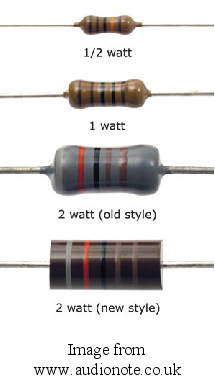
\includegraphics[width=0.85\textwidth]{./pics/resistors1.png}
   \end{figure}
  \end{column}
  \begin{column}{.3\textwidth}
   Power
   \begin{figure}
   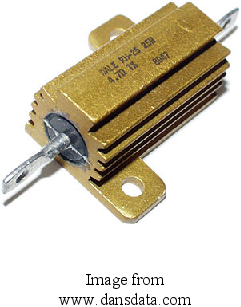
\includegraphics[width=0.85\textwidth]{./pics/resistors2.png}
   \end{figure}
  \end{column}
  \begin{column}{.3\textwidth}
   Surface mounted
   \begin{figure}
   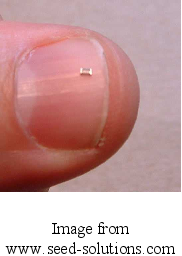
\includegraphics[width=0.85\textwidth]{./pics/resistors3.png}
   \end{figure}
  \end{column}
 \end{columns}
\end{frame}


\begin{frame}
 \frametitle{Resistor color code}
 \vskip -.1in
 \begin{figure}
  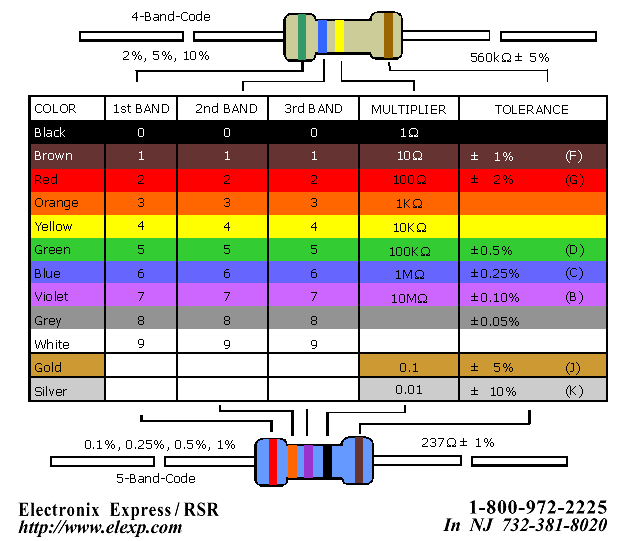
\includegraphics[width=0.8\textwidth]{./pics/clr_code.png}
 \end{figure}
\end{frame}

\begin{frame}
 \frametitle{Resistors usage} 
 \begin{itemize}
  \item current limiters
  \item fix voltage from a current source (exotic use)
  \item generate heat 
  \item fuse (non standard use)
  \item lowering the voltage of the source (i.e. voltage dividers)
 \end{itemize}
\end{frame}


\begin{frame}
 \frametitle{Combinations of resistors}
 \begin{block}{Series}
  \begin{equation*}
   R_{eq} = R_1 + R_2
  \end{equation*}
  \begin{itemize}
   \item Always $R_{eq} > R_1, R_2$
   \item If $R_1 \ll R_2$, then $R_{eq} \sim R_2$
  \end{itemize}
 \end{block}
 \begin{block}{Parallel}
  \begin{equation*}
   \frac{1}{R_{eq}} = \frac{1}{R_1} + \frac{1}{R_2} \quad \hbox{or} \quad R_{eq} = \frac{R_1 R_2}{R_1 + R_2}
  \end{equation*}
  \begin{itemize}
   \item Always $R_{eq} < R_1, R_2$
   \item If $R_1 \ll R_2$, then $R_{eq} \sim R_1$
  \end{itemize}
 \end{block}
\end{frame}


\section{Voltage divider}
\begin{frame}
 \frametitle{Unloaded voltage divider}
 \begin{columns}[c]
  \begin{column}{.3\textwidth}
   \begin{figure}
    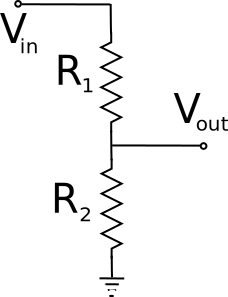
\includegraphics[height=2in]{./pics/unloaded_voltage_divider}
   \end{figure}
  \end{column}
  \begin{column}{.7\textwidth}
   \[ V_{out} = V_{in} \frac{R_2}{R_1+R_2} \]
  \end{column}
 \end{columns}
\end{frame}

\begin{frame}
 \frametitle{Loaded voltage divider}
 \begin{columns}[c]
  \begin{column}{.3\textwidth}
   \begin{figure}
    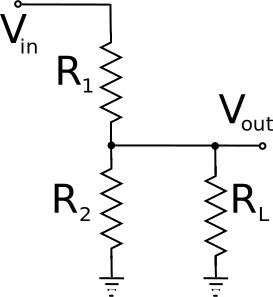
\includegraphics[height=2in]{./pics/loaded_voltage_divider}
   \end{figure}
  \end{column}
  \begin{column}{.7\textwidth}
   \[ V_{out,loaded} = V_{in} \frac{R_2}{R_1+R_2} \frac{R_L}{R_L + R_{1||2}} \]
   \[ V_{out,loaded} = V_{out,unloaded} \frac{R_L}{R_L + R_{1||2}} \]
  \end{column}
 \end{columns}
\end{frame}

\end{document}


\end{document}

\documentclass{article}

\usepackage{import}
\subimport{preamble/}{lab_preamble.tex}

%
% Ideas:
% - make one of the resistors in the voltage divider a potentiometer and let the students twiddle it to see how the output voltage changes
% - use this to then introduce a three terminal potentiometer as a voltage divider itself
%




\title{Lab 1: Voltage, Current, Resistance, and Power}


\begin{document}
\maketitle

\section{Overview}
Electrical circuit design depends first and foremost on understanding the basic quantities used for describing electricity: voltage, current, and power. In the simplest circuits these are related by Ohm's law. After defining and understanding these quantities, we will begin a discussion of network analysis and look at a few examples.

\subsection{Voltage}
\emph{Voltage} (measured in volts, V) is electrical potential difference between two points in a circuit. You measure a voltage by connecting the two terminals of a \emph{voltmeter} to the two points in your circuit. You must measure the voltage while your circuit is operating. If you have a good voltmeter, your measured voltage will be the same as the voltage was before you connected the voltmeter. A voltage decrease in the direction of current flow represents energy flowing out of the circuit (usually into heat). Voltage sources, such as batteries and power supplies, produce voltage increases along the direction of current
flow.

\subsection{Current}
\emph{Current} (measured in amperes or amps, A, which is equivalent to Coulombs/second) is measured at a single point in a circuit. It is the rate at which charge flows along the circuit. To measure a current with a \emph{current meter (or ammeter)} you must break the circuit at that point and connect each end to one of the terminals of the ammeter. Current can only flow in complete circuits. That's why a switch stops an electrical circuit: it breaks the circuit and interrupts the current flow.

\subsection{\boldmath$IV$ Characteristic}
We can completely characterize any element that has two terminals by its $IV$ characteristic (i.e. how much current flows through it when a given voltage is put across it). The $IV$ characteristic is given by the functions $I(V)$ or $V(I)$ and is frequently defined graphically.  

\subsection{Ground}
\emph{Ground} is the name given to the V = 0 reference point. This makes it easier to refer to voltages, since you can generally assume that the second point is ground if it is not explicitly stated. We will also use it to represent the implied completion of a circuit, even when we do not explicitly show a wire connection between different places in a circuit, since all ground connections are connected together.

\subsection{Resistance}
A \emph{resistor} is a two-terminal device that converts a voltage into a current or converts a current into a voltage. The current through a resistor is always related to the voltage drop across the resistor by Ohm's Law
\begin{equation}
V = IR
\end{equation}
where $R$ is the resistance (measured in Ohms, $\Omega$) This also means that a resistor generates heat when a current flows given by:
\begin{equation}
 P = IV = I^2 R = \frac{V^2}{R}.
\end{equation}
Each of these expressions give the same answer but one or the other will be easier to use, depending on what you know about the circuit ($I$ or $V$, or both). It may seem silly to have a device that just turns electrical energy into heat, but resistors actually perform many important roles:
\begin{itemize}
\item They turn electrical energy into heat. This can be useful if you want to make an electrical heater, or (more likely) a light bulb. Light is just a form of heat given off by a very hot source. Sometimes you must dissipate power somewhere. For example, if you want to deliver 100\,mA current at 12\,V to part of your circuit, but your power supply gives you 15\,V, then the extra power
\begin{equation}
300\,mW = (100\,mA) (15\,V - 12\,V) 
\end{equation}
must go somewhere. You dissipate it in a resistor rather than by heating your sensitive transistors.
\item If you have a voltage source and you want a specific amount of current then a resistor does the job. It converts a voltage difference between two points into a current flowing through the resistor. Sometimes, you will add a resistor in series in a circuit to prevent the power supply from delivering too much current in case you short the output lines together. This is called a \emph{current limiting resistor}.
\item If you have a current flowing and you want to convert it into a voltage then a resistor is again the solution. This might seem a little more far-fetched, because you may not be familiar with constant current sources. When we begin studying transistors we will find that they will behave as \emph{current sources}. So we will use a resistor on the output to convert the current into a voltage.
\end{itemize}
When we consider capacitors, in week three, we will generalize resistance for AC circuits by allowing for phase shifts. We will call this generalization to the complex plane \emph{impedance}. For this week we will assume resistance and impedance to mean the same thing.

\section{Network Analysis}
If you connect one power supply and lots of resistors together in a complicated network, then currents will flow through all the various elements so as to insure that charge is conserved, energy is conserved, and Ohm's Law is satisfied. Simultaneously satisfying all these conditions will give you exactly one solution. We will start with two resistors and then proceed to more complicated systems. Specifically, two resistors in series will draw the same current as an equivalent resistor with resistance. This is stated mathematically as:
\begin{equation}
R_S = R_1 + R_2
\end{equation}
Alternatively, two resistors in parallel will draw current equivalent a resistor with resistance
\begin{equation}
\frac{1}{R_\parallel} = \frac{1}{R_1} + \frac{1}{R_2} \quad \hbox{or} \quad R_\parallel = \frac{R_1 R_2}{R_1 + R_2}
\end{equation}
Note that the resistance of 2 resistors in parallel is always less than the smaller, but not less than half of that smaller resistance. If the two resistors differ by a large factor, then you can ignore the larger resistor. For example, a 1\,k\Ohm in parallel with 1\,M\Ohm is within 999\,\Ohm or very close to 1\,k\Ohm.

Standard resistors come in a few dozen difference ratings (more on this in lab). So in general one can get any particular value one wants. One can make up an equivalent resistor using a few resistors in series and parallel combinations to get a much larger range of options. In Design Exercise 1-1, we have you design a network to have a specific net resistance given a very limited set of resistances.

\subsection{Voltage Dividers}
\begin{figure}
\centering
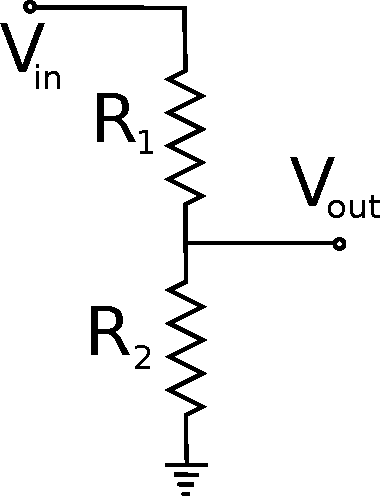
\includegraphics[height=0.2\textheight]{pics/unloaded_voltage_divider.pdf}
\caption{A voltage divider.}
\label{fig:unloaded_voltage_divider}
\end{figure}
By far the most useful thing you can do with two resistors is to make a \emph{voltage divider}, which is just two resistors in series. Voltage dividers are shown schematically in Figure~\ref{fig:unloaded_voltage_divider} in two slightly different but equivalent representations. It ``divides'' a total voltage into two parts with each part proportional to the resistance in that leg. So, if you know the starting voltage and the target voltage, then you can calculate the required ratio of the two resistors.
\begin{equation}
V_{out} = V_{in} \frac{R_2}{R_1 + R_2}
\end{equation}
In Design Exercise 1-2 you get to derive this relationship.

\subsection{Loaded Voltage Divider}
\begin{figure}
\centering
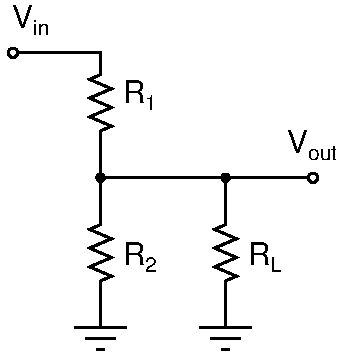
\includegraphics[height=0.2\textheight]{pics/loaded_voltage_divider.pdf}
\caption{A loaded voltage divider.}
\label{fig:loaded_voltage_divider}
\end{figure}
Of course, the way you will use $V_{out}$ from a voltage divider is to connect it to something, usually another resistor, as shown in Figure~\ref{fig:loaded_voltage_divider}. This then changes the equivalent resistance in the lower leg, and therefore changes the voltage across that leg!

In order to choose the actual resistor values, you have two competing concerns:
\begin{itemize}
\item low resistance makes the divider less sensitive to loading when you use the target voltage (i.e. ``stiffer''),
\item high resistance draws less current, and therefore uses less power.
\end{itemize}
We'll spend more time on this and formalize the considerations in the coming weeks. 

For now, let's just consider what happens to our voltage divider when we connect a load resistance ($R_L$) from its output to ground. In this case we can replace the $R_2$ from the expression for the unloaded divider with an equivalent resistance of $R_2$ and $R_L$ in parallel. This gives us a voltage across $R_L$ of:
\begin{eqnarray}
 V_{out,loaded} & = & V_{in} \frac{R_{2 \parallel L}}{R_1 + R_{2\parallel L}} \\
 & = & V_{out,unloaded} \frac{R_L}{R_L + R_{1||2}}
\end{eqnarray}
where $R_{2 \parallel L}$ is the equivalent resistance of $R_2$ and $R_L$ in parallel, $R_{1 \parallel 2}$ is the equivalent resistance of $R_1$ and $R_2$ in parallel, and $V_{out,unloaded}$ is the output voltage of the unloaded voltage divider. From the last expression it is clear that the loaded voltage is always less than the unloaded voltage. The smaller the load the larger the difference between loaded and unloaded, while large load resisters do not affect the output significantly. 

So, if you want to ensure that you do not affect the output of a device, you would like to have the input of your device to look like a large resistor and the output look (in this case $R_{1\parallel 2}$) look like a small resistance. Next week we'll show that this is a general conclusion and more formally define these concepts.


\pagebreak

\section{Lab 1: Design Exercises}

\begin{enumerate}
\item Design Exercise 1-1: Use only 10\,k\Ohm resistors to create a network with an equivalent resistance of 6.67\,k\Ohm. What is the minimum number of required resistors?
\item Design Exercise 1-2: Use network analysis and Ohm's Law to derive a formula for $V_{out}$­ for an unloaded voltage divider.
\item Design Exercise 1-3: Assuming that $R_1$, $R_2$ and $R_L$ are 10\,k\Ohm resistors and $V_{in}$ is 10\,V, compute $V_{out}$ for both a loaded voltage divider and an unloaded voltage divider­. How much does the output voltage change when it is loaded?
\end{enumerate}

\section{Lab 1: Voltage, Current, Resistance and Power}

\emph{Your notebooks must be complete, understandable, and address all activities, design exercises, observations, and questions noted in the laboratory's procedures. Remember to use your notebook as a laboratory journal and record your data, design calculations, notes and scratch work. Make sure to write a conclusion for each exercise and each week.} 

\begin{enumerate}
\item Measure the resistances of a few resistors with an ohmmeter and see how well they match their specified values. Are they within specifications, based on their tolerance bands?
\item Construct the resistor network you designed in Design Exercise 1-1. Check to see that the total resistance agrees with your calculation. Put 10\,V into your device and use an ammeter to see if it draws the expected current. How much power is being consumed, and how would one measure it?
\item Make a voltage divider from 1--100\,k\Ohm resistors and apply input voltages in the range of 2\,V--15\,V. Measure the input voltages and the current of this device. Be sure to sketch your experimental setup in your lab notebook! Plot your measurements with the voltage on the vertical axis and the current on the horizontal axis. The equivalent or input resistance of your voltage divider is the slope of the curve. Relate this to the resistors you used to construct the voltage divider.
\item Make your voltage divider from Design Exercise 1-3. Apply constant input voltage equal to 10\,V and measure the output voltage and output current for a variety of load resistances in the range from 100\,\Ohm to 100\,k\Ohm (use at least 10 different load resistors). Note how the output voltage changes and compare your results to your calculations. Do the results make sense?
\item Learn to start your oscilloscope and perform some basic tests. Feel free to consult the scope's manual to help you with the details as needed.
\begin{enumerate}
\item Select default configuration.
\item Connect a $10\times$ probe (look for a hardware switch on the probe) to channel 1, connect the ground to the scopes test ground, and connect the probe tip to the calibration test point on the front of the scope. You should see a square wave appear with a 1\,kHz frequency and 5\,V amplitude. 
\item Adjust the trim screw on the probe until the edges of the square wave are true (instead of rolling over or overshooting).
\item Verify the edges with a $1\times$ probe setting as well. 
\item Test the probe's calibration (i.e. do you get 1\,kHz and a 5\,V amplitude?). Record the result.
\item Zoom in and out on the signal and play with some of the measurements available to you on the scope (i.e. period, frequency, $V_{pp}$).
\end{enumerate}
\end{enumerate}

\end{document}

\documentclass{article}


% This file is a solution template for:
% 1 inch margins
\usepackage{fullpage}

\usepackage{booktabs}
\usepackage{longtable}

\usepackage{hyperref}
\usepackage{graphicx}
\usepackage{multicol}
\usepackage{subcaption}

% Add ability to resume enumeration environments with /begin{enumerate}[resume]
\usepackage{enumitem}

\usepackage{pgf}
\usepackage{tikz}
\usepackage{bodegraph}
\usepackage{circuitikz}
\usetikzlibrary{calc}
\usetikzlibrary{trees}
\usetikzlibrary{arrows}
\usetikzlibrary{shapes}
\usetikzlibrary{fadings}
\usetikzlibrary{positioning}
\usetikzlibrary{intersections}


\usepackage[english]{babel}
\usepackage[latin1]{inputenc}
\usepackage[T1]{fontenc}
% Or whatever. Note that the encoding and the font should match. If T1 does not look nice, try deleting the line with the fontenc.


\usepackage{listings}

\usepackage{amsmath}


\usepackage{xspace}
\newcommand{\Ohm}{$\Omega$\xspace}



\title{Voltage, Current, Resistance, and Power}

\begin{document}
\maketitle

\section{Lab 1: Voltage, Current, Resistance and Power}

\subsection*{General comments}

\begin{itemize}
\item Make one of the resistors in the voltage divider a potentiometer and let the students twiddle it to see how the output voltage changes.
\item Use this to then introduce a three terminal potentiometer as a voltage divider itself.
\end{itemize}

\end{document}


\chapter{Lab 2: Voltage, Current, Resistance, and Power}
\documentclass[beamer]{standalone}
\usepackage{import}

\usepackage{pgfpages}
\pgfpagesuselayout{4 on 1}[letterpaper,border shrink=5mm,landscape]

\import{preamble/}{beamer_presentation_preamble.tex}

\begin{document}
\date{Lecture 02}
\import{lecture02/}{slides02.tex}
\end{document}

\documentclass{article}

\usepackage{import}
\subimport{preamble/}{lab_preamble.tex}


\title{Kirchhoff's Laws and Th\'{e}venin's Theorem}


\begin{document}
\maketitle

In this course we will be using a variety of mathematical and conceptual models to describe the electrical components and circuits that we will encounter. Ohm's Law was the first such model. In this chapter we will consolidate some of the concepts from last week into a generic model of a linear device known as a \emph{Th\'{e}venin equivalent circuit} (with input impedance, output impedance, and internal voltage).

The Th\'{e}venin equivalents will also be generalized and used to describe properties of signals. A \emph{signal} will be described not only by its \emph{voltage} but also by the \emph{output impedance} of the device that produced or transported it. The concept of the \emph{impedance of a signal} will be used extensively through this course as we discover various methods to transform the properties of a signal.

This week we will also examine network analysis in a complete framework known as Kirchhoff's Laws.  These rules will allow us to analyze the properties of any combination of resistors and power supplies. 

\section{Kirchhoff's Laws}
If you connect lots of power supplies and resistors together in a complicated network, then currents will flow through all the various elements so as to insure that charge is conserved, energy is conserved, and Ohm's Law is satisfied for each resistor. Simultaneously satisfying all these conditions will give you exactly one solution. The method for writing down equations to represent these conservation laws is called Kirchhoff's Laws. To explore these laws, we will consider the sample circuit shown in Figure~\ref{fig:circuit} on the right.

\begin{figure}
 \begin{center}
  \begin{circuitikz}
   \draw (-2,2) to[R,l=$R_1$,i=$I_1$,-*] (0,2);
   \draw (2,2) to[R,l=$R_2$,i=$I_2$,-*] (0,2);
   \draw (0,0) to[short,*-] (2,0) to[battery1,l=$V_2$] (2,2);
   \draw (0,0) to[short,*-] (-2,0) to[battery1,l=$V_1$] (-2,2);
   \draw (0,2) to[R,l=$R_3$,i=$I_3$] (0,0) to (0,-0.1) node[ground]{};
  \end{circuitikz}
 \end{center}
 \caption{A circuit with two power supplies and three resistors. A choice of current directions is indicated.}
 \label{fig:circuit}
\end{figure}

\subsection{Kirchhoff's Point Law}
\emph{Kirchhoff's Point Law} says that all of the current that flows into a junction must come out of the junction. This means that charge is conserved---none falls out of the circuit or pools in any location. This concept is illustrated for the top junction in the example circuit (see Figure~\ref{fig:circuit}). In this case, we have
\begin{equation}
 I_1 + I_2 - I_3 = 0.
\end{equation}
Note the sign conventions. We say that a current is positive if we define it to flow into the junction and negative if we define it to flow out the junction.

\subsection{Kirchhoff's Loop Law}
\emph{Kirchhoff's Loop Law} says that if you sum the voltage drops around any closed loop in a circuit the total must be zero. Since the voltage drops represent the energy per unit charge, this means that all the energy which comes out of the circuit (in heating resistors, for example) must come from some power sources (such as power supplies). This is just conservation of energy. 

The sign conventions are that the voltage increases across a power supply and decreases across a resistor in the direction of current flow. The direction of current flow should be the same as the one defined for the Point Law. In our example circuit there are three loops that could be considered. From these three loops, we obtain the three following relationships:
\begin{eqnarray}
 0 & = & V_1 - I_1 R_1 + I_2 R_2 - V_2 \\
 0 & = & V_1 - I_1 R_1 - I_3 R_3 \\
 0 & = & V_2 - I_2 R_2 - I_3 R_3
\end{eqnarray}
Any two of these relationships (since all three are not independent) and the point relationship can be used to solve for the current in each resistor and hence the power in each resistor. 

It can be a real nightmare to solve more complicated networks and we will develop models and methods to avoid solving complicated networks wherever we can. We will usually do this by making one part of a circuit relatively independent of another part. Our most common use of Kirchhoff's Laws will usually be to say that $V = I R$ and apply the simple relationships for resistors connected in series or parallel. In the next section we will begin to explore how this is possible. 

\section{Th\'{e}venin Equivalents}
The Th\'{e}venin equivalents are models to describe the input and output properties of a device. We will assume the input of a device looks like a resistor with the other end connected to ground.  We will assume that an output looks like an ideal voltage source followed by a resistor. Both of these are shown in Figure~\ref{fig:thevenin}, below. Note that for this week's discussion the term resistance and impedance are treated as synonymous. 

\begin{figure}
 \begin{center}
  \begin{circuitikz}
   \draw (-2,2) to[R,l=$R_{in}$,o-] (0,2) to (0,0) node[ground]{};
  \end{circuitikz}
  \quad
  \begin{circuitikz}
   \draw (-2,0) node[ground]{} to[battery1,l=$V_{Th}$] (-2,2) to[R,l=$R_{Th}$,-o] (0,2);
  \end{circuitikz}
 \end{center}
 \caption{The Th\'{e}venin equivalent circuit for an input device (left), and the Th\'{e}venin equivalent circuit for a voltage source (right).}
 \label{fig:thevenin}
\end{figure}

One can determine the input impedance ($R_{in}$) by simply applying a voltage to the input, measuring the current flowing into the device, and applying Ohm's Law.

Given any electrical device with two output terminals (we will assume one is called ground) there are a number of you might do to try to determine its properties:
\begin{enumerate}
\item Measure the voltage across the terminals.
\item Attach a resistor across the terminals and then measure the voltage.
\item Change the resistor and measure the voltage again, repeat.
\end{enumerate}
Clearly, these are all variations on one simple measurement. What is the minimum number of measurements you must do to characterize this black box completely? Th\'{e}venin's answer is just two! 

\subsection{Th\'{e}venin's Theorem}
Any linear (i.e. Ohmic) system with two terminals can be completely characterized as an ideal voltage source ($V_{Th}$ or Th\'{e}venin voltage) in series with one resistor ($R_{Th}$ or Th\'{e}venin resistance, and also sometimes called internal resistance). No matter what resistance ($R_L$) you connect across the two terminals, it just forms a voltage divider, as shown in Figure~\ref{fig:voltage_divider} on the right, and so the voltage across that load resistor is given by: 
\begin{equation}
V_L = V_{Th} \left( \frac{R_L}{R_{Th} + R_L} \right)
\end{equation}

\begin{figure}
 \begin{center}
  \begin{circuitikz}
   \draw (-2,0) node[ground]{} to[battery1,l=$V_{Th}$] (-2,2) to[R,l=$R_{Th}$] (0,2) to[short] (1,2) to[R,l=$R_L$,i=$I_L$,v=$V_L$] (1,0) node[ground]{};
  \end{circuitikz}
 \end{center}
 \caption{A voltage source connected to a load can be treated as voltage divider.}
 \label{fig:voltage_divider}
\end{figure}

A special case is when there isn't any load applied (i.e. option 1 above, where $R_L = \infty$) then the output is simply $V_{Th}$. From the results of these two measurements we can solve for $R_{Th}$.

\subsection{Voltage Divider as a Th\'{e}venin Device}
Let's consider what happens to our voltage divider from last week when we connect a load resistance to its output. From last week we computed the output of a loaded voltage divider was given by:
\begin{equation}
V_L = V_{in} \frac{R_2}{R_1 + R_2} \frac{R_L}{R_{1\parallel 2} + R_L}
\end{equation}
If we equate factors from in this relationship with the ones in the previous section, we can see that for a loaded voltage divider produces Th\'{e}venin equivalents of 
\begin{eqnarray}
 V_{Th} & = & V_{in} \frac{R_2}{R_1 + R_2} \\
 R_{Th} & = & R_{1 \parallel 2} = \frac{R_1 R_2}{R_1 + R_2}
\end{eqnarray}
The relationship for $V_{Th}$ makes sense.  It is simply the unloaded output voltage as describe in the previous section. The output impedance is simply the parallel equivalent of the two resistors on the voltage divider. 

\subsection{Designing a Stiff Voltage Divider}
A stiff output implies that the output voltage stays relatively close to its Th\'{e}venin, or unloaded, voltage when a load is implied. A rule of thumb for designing a stiff voltage source is that the output should not deviate by more than about 10\% when loaded. From the relationships in the previous section, we can see that this implies that the load resistance must be more than a factor of 10 larger than the output impedance (in the voltage divider case $R_{Th} = R_{1\parallel 2}$). We can think of this at a \emph{Rule of 10}. We will usually design it so that R1 itself is smaller than the expected load by a factor of 10. 

\subsection{Generalization and Application of the Rule of 10 and Notable Exceptions}
Since we are going to design and construct some very complicated circuits this year, we need to be able to focus on parts of circuits, which we will call sub-circuits. For example, we will often build amplifiers in three stages. The basic idea is to always insure that the downstream elements do not load the upstream elements. (1) The first stage will be a ``buffer'' amplifier that takes a signal and amplifies the current but not the voltage. This will allow us to connect it to the next part of the amplifier without changing (i.e. loading) the characteristics of whatever generated the signal. The second stage will be a voltage amplifier that amplifies a signal's voltage to whatever level we need. The final stage will be another buffer amplifier that again amplifies the current so that we will not load our voltage amplifier when we use its output. 

This gains us two major advantages: We will never have a large number of interdependent simultaneous equations to solve, and our circuits will work under a wide range of differing operational conditions.
Here is the general procedure: 
\begin{itemize}
\item Any sub-circuit can be modeled, using Th\'{e}venin's Theorem, as an ideal voltage source ($V_{Th}$) in series with a resistance ($R_{Th}$).
\item When we connect this to the next sub-circuit we can represent that by a load resistance ($R_L$) thus making a voltage divider. 
\item We can keep our equations simple, so that we need not employ the full Kirchhoff's Laws formalism, simply by following a ``factor of 10'' rule. 
\end{itemize}
In summary, anything we design to produce a reliable voltage should have $R_{Th}$ smaller $R_L$ by least a factor of 10. That is, we do not want the voltage to change significantly when the sub-circuit is connected to subsequent parts of the circuit.

\subsection{Constant Voltage Sources}
The most common sub-circuit we will use will supply a voltage to a later part of a circuit. It may be a power supply to power all the other sub-circuits, or it may be a biasing network to keep a transistor in its normal operating region. For these type sub-circuits, we want $V_L$ to be relatively independent of $R_L$, so this means $R_L > 10 R_{Th}$.

\subsection{Constant Current Sources}
We will later see that transistors are current amplifiers. This means that we will often want to drive an amplifier with a current source. A current source can also be modeled as ideal voltage source in series with an $R_{Th}$. Again, the complete circuit will look like an ideal voltage source driving a voltage divider, but we want the current through $R_L$ to be relatively independent of $R_L$. This means we want the same current as when we remove $R_L$ and just connect (or ``short'') the two leads together. By applying the same logic above this implies that we want $R_L < 10 R_{Th}$ for a stiff current source.

\subsection{Impedance Matching}
There are two cases when we require $R_L = R_{Th}$, which we will call ``impedance matching''. If you want the most efficient transfer of power to your load, then you must choose $R_L = R_{Th}$. By the most efficient transfer, we mean that 
\begin{equation}
 P_L = I^2 R_L = \left( \frac{V_{Th}}{R_L + R_{Th}} \right)^2 R_L
\end{equation}
will have its largest value when $R_L = R_{Th}$. Of course this will severely load the source, dropping the output voltage by exactly a factor of two. This may, however, be fine in simple circuits -- like lighting a light-bulb or driving an audio speaker. 

The second case is when you have very fast signals traveling along transmission cables such as the BNC cables that we often use to connect laboratory equipment. Then, we will want to prevent reflections at our connections, since these could give rise to phony signals. Then we will want to choose $R_L = R_{Th}$, even though it will decrease the amplitude of the signal. We often accomplish this matching by attaching a 50\,\Ohm \emph{terminator} to the end of our BNC cable to ensue that the impedance is matched.


\pagebreak

\section{Lab 2: Design Exercises}

\begin{enumerate}
\item \label{exercise:wheatstone} Use Kirchhoff's laws to determine the resistance of the Wheatstone bridge depicted in the circuit in Figure~\ref{fig:wheatstone}.  \emph{Hint:} complete the circuit with a voltage source and feel free to use a computer to solve the resulting system of equations in the currents and voltages.  Another approach could be to use a ``Delta-Wye'' transformation\ldots
\item \label{exercise:voltage_divider} Find a relationship between $V_L$, $I_L$, and $R_{Th}$ that does not depend on $R_L$ in the Th\'{e}venin equivalent circuit of Figure~\ref{fig:voltage_divider}.
\item How would you measure the Th\'{e}venin resistance and voltage of a power supply?
\item Prove that the power transfer from a power supply with Th\'{e}venin resistance, $R_{Th}$, to a load resistor, $R_L$, is maximum when $R_L = R_{Th}$.
\end{enumerate}

\begin{figure}
 \begin{center}
  \begin{circuitikz}
   \draw (-2,0) to[short] (-1.5,0) to[R,l=$R_1$] (0,1.5) to[R,l=$R_2$] (1.5,0) to[short] (2,0);
   \draw (-1.5,0) to[R,l=$R_3$] (0,-1.5) to[R,l=$R_4$] (1.5,0);
   \draw (0,1.5) to[R,l=$R_5$] (0,-1.5);
  \end{circuitikz}
 \end{center}
 \caption{A Wheatstone bridge circuit.}
 \label{fig:wheatstone}
\end{figure}


\section{Lab 2: Kirchhoff, Th\'{e}venin, and Impedance Matching}

\begin{enumerate}
\item Construct a Wheatstone bridge from 5 resistors in the 1--10 k\Ohm range. Measure its resistance at a few voltages (i.e. measure current and voltage). What is its resistance? Does it agree with your calculation from design exercise \ref{exercise:wheatstone}? 
\item Construct a voltage divider similar to the one you made last week for lab exercises 3 and 4. Set $V_{in}$ to 10 V and measure $V_{Th}$ and $R_{Th}$ seen by a load resistor---you will not be able to measure $R_{Th}$ directly, so you will have to come up with a method for doing so (hint: the result of design exercise \ref{exercise:voltage_divider} can be usefully adapted to make a measurement). Do the measured $V_{Th}$ and $R_{Th}$ agree with what you expect from your calculations?
\item Use your voltage divider setup from part 2. Determine experimentally the load resistance which results in the maximum output power out of the voltage divider.
\item Set the breadboard power supply to 3\,V and determine $V_{Th}$ and $R_{Th}$ of the breadboard power supply for this setting. Before doing your measurements, you should list the potential difficulties of such an experiment (including the uncertainty on the difference of two nearly equal measured voltages). You should also consult with the instructors before attempting it: do not let $I_{out}$ exceed 1.5\,A.  \textbf{Do not, under any circumstances, connect an ammeter or a load resistor less than 1\,\Ohm directly to power supply.}  Comment on the engineering of the power supply. 
\end{enumerate}

\end{document}

\documentclass{article}


% This file is a solution template for:
% 1 inch margins
\usepackage{fullpage}

\usepackage{booktabs}
\usepackage{longtable}

\usepackage{hyperref}
\usepackage{graphicx}
\usepackage{multicol}
\usepackage{subcaption}

% Add ability to resume enumeration environments with /begin{enumerate}[resume]
\usepackage{enumitem}

\usepackage{pgf}
\usepackage{tikz}
\usepackage{bodegraph}
\usepackage{circuitikz}
\usetikzlibrary{calc}
\usetikzlibrary{trees}
\usetikzlibrary{arrows}
\usetikzlibrary{shapes}
\usetikzlibrary{fadings}
\usetikzlibrary{positioning}
\usetikzlibrary{intersections}


\usepackage[english]{babel}
\usepackage[latin1]{inputenc}
\usepackage[T1]{fontenc}
% Or whatever. Note that the encoding and the font should match. If T1 does not look nice, try deleting the line with the fontenc.


\usepackage{listings}

\usepackage{amsmath}


\usepackage{xspace}
\newcommand{\Ohm}{$\Omega$\xspace}



\title{Kirchhoff's Laws and Th\'{e}venin's Theorem}


\begin{document}
\maketitle

\section{Lab 2: Kirchhoff, Th\'{e}venin, and Impedance Matching}

\subsection*{General comments}


\end{document}


\chapter{Lab 3: Voltage, Current, Resistance, and Power}
\documentclass[handout]{beamer}
\usepackage{pgfpages}

\pgfpagesuselayout{4 on 1}[letterpaper,border shrink=5mm]

% This file is a solution template for:
%\includeonlyframes{draft}
% This file is a solution template for:

% below to make handout 
%\usepackage{pgfpages}
%\pgfpagesuselayout{4 on 1}[letterpaper,landscape, border shrink=5mm]

% This file is a solution template for:

% - Talk at a conference/colloquium.
% - Talk length is about 20min.
% - Style is ornate.

\usepackage{standalone}
\usepackage{import}

\usepackage{bookmark}

\usepackage{pgf}
\usepackage{tikz}
\usepackage{bodegraph}
\usepackage{circuitikz}
\usetikzlibrary{calc,arrows,shapes,trees,fadings,positioning,intersections}

\tikzstyle{block} = [draw, fill=blue!20, rectangle, 
    minimum height=3em, minimum width=6em]
\tikzstyle{sum} = [draw, fill=blue!20, circle, node distance=1cm]
\tikzstyle{input} = [coordinate]
\tikzstyle{output} = [coordinate]
\tikzstyle{pinstyle} = [pin edge={to-,thin,black}]

% Copyright 2004 by Till Tantau <tantau..
%
% In principle, this file can be redistributed and/or modified under
% the terms of the GNU Public License, version 2.
%
% However, this file is supposed to be a template to be modified
% for your own needs. For this reason, if you use this file as a
% template and not specifically distribute it as part of a another
% package/program, I grant the extra permission to freely copy and
% modify this file as you see fit and even to delete this copyright
% notice. 

\mode<presentation>
{
  \usetheme{Madrid}  % for short upt to 20min presentation
  \setbeamercovered{transparent}

  \setbeamertemplate{footline}%
  {%
    \leavevmode%
    \hbox{%
    \begin{beamercolorbox}[wd=.5\paperwidth,ht=2.25ex,dp=1ex,left]{}%
      \hspace*{1ex} \insertlogo
    \end{beamercolorbox}%
    \begin{beamercolorbox}[wd=.5\paperwidth,ht=2.25ex,dp=1ex,right]{}%
      \insertframenumber{} \hspace*{1ex}
    \end{beamercolorbox}}%
    \vskip0pt%
  }

  % No navigation symbols
  \setbeamertemplate{navigation symbols}{}
}


\usepackage[english]{babel}
% or whatever

\usepackage[latin1]{inputenc}
% or whatever

\usepackage{times}
\usepackage[T1]{fontenc}
% Or whatever. Note that the encoding and the font should match. If T1
% does not look nice, try deleting the line with the fontenc.

\usepackage{listings}
\usepackage{amsmath}



%\setbeamercovered{transparent}
\setbeamercovered{invisible}



%\subtitle
%{Include Only If Paper Has a Subtitle}

\subimport{./}{authors.tex}


%{Wouter Deconinck\inst{1} \and S.~Another\inst{1}}
% - Give the names in the same order as the appear in the paper.
% - Use the \inst{?} command only if the authors have different
%   affiliation.

% If you have a file called "university-logo-filename.xxx", where xxx
% is a graphic format that can be processed by latex or pdflatex,
% resp., then you can add a logo as 

%remember extension must be ommited
\pgfdeclareimage[height=1cm]{cc-by-sa}{styles/CC-BY-SA_icon.png}
%\logo{\pgfuseimage{cc-by-sa}}

\institute[CC BY-SA] % (optional, but mostly needed)
{
  \pgfuseimage{cc-by-sa}
}
% - Use the \inst command only if there are several affiliations.
% - Keep it simple, no one is interested in your street address.

% If you wish to uncover everything in a step-wise fashion, uncomment
% the following command: 
%\beamerdefaultoverlayspecification{<+->}

%
\providecommand{\fixme}[1]{%
  { \em ---! FixMe #1 !---}
}
%
\providecommand{\hide}[1]{%
}
%
\providecommand{\mat}[1]{% matlab code
{\color{blue}\texttt{#1}}%
}
%
\providecommand{\mstr}[1]{% matlab code string
{\color{magenta}#1}%
}

% {{{ listing color schem definitions
\definecolor{listcommentcolor}{rgb}{0.0,0.4,0} %dark green
%\definecolor{listbg}{rgb}{0.67,0.90,0.64} %pale green
\definecolor{listbg}{rgb}{0.90,0.90,0.90} %kight grey
\lstset{backgroundcolor=\color{listbg}}
\lstset{commentstyle=\color{listcommentcolor}}
\lstset{keywordstyle=\color{blue}}
\lstset{stringstyle=\color{magenta}}
\lstset{language=matlab}
\lstset{tabsize=2}
\lstset{showstringspaces=false}
\lstset{basicstyle = \ttfamily}
% }}}



\begin{document}

\date{Lecture 03}
\documentclass[beamer]{standalone}
\begin{document}

\title[Electronics 1] % (optional, use only with long paper titles)
{
	Alternating-Current Circuits
}

\begin{frame} 
  \titlepage
\end{frame}

\hide{
\begin{frame}
  \frametitle{Outline}
  \tableofcontents
  % You might wish to add the option [pausesections]
\end{frame}
}

\begin{frame}{Complex Number}
 \begin{block}{Out with $i$, in with $j$}
  Since $i$ will be reserved for currents, so complex numbers will be indicated with $j$ instead, with
  \begin{equation}
   j^2 = -1
  \end{equation}
 \end{block}
 \begin{block}{Properties of complex numbers, also covered in Physics 301}
  \begin{itemize}
   \item $\frac{1}{j} = \frac{j}{j^2} = \frac{j}{-1} = -j$
   \item $j = e^{j \pi/2}$ so $\frac{1}{j} = j^{-1} = e^{-j \pi/2}$
   \item $z = |z| e^{j \phi} = |z| \cos\phi + j |z| \sin\phi$
  \end{itemize}
 \end{block}
 \begin{block}{Physical meaning of complex numbers}
  We will use complex impedance $Z$ and complex gain $G(\omega)$ to indicate a phase shift of $\phi$
 \end{block}
\end{frame}

\section{Complex Impedances}
\begin{frame}
 \frametitle{Alternating-Current Signals}
 \begin{block}{Exponential notation}
  Consider voltage and current as real part of complex exponential:
  \begin{eqnarray*}
   v(t) & = & v_0 \cos(\omega t + \phi_v) = v_0 Re (e^{j (\omega t + \phi_v)}) \\
   i(t) & = & i_0 \cos(\omega t + \phi_i) = i_0 Re (e^{j (\omega t + \phi_i)})
  \end{eqnarray*}
  Now do all calculations in complex numbers.
 \end{block}
 \begin{block}{Resistors and Ohm's law: no phase difference}
  Resistance is given by
  \begin{equation*}
   R = \frac{v(t)}{i(t)} = \frac{v_0}{i_0} e^{j (\phi_v - \phi_i)}
  \end{equation*}
  but because $i(t)$ is always in phase with $v(t)$, we always have $(\phi_v - \phi_i) = 0$.
 \end{block}
\end{frame}

\begin{frame}
 \frametitle{Alternating-Current Signals}
 \begin{block}{Components with phase difference}
  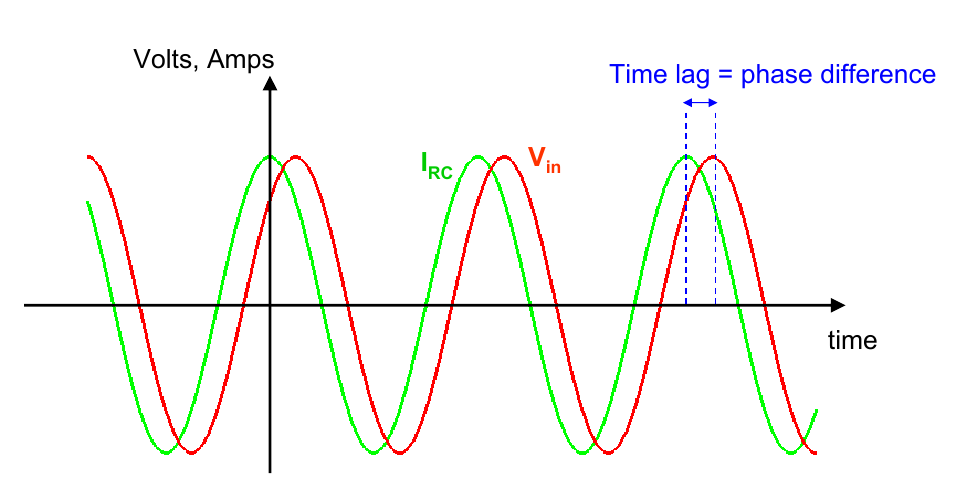
\includegraphics[width=\textwidth]{pics/Phase_difference} \\
  CIVIL: in capacitor I before V; V before I in inductor
 \end{block}
\end{frame}


\begin{frame}[t]
 \frametitle{Complex Impedances}
 \begin{block}{Impedance $Z$ of common components}
  \begin{center}
   \begin{tabular}{c|c|l|l}
    resistor & R & \\
    capacitor & $\frac{1}{j\omega C}$ & open for $\omega \to 0$ & short for $\omega \to \infty$ \\
    inductor & $j\omega L$ & short for $\omega \to 0$ & open for $\omega \to \infty$ \\
   \end{tabular}
  \end{center}
 \end{block}
 \only<2>{
 \begin{block}{Example: inductor}
  Start from differential equation describing inductor
  \begin{eqnarray*}
   v(t) & = & L \frac{d}{dt} i(t) = L \frac{d}{dt} Re(i_0 e^{j(\omega t + \phi_i)}) \\
        & = & Re(j \omega L i_0 e^{j(\omega t + \phi_i)})
  \end{eqnarray*}
  The impedance is then
  \begin{equation*}
   Z(\omega) = \frac{v(t)}{i(t)} = \frac{j \omega L i_0 e^{j(\omega t + \phi_i)}}{i_0 e^{j(\omega t + \phi_i)}} = j \omega L
  \end{equation*}
 \end{block}
 }
 \begin{block}{Impedances in series and in parallel}<3>
  \begin{itemize}
   \item In series: $Z = Z_1 + Z_2$
   \item In parallel: $\frac{1}{Z} = \frac{1}{Z_1} + \frac{1}{Z_2}$
   \item Because $Z \sim \frac{1}{C}$ this works for capacitors.
  \end{itemize}
 \end{block}
\end{frame}

\begin{frame}
 \frametitle{Complex Impedances}
 \begin{block}{Example: RLC circuit}
  \begin{center}
   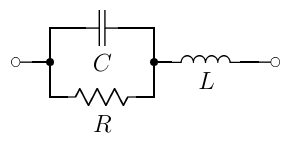
\includegraphics[width=0.4\textwidth]{pics/RLC_circuit}
  \end{center}
  \only<1>{What is the equivalent impedance $Z_{eq}$?}
 \end{block}
 \begin{block}<2->{Equivalent impedance}
  \begin{equation*}
   Z_{eq} = \frac{R}{j \omega R C + 1} + j \omega L
  \end{equation*}
  \only<2>{What are the limits for small and large $\omega$?}
 \end{block}
 \begin{block}<3->{Limits for small and large $\omega$}
  \begin{itemize}
   \item $\omega \approx 0$ (DC limit): $Z_{eq} \approx R$
   \item $\omega \to \infty$ (high frequency limit): $Z_{eq} \approx j\omega L$
  \end{itemize}
 \end{block}
\end{frame}


\section{Power Dissipation and Root-Mean-Square}
\begin{frame}
 \frametitle{Power Dissipation}
 \begin{block}{Power dissipation in resistor: root mean square}
  Dissipated power in a resistor is 
  \begin{equation*}
   P_{avg} = R \frac{1}{T} \int_{t=0}^T i(t)^2 dt = R I_{RMS}^2 = V_{RMS} I_{RMS}
  \end{equation*}
 \end{block}
 \begin{block}{Power dissipation in general impedance}
  \begin{equation*}
   P_{avg} = \frac{1}{T} \int_{t=0}^T v(t) \cdot i(t) dt
  \end{equation*}
  \begin{itemize}
   \item In phase (like a resistor): $P_{avg} = \frac{1}{2} v_0 i_0 = V_{RMS} I_{RMS}$
   \item $90^\circ$ out of phase (like a capacitor or inductor): $P_{avg} = 0$
   \item Anything in between: $Z = R + j X$, with reactance $X$
  \end{itemize}
 \end{block}
\end{frame}
\begin{frame}
 \frametitle{Power Dissipation}
 \begin{block}{Power factor}
  \begin{itemize}
   \item Dissipated power only depends on $R$
   \item Power company still has to generate $|Z|$
   \item Keep ratio ($\sim$ power factor) close to 1 with large capacitor banks
  \end{itemize}
 \end{block}
 \begin{center}
  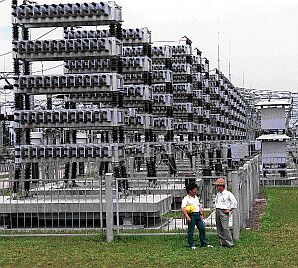
\includegraphics[width=0.45\textwidth]{pics/capacitor_bank}
 \end{center}
\end{frame}


\section{Transformers}
\begin{frame}
 \frametitle{Transformers}
 \begin{columns}
  \begin{column}{0.4\textwidth}
   \includegraphics<1>[width=\textwidth]{pics/transformers_prime}
   \includegraphics<2>[width=\textwidth]{pics/transformers} \\
   \only<2>{Flux $\Phi = \mu N_1 i_1(t) A$, where $A$ cross-sectional area, $N_1$ windings}
  \end{column}
  \begin{column}{0.6\textwidth}
   \begin{block}{Magnetic flux conserved}
    \begin{itemize}
     \item EMF $\mathcal{E}$ by $v_1(t)$ and $v_2(t)$ must be equal, so
      \begin{equation*}
       v_2 = \frac{N_2}{N_1} v_1
      \end{equation*}
     \item Energy conservation requires that $P_1 = P_2 = i(t) v(t)$, so
      \begin{equation*}
       i_2 = \frac{N_1}{N_2} i_1
      \end{equation*}
     \item If we connect a load $Z_L$ across terminals 2, $v_2 = i_2 Z_L$, and then
      \begin{equation*}
       Z_{eq} = \frac{v_1}{i_1} = \left(\frac{N_1}{N_2}\right)^2 Z_L
      \end{equation*}
    \end{itemize}
   \end{block}
  \end{column}
 \end{columns}
\end{frame}



\section{Gain of a Circuit}
\begin{frame}[t]
 \frametitle{Gain of a Circuit}
 \begin{block}{Input/output voltage}
  \begin{columns}
   \begin{column}{0.0\textwidth}
   \end{column}
   \begin{column}{0.35\textwidth}
    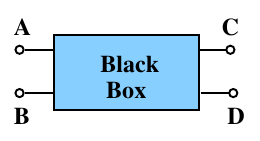
\includegraphics[width=\textwidth]{pics/Black_box}
   \end{column}
   \begin{column}{0.65\textwidth}
    \begin{itemize}
     \item Gain $G$ is $V_{CD} / V_{AB}$
     \item If $V_{CD}$ is 1.5\,V when $V_{AB}$ is 0.5\,V, \\ then the gain is 3.
    \end{itemize}
   \end{column}
  \end{columns}
 \end{block}
 \begin{block}{Gain of a DC voltage divider}
  \begin{columns}
   \begin{column}{0.0\textwidth}
   \end{column}
   \begin{column}{0.2\textwidth}
    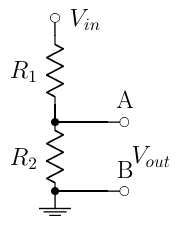
\includegraphics[width=\textwidth]{pics/Voltage_divider}
   \end{column}
   \begin{column}{0.8\textwidth}
    \begin{itemize}
     \item Voltage divider with two resistors: \\ input $V_{AB}$ is $V_{in}$, output $V_{CD}$ is $V_{out}$
     \item Gain $G$ is $V_{out} / V_{in} = \frac{R_2}{R_1 + R_2}$
     \item Now extend this concept to alternating-current signals\ldots
    \end{itemize}
   \end{column}
  \end{columns}
 \end{block}
\end{frame}

\begin{frame}[t]
 \frametitle{Gain of a Circuit}
 \begin{block}{Gain of a AC voltage divider}
  \begin{columns}
   \begin{column}{0.0\textwidth}
   \end{column}
   \begin{column}{0.5\textwidth}
    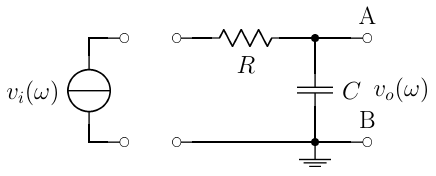
\includegraphics[width=\textwidth]{pics/RC_filter}
   \end{column}
   \begin{column}{0.5\textwidth}
    \begin{itemize}
     \item Gain $G(\omega)$ is now $v_o(\omega) / v_i(\omega) = \frac{Z_2(\omega)}{Z_1(\omega) + Z_2(\omega)}$
     \item $G(\omega)$ depends on frequency!
     \item $G(\omega)$ is a complex number!
    \end{itemize}
   \end{column}
  \end{columns}
 \end{block}
 \begin{columns}[t]
  \begin{column}{0.5\textwidth}
   \begin{block}{Impedances of RC-circuit}
    \begin{eqnarray*}
     Z_1 & = & R \\
     Z_2 & = & \frac{1}{j\omega C}
    \end{eqnarray*}
   \end{block}
  \end{column}
  \begin{column}{0.0\textwidth}
  \end{column}
  \begin{column}{0.5\textwidth}
   \begin{block}{Gain of this RC-circuit}
    \begin{eqnarray*}
     G(\omega) & = & \frac{1}{j\omega C} \frac{1}{R +\frac{1}{j\omega C}} \\
               & = & \frac{1}{1 + j\omega R C}
    \end{eqnarray*}
   \end{block}
  \end{column}
 \end{columns}
\end{frame}

\begin{frame}
 \frametitle{Gain of a Circuit}
 \begin{block}{Limits of gain in an RC-circuit}
  \begin{columns}
   \begin{column}{0.0\textwidth}
   \end{column}
   \begin{column}{0.5\textwidth}
    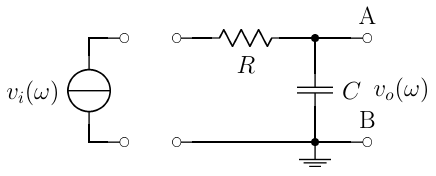
\includegraphics[width=\textwidth]{pics/RC_filter}
   \end{column}
   \begin{column}{0.5\textwidth}
    \begin{equation*}
     G(\omega) = \frac{1}{1 + j\omega R C}
    \end{equation*}
   \end{column}
  \end{columns}
  \begin{itemize}
   \item Low frequency $\omega \ll \frac{1}{RC}$: $G(\omega) \approx 1$ (DC limit)
   \item High frequency $\omega \gg \frac{1}{RC}$: $G(\omega) \approx \frac{1}{j\omega R C} \approx 0$
  \end{itemize}
 \end{block}
 \only<1>{
 \begin{block}{Bode plots}
  \begin{center}
   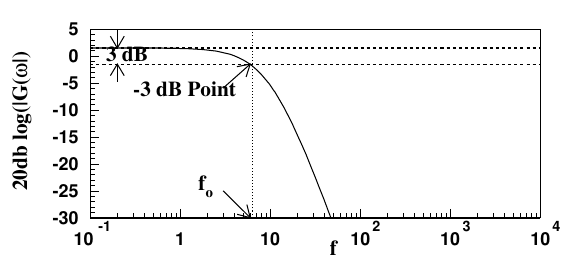
\includegraphics[width=0.4\textwidth]{pics/Bode_plot}
  \end{center}
 \end{block}
 }
 \only<2>{
 \begin{block}{Exercise: Swapping $R$ and $C$}
  \begin{itemize}
   \item How will the gain change when $R$ and $C$ are swapped?
   \item How will the Bode plot change?
  \end{itemize}
 \end{block}
 }
\end{frame}

\section{Power dissipation}
\begin{frame}
\frametitle{Power dissipation}
	Recall that power dissipated by element is
	\[P=V I\] where $V$ and $I$ are real.

	Since we use a  substitute \\
	$V\cos(\omega t) \to V e^{j \omega t}$ 
	and  $I\cos(\omega t) \to I e^{j \omega t}$,  \\
	we need to write
	\alert{
	\[P=Re(V) Re(I)\]
	}
	Recall the Ohm's law
	\[ V=Z I\]
\end{frame}

\begin{frame}
\frametitle{Power dissipation by a reactive element}
	\begin{theorem} 
		{\bf Average power dissipated by a reactive element (C or L) is 0} \\
		Lets use as example an inductor. \\
		\vskip -.1in
		\[Z_L=i \omega L = e^{i \frac{\pi}{2}} \omega L,
		 I_L= I_p e^{ i \omega t} \]
		\[V_L=Z_L I_L = e^{i \frac{\pi}{2}} \omega L I_L
		= \omega L I_p e^{ i (\omega t + \frac{\pi}{2} ) }  \]
		\[ Re(I_L)=I_p \cos(\omega t),  Re(V_L)= - \omega I_p L \sin(\omega t) \]
		Thus average power dissipated by the inductor
		\[P=\int^T_0 Re(I_L) Re(V_L) dt
		= - \int^T_0 I_p \cos(\omega t) \omega I_p L \sin(\omega t) dt \]
		\[P
		= - \omega I_p^2 L \int^T_0 \cos(\omega t) \sin(\omega t) dt 
		= \omega I_p^2 L \int^T_0 \frac{1}{2} \sin(2 \omega t) dt = 0\]
	\end{theorem}
\end{frame}

\end{document}


\end{document}

\documentclass{article}


% This file is a solution template for:
% 1 inch margins
\usepackage{fullpage}

\usepackage{booktabs}
\usepackage{longtable}

\usepackage{hyperref}
\usepackage{graphicx}
\usepackage{multicol}
\usepackage{subcaption}

% Add ability to resume enumeration environments with /begin{enumerate}[resume]
\usepackage{enumitem}

\usepackage{pgf}
\usepackage{tikz}
\usepackage{bodegraph}
\usepackage{circuitikz}
\usetikzlibrary{calc}
\usetikzlibrary{trees}
\usetikzlibrary{arrows}
\usetikzlibrary{shapes}
\usetikzlibrary{fadings}
\usetikzlibrary{positioning}
\usetikzlibrary{intersections}


\usepackage[english]{babel}
\usepackage[latin1]{inputenc}
\usepackage[T1]{fontenc}
% Or whatever. Note that the encoding and the font should match. If T1 does not look nice, try deleting the line with the fontenc.


\usepackage{listings}

\usepackage{amsmath}


\usepackage{xspace}
\newcommand{\Ohm}{$\Omega$\xspace}



\title{Capacitors, Inductors, and Complex Impedance}


\begin{document}
\maketitle

In this chapter we introduce the concept of complex resistance, or \emph{impedance}, by studying two reactive circuit elements, the \emph{capacitor} and the \emph{inductor}. We will study capacitors and inductors using differential equations and Fourier analysis and from these derive their impedance. Capacitors and inductors are used primarily in circuits involving time-dependent voltages and currents, such as AC circuits.

\section{AC Voltages and circuits}
Most electronic circuits involve time-dependent voltages and currents. An important class of time-dependent signal is the sinusoidal voltage (or current), also known as an AC signal (Alternating Current). \emph{Kirchhoff's laws and Ohm's law still apply (they always apply), but one must be careful to differentiate between time-averaged and instantaneous quantities.}

An AC voltage (or signal) is of the form:
\begin{equation}
v(t) = V_0 \cos\omega t
\end{equation}
where $\omega$ is the angular frequency, $V_0$ is the amplitude of the waveform or the \emph{peak voltage} and $t$ is the time. The angular frequency is related to the frequency $f$ by $\omega = 2 \pi f$, and the period $T$ is related to the frequency by $T = \frac{1}{f}$. Other useful voltages are also commonly defined. They include the \emph{peak-to-peak voltage} ($V_{pp}$) which is twice the amplitude $V_0$, and the RMS voltage ($V_{RMS}$) which is $V_{RMS} = V_0 / \sqrt{2}$. The average power dissipated in a resistive AC device is computed using RMS quantities:
\begin{equation}
P = I_{RMS} V_{RMS} = \frac{1}{2} I_0 V_0.
\end{equation}
This is important enough that voltmeters and ammeters in AC mode actually return the RMS values for current and voltage.

While most real world signals are not sinusoidal, AC signals are still used extensively to characterize circuits through the technique of Fourier analysis.

\subsection{Fourier Analysis}
One convenient way to characterize the rate of change of a function is to write the true function as a linear combination of a set of functions that have particularly easy characteristics to deal with analytically. In this case we can consider the trigonometric functions. It turns out that we can write any function as an integral of the form
\begin{equation}
v(t) = \int v(\omega) \cos \left( \omega t + \phi(\omega) \right) d\omega
\end{equation}
where $v(\omega)$ and $\phi(\omega)$ are functions of the frequency $\omega$. This process is called Fourier analysis, and it means that any function can be written as an integral of simple sinusoidal functions. In the case of a periodic waveform this integral becomes a sum over all the harmonics of the period (i.e. all the integer multiplicative frequencies of the period).
\begin{equation}
v(t) = \sum_n A_n \cos (n\omega t + \phi_n).
\end{equation}
An implication of this mathematical fact is that \emph{if we can figure out what happens when we put pure sinusoidal voltages into a linear circuit, then we will know everything about its operation even for arbitrary input voltages.}

\subsection{Complex Notation}
In complex notation we replace our sinusoidal functions by exponentials to make the calculus and bookkeeping easier still. Then we can include both phase and magnitude
information. We'll define 
\begin{equation}
e^{j\phi} = \cos\phi + j\sin\phi,
\end{equation}
where $j^2 = -1$.

The general procedure for using this notation is:
\begin{enumerate}
\item Change your problem into complex algebra, i.e. replace $\cos\omega t$ with $e^{j \omega t}$.
\item Solve the problem.
\item Take the real part of the solution as your answer at the end.
\end{enumerate}


\section{Capacitors}
One of the most basic rules of electronics is that circuits must be complete for currents to flow. This week, we will introduce an exception to that rule.

The capacitor is actually a small break in a circuit. Try measuring the resistance of a capacitor, you will find that it is an open circuit. However, at the inside ends of the capacitor's lead, it has little plates that act as charge reservoirs where it can store charge. For short times, you do not notice that the break is there. Negative charge initially flows in to one side and out from out the other side just as if the two leads were connected. For fast signals, the capacitor ``looks'' like a short-circuit. But after a while the capacitor's reservoirs fill, the current stops, and we notice that there really is a break in the circuit.

For slow signals, a capacitor ``looks'' like an open circuit. What is fast, and what is slow? It depends on the capacitor and the rest of the circuit. This week, you will learn how to determine fast and slow for yourselves.

Capacitors serve three major roles in electrical circuits (although all three are just variations of one basic idea):
\begin{itemize}
\item Charge integrators;
\item High or low frequency filters;
\item DC isolators.
\end{itemize}

In order to perform these functions analytically, we will need to introduce a number of new concepts and some significant mathematical formalism. In this process we will also develop a number of new concepts in analyzing electronic circuits.

\subsection{Capacitance}
A capacitor is a device for storing charge and electrical energy. It consists of two parallel conducting plates and some non-conducting material between the plates, as shown in Figure~\ref{fig:capacitor}. When voltage is applied positive charge collects on one plate and negative charge collects on the other plane. Since they are attracted to each other this is a stable state until the voltage is changed again.

A capacitor's charge capacity or capacitance ($C$) is defined as:
\begin{equation}
 Q = C V
\end{equation}
which relates the charge stored in the capacitor ($Q$) to the voltage across its leads ($V$). Capacitance is measured in Farads (F). A Farad is a very large unit and most applications use $\mu$F, nF, or pF sized devices. Many electronics components have small parasitic capacitances due to their leads and design.

The capacitor also stores energy in the electric field generated by the charges on its two plates. The potential energy stored in a capacitor with voltage $V$ on it is
\begin{equation}
 E = \frac{1}{2} C V^2
\end{equation}
We usually speak in terms of current when we analyze a circuit. By noting that the current is the rate of change of charge, we can rewrite the definition of capacitance in terms of the current as:
\begin{eqnarray}
v & = & \frac{q}{C} = \frac{1}{C} \int i dt \\
i & = & C \frac{dv}{dt} = C \dot{v}
\end{eqnarray}
This shows that we can integrate a function $i(t)$ just by monitoring the voltage as the current charges up a capacitor, or we can differentiate a function $v(t)$ by putting it across a capacitor, and monitoring the current flow when the voltage changes.

\begin{figure}
\begin{center}
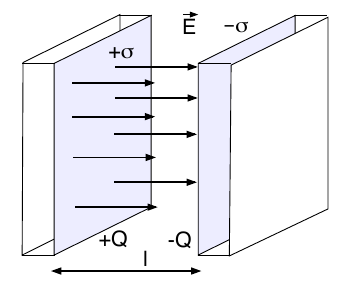
\includegraphics[width=0.4\textwidth]{pics/capacitor}
\end{center}
\caption{ A capacitor consist of two parallel plates which store equal and opposite amounts of charge.}
\label{fig:capacitor}
\end{figure}

\subsection{A Simple RC Circuit}

We will start by looking in detail at the simplest capacitive circuit, which is shown in Figure~\ref{fig:RC_circuit}. An RC circuit is made by simply putting a resistor and a capacitor together as a voltage divider. We will put the resistor in first, so we can connect the capacitor to ground.

By applying Kirchhoff's Laws to this circuit, we can see that:
\begin{itemize}
\item The same current flows through both the resistor and the capacitor, and
\item The sum of the voltage drops across the two elements equal the input voltage.
\end{itemize}
This can be put into a formula in the following equation:
\begin{equation}
v_{in} = i R + \frac{1}{C} \int i dt
\end{equation}
which can also be written as
\begin{equation}
\frac{v_{in}}{R} = i + \frac{1}{RC} \int i dt
\end{equation}
We can also put this into the form of a differential equation in the following way:
\begin{eqnarray}
\frac{dv_{in}}{dt} & = & R \frac{di}{dt} + \frac{i}{C}  \nonumber \\
C \dot{v}_{in} & = & R C \dot{i} + i
\label{eqn:RC_diffeqn}
\end{eqnarray}
These equations show that times are measured in units of $RC$, and that what you see depends on how quickly things change during one $RC$ time interval.

If the current changes quickly, then most of the voltage will show up across the resistor, while the voltage across the capacitor slowly charges up as it integrates the current. If the voltage changes slowly, then most of the voltage shows up across the capacitor as it charges. Since this usually requires a small current, the voltage across the resistor stays small.

But, what happens at intermediate times? To determine this quantitatively we will have to develop some more sophisticated mathematical techniques.

\subsection{Solutions to $RC$ Circuit}
Rather than produce the general solution, we will concentrate on two special cases that are particularly useful. The first will be for a constant voltage and the second will be a sinusoidal input.

\begin{figure}
 \begin{center}
  \begin{circuitikz}
   \draw (-2,0) node[ground]{} to[battery1,l=$v_{in}$] (-2,2) to[R,l=$R$] (0,2) to[C,l=$C$] (0,0) node[ground]{};
   \draw (0,2) to[short,-o] (1,2) node[right]{$v_{out}$};
  \end{circuitikz}
 \end{center}
 \caption{A simple RC circuit which integrates current.}
 \label{fig:RC_circuit}
\end{figure}

To study a constant supply voltage on an RC circuit, we set the left side of equation~\ref{eqn:RC_diffeqn} equal to a constant voltage. Then we have a simple homogeneous differential equation with the simple solution for the current of a decaying exponential,
\begin{equation}
 i = I_0 e^{-t/RC}
\end{equation}
which will account for any initial conditions. After a time of a few RC time periods, this solution will have decayed away to the supply voltage.

And now let us consider the other solution. In the prior section, we argued that if we can understand the $RC$ circuit's behavior for sinusoidal input we can deal with any arbitrary input. Therefore, this is the important one.

Let's look at our simple $RC$ circuit and suppose that we apply (or drive) a simple sine wave into the input:
\begin{equation}
v_{in} = V_0 \cos \omega t
\label{eqn:RC_voltage_cos}
\end{equation}
In complex notation, this means that we will set the drive voltage to
\begin{equation}
v_{in} = \Re \left(V_0 e^{j \omega t}\right)
\label{eqn:RC_voltage_exp}
\end{equation}
and we just have to remember to take the real part at the end of our calculation.

If we put this drive voltage into the differential equation \ref{eqn:RC_diffeqn}, then it becomes a relatively simple inhomogeneous differential equation:
\begin{equation}
C \frac{dv_{in}}{dt} = j \omega C V_0 e^{j \omega t} = R C \frac{di}{dt} + i.
\end{equation}
This is relatively simple because it shows up so often in physics that you might as well memorize the solution or at least the way to get the solution. Note that mathematically it looks just like a driven harmonic oscillator.

We can obtain the solution by using the standard recipe for first order linear differential equations. We start by rewriting equation as
\begin{equation}
\frac{di}{dt} + \frac{1}{R C} I = j \omega \frac{1}{R} V_0 e^{j \omega t}
\end{equation}
which we then multiply by $e^{t/RC}$ to obtain
\begin{equation}
e^{t/RC} \frac{di}{dt} + e^{t/RC} \frac{1}{R C} i = j \omega \frac{1}{R} V_0 e^{j \omega + \frac{1}{RC} t}.
\end{equation}

The left hand-side of this equality can be rewritten under the form of a total derivative (multiplication rule) so that we now have
\begin{equation}
\frac{d}{dt}\left[ i(t) e^{\left(t/RC\right)}\right] = \frac{j\omega V_0}{R} e^{\left( j\omega t + t/RC \right)}.
\end{equation}
This equation is easily integrable and can be rewritten as
\begin{equation}
i(t) e^{\left(t/RC\right)} = \frac{j\omega V_0}{R} \int e^{\left(j\omega t + t/RC\right)} dt.
\end{equation}
The integral is straightforward and yields the following expression:
\begin{equation}
i(t) = \frac{j\omega V_0}{R} \frac{1}{\frac{1}{RC} + j\omega} e^{\left(j\omega t\right)} + \hbox{constant} \cdot e^{\left( -t/RC \right)}.
\end{equation}
The first term represents the ``steady state'' oscillatory behavior of the driven circuit, while the second term describes the transient behavior of the current after switching on the driving voltage. Since we are only interested in the long-term behavior of the circuit, we neglect the second term and concentrate on the first. After a little bit of algebra, we can rewrite the steady-state current as
\begin{equation}
i(t) = \frac{j\omega V_0}{R} \frac{1}{\frac{1}{RC} + j\omega} e^{\left(j\omega t\right)} = \frac{\omega V_0 C}{\sqrt{1 + (\omega RC)^2}} \frac{\omega RC + j}{\sqrt{1 + (\omega RC)^2}} e^{\left(j\omega t\right)}.
\end{equation}
The second fraction can be interpreted as a phase term with $\tan\phi = \frac{1}{\omega RC}$, so that the expression for the current becomes
\begin{equation}
i(t) = I_0 e^{\left(j\omega t + \phi\right)}
\label{eqn:current_in_RC_circuit}
\end{equation}
with
\begin{equation}
I_0 = \frac{\omega V_0 C}{\sqrt{1 + \left(\omega RC\right)^2}} = \frac{V_0}{R} \cos\phi.
\end{equation}
The real solution of this simple RC circuit can be obtained by taking the real part of equation~\ref{eqn:current_in_RC_circuit}, and is left as an exercise to the reader.

The solution of the simple RC circuit appears to be rather complicated and involved, however it simplifies considerably when we plug equation~\ref{eqn:current_in_RC_circuit} back in to the original integral equation from Kirchhoff's loop law (equation~\ref{eqn:RC_diffeqn}). After integrating the exponential and a little bit of algebra, we obtain
\begin{equation}
v_{in}(t;\omega) = i(t) R + i(t) \frac{1}{j\omega C}
\end{equation}
This remarkably simple expression looks a lot like the standard Kirchhoff's loop law for resistors, except that the capacitor term behaves with a frequency dependent ``imaginary'' resistance.

\subsection{RC Impedance}
We will obtain the same solution as the one we obtained for the original voltage divider, as long as we assign an imaginary, frequency dependent, resistance to the capacitor. The ``imaginary'' part just means that it will produce a $\pi/2$ phase shift between the voltage and the current for a sinusoidal input. We will call this impedance
\begin{equation}
Z_C = \frac{1}{j \omega C}
\end{equation}

Now, the solution for an RC divider becomes somewhat simplified. We can compute the total current flowing through the circuit as
\begin{equation}
i = \frac{v_{in}}{Z_{tot}} = \frac{v_{in}}{R + Z_C} = \frac{V_0 e^{j\omega t}}{R + \frac{1}{j\omega C}} = \frac{j\omega C V_0 e^{j\omega t}}{1 + j\omega RC} = \frac{V_0}{R} \frac{j\omega RC e^{j\omega t}}{1 + j\omega RC} = \frac{V_0}{R} e^{j\omega t}  \cos\phi.
\end{equation}
The voltage across an element is just this current times the element's impedance. For the
voltage drop across the resistor it is largely the same as before:
\begin{equation}
v_R = i R = V_0 \cos\phi e^{j\left(\omega t + \phi\right)}
\end{equation}
For the capacitor, we get the following voltage drop:
\begin{eqnarray}
v_C = i Z_C = \frac{I}{j\omega C} & = & \frac{V_0 \cos\phi e^{j\left(\omega t + \phi\right)}}{j\omega RC} = -j V_0 \sin\phi e^{j\left(\omega t + \phi\right)} \\
& = & V_0 \frac{\cos\phi}{\omega RC} e^{j\left(\omega t + \phi + \pi/2\right)} = V_0 \sin\phi e^{j\left(\omega t + \phi + \pi/2\right)}.
\end{eqnarray}
If everything is correctly calculated then the sum of the voltage drops across the two elements should be equal to the input voltage. Let's try it:
\begin{equation}
v_R + v_C = V_0 \left( \cos\phi - j\sin\phi \right) e^{j\left(\omega t + \phi\right)} = V_0 e^{-j\phi} e^{j\left(\omega t + \phi\right)} = V_0 e^{j\omega t}.
\end{equation}
Remember, you get the actual waveforms by taking the real parts of these complex solutions. Therefore
\begin{eqnarray}
v_R & = & V_0 \cos\phi \cos(\omega t + \phi) \\
v_C & = & V_0 \sin\phi \cos(\omega t + \phi - \pi/2) = - V_0 \sin\phi \sin(\omega t + \phi)
\end{eqnarray}
This looks complicated, but the limits of high frequency and low frequency are easy to remember. At high frequencies ($\phi \to 0$), the capacitor is like a short, and all the voltage shows up across the resistor. At low frequencies ($\phi \to \pi/2$), the capacitor is like an open circuit, and all the voltage shows up across the capacitor.
If you consider the leading terms for the elements with the small voltages, you find that
\begin{eqnarray}
v_C & = & V_0 \frac{1 - j\omega RC}{1 + (\omega RC)^2} \to -\frac{j}{\omega} \frac{V_0}{RC} \quad \hbox{as}~\omega \to \infty, \\
v_R & = & V_0 \frac{\omega RC \left(1 + j\omega RC\right)}{1 + (\omega RC)^2} \to j\omega RC V_0 \quad \hbox{as}~\omega \to 0.
\end{eqnarray}
Thus, at high frequency, the voltage across the capacitor is the integral of the input voltage, while at low frequency the voltage across the resistor is the derivative of the input voltage. 

This says that as long as all the important frequencies are high, the capacitor will integrate the input voltage. If all the important frequencies are small, the resistor will differentiate the voltage. If there are intermediate frequencies, or a mixture of some high and some low frequencies, the result will not be so simple but it can be determined from the voltage divider algebra using complex notation.

We finish by noting that the voltage on the capacitor is always $-\pi/2$ out of phase with the voltage on the resistor.

\section{Inductors}

\begin{figure}
\begin{center}
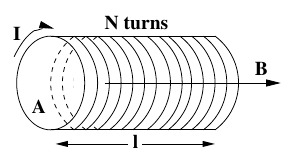
\includegraphics[width=0.5\textwidth]{pics/inductor}
\end{center}
\caption{An inductor consists of a coiled wire, also called a solenoid. The arrow $B$ represent the magnetic field generated by the current $I$ in the inductor.}
\label{fig:inductor}
\end{figure}

An inductors is a coil of wire, or solenoid, which can be used to store energy in the magnetic field that it generates (see Figure~\ref{fig:inductor}). It is mathematically similar to a capacitor, but has exactly the opposite behavior: it behaves as a short circuit for low frequencies and as an open circuit for high frequencies (i.e. it passes low frequency signals and blocks high frequency signals).

The energy stored in the field of an inductor with inductance $L$ is given by the following formula:
\begin{equation}
 E = \frac{1}{2} L I^2
\end{equation}
The SI unit of inductance is the Henry (H). Commercially available inductors have inductances that range from nH to mH. Small millimeter-size and centimeter size solenoids typically have inductances in the range of $\mu$H, while magnetic field coils can have a inductances in the mH range, and can sometimes have inductances of up to several H. Most electronics components have small parasitic inductances due to their leads and design (for example, wire-wound power resistors).

In an electric circuit, a voltage, or electromotive potential, is generated across the terminals of the inductor when the current changes due to Faraday's law. The voltage drop is given by the following simple expression:
\begin{equation}
v = L \frac{di}{dt}
\end{equation} 
From this equation, we see that the inductor operates exactly opposite to a capacitor: an inductor differentiates the current and integrates the voltage.

\subsection{The \boldmath$LR$ circuit}

\begin{figure}
 \begin{center}
  \begin{circuitikz}
   \draw (-2,0) node[ground]{} to[battery1,l=$v_{in}$] (-2,2) to[R,l=$R$] (0,2) to[L,l=$L$] (0,0) node[ground]{};
   \draw (0,2) to[short,-o] (1,2) node[right]{$v_{out}$};
  \end{circuitikz}
 \end{center}
 \caption{A simple LR circuit.}
 \label{fig:LR_circuit}
\end{figure}

We can analyze the $LR$ circuit in much the same way that we derived the operation of the $RC$ circuit. We start by applying Kirchhoff's loop law to the $LR$ circuit in Figure~\ref{fig:LR_circuit}, and we find that
\begin{equation}
v_{in} = i R + L \frac{di}{dt}.
\end{equation}
If we apply a constant voltage $V_0$ the solution can be calculated using the techniques developed for the $RC$ circuit and we calculate that
\begin{equation}
i(t) = I_0 \left(1 - e^{\left(-\frac{R}{L}t\right)}\right).
\end{equation}
The circuit approaches the steady state current $I_0 = V_0 / R$ with a time constant of $L / R$.

\subsection{$LR$ impedance}
Instead of solving the differential equation for the $LR$ circuit with a sinusoidal applied input voltage such as that given by equations~\ref{eqn:RC_voltage_cos} and~\ref{eqn:RC_voltage_exp}, as we did with the $RC$ circuit, we will just assume that the current has the form
\begin{equation}
i(t) = I_0 e^{(j\omega t + \phi)}.
\end{equation}
We plug this ansatz solution back into the differential equation and find that
\begin{equation}
v_{in} = i(t) R + j \omega L i,
\end{equation}
from which we deduce that the inductor behaves as a resistor with frequency dependent ``imaginary'' resistance. The impedance of an inductor is therefore
\begin{equation}
Z_L = j \omega L.
\end{equation}
Just as with the RC circuit, we can apply Ohm's law to the circuit to calculate the total current. Since R and L are in series, we obtain
\begin{equation}
i(t) = \frac{v_{in}}{Z_{tot}} = \frac{V_0 e^{j\omega t}}{R + Z_L} = \frac{V_0}{R} \frac{1 - j\omega L/R}{1 + \left(\omega \frac{L}{R}\right)^2} e^{j\omega t} = \frac{V_0}{R} \cos\phi e^{j(\omega t - \phi)}
\end{equation}
where the phase is given by $\tan\phi = \omega\frac{L}{R}$. We calculate the voltage drop across the resistor using the expression for the current and find that
\begin{equation}
v_R = i(t) R = V_0 \cos\phi e^{j(\omega t - \phi)}.
\end{equation}
The voltage drop across the inductor is calculated the same way, and we find
\begin{equation}
v_L = j\omega L i(t) = j\omega L \frac{V_0}{R} \cos\phi e^{j(\omega t - \phi)} = j V_0 \sin\phi e^{j(\omega t - \phi)} = V_0 \cos\phi e^{j(\omega t - \phi + \pi/2)}.
\end{equation}

If everything is correctly calculated then the sum of the voltage drops across the two elements should be equal to the input voltage. Let's try it:
\begin{equation}
v_R + v_L = V_0 \left( \cos\phi + j\sin\phi \right) e^{j(\omega t - \phi)} = V_0 e^{j\phi} e^{j(\omega t - \phi)} = V_0 e^{j\omega t}.
\end{equation}
You get the actual waveforms by taking the real parts of these complex solutions.
Therefore
\begin{eqnarray}
v_R & = & V_0 \cos\phi \cos(\omega t - \phi), \\
v_L & = & V_0 \sin\phi \cos(\omega t - \phi + \pi/2) = V_0 \sin\phi \sin(\omega t - \phi). 
\end{eqnarray}
This looks complicated, but the limits of high frequency and low frequency are easy to remember. At high frequencies ($\phi \to \pi/2$), the inductor is like an open circuit, and all the voltage shows up across the inductor. At low frequencies ($\phi \to 0$), the inductor is like a short circuit or just a plain wire, and all the voltage shows up across the resistor.

It should also be pointed out that the voltage on the inductor is always $+\pi/2$ out of phase with the voltage on the resistor.

\section{Transformers}
Transformers are an ingenious combination of two inductors. They are used to transfer power between two circuits by magnetic coupling. The transformer changes an input voltage, without affecting the signal shape, similar to the voltage divider of last week. However it has several important differences:
\begin{enumerate}
\item It can increase as well as decrease a signal's amplitude (i.e. AC voltage).
\item It requires a time-varying (AC) input to work.
\item It is much harder to fabricate.
\item It usually does not work well for very fast
signals (since inductors block high frequencies).
\end{enumerate}

Transformers are commonly used as a major component in a DC power supplies since they can convert a 120\,V AC wall voltage into a smaller voltage that is closer to the desired DC voltage (e.g. 5\,V or $\pm 15$\,V). The schematic symbol for a transformer is shown in Figure~\ref{fig:transformer}.

Transformers are passive devices that simultaneously change the voltage and current of a circuit. They have (at least) four terminals: two inputs (called the primary) and two outputs (called the secondary). There is no real difference between the input and output for a transformer, you could simply flip it around and use the secondary as the input and the primary as the output. However, for the sake of clarity, we will always assume that you use the primary for input and the secondary for output.

\begin{figure}
 \begin{center}
  \begin{circuitikz}
   \draw (0,0) node[transformer](T){};
  \end{circuitikz}
  \caption{The schematic symbol for a transformer.}
  \label{fig:transformer}
 \end{center}
\end{figure}

The coupling between the input and output is done magnetically. This allows transformers to have a number of interesting benefits including:
\begin{enumerate}[resume]
\item There is no DC connection between input and output, so transformers are often used to isolate one circuit from another.
\item Transformers only work for time varying signals, when the inductive coupling between the coils is greater than the resistive losses.
\end{enumerate}
Since they have no external power the output power cannot be greater than the input power
\begin{equation}
P = v_P i_P \ge v_S i_S.
\end{equation}
Usually, we will assume equality but there are small resistances (and hence resistive losses) in the coils and a poorly or cheaply designed transformer many not have the input and output sufficiently strongly coupled to each other. Depending on the device and the signal the output power may well be less than the input power.

Transformers are most commonly used to change line voltage (120\,V RMS at 60\,Hz) into a more convenient voltage. High power transmission lines use transformers to increase the voltage and decrease the current. This reduces $i^2 R$ power losses in the transmission wires. For our circuits we will use a transformer that reduces the voltage and increases the current.

Transformers are characterized by the ratio of the number of turns on the input and output windings. The magnetic coupling in an ideal transformer will insure that the number of turns times the current flowing is the same for the input and output:
\begin{equation}
N_P i_P = N_S i_S \Rightarrow \frac{i_S}{i_P} = \frac{N_P}{N_S}
\end{equation}
Since the voltage must change in the opposite manner to keep the input and output power, the ratio of the voltages is the same as the ratio of the turns:
\begin{equation}
\frac{v_S}{v_P} = \frac{N_S}{N_P}.
\end{equation}
Transformers are usually called step-up or step-down according to whether the output voltage increases or decreases.

A transformer also transforms the impedance of a circuit, since it changes the ratio of $v/i$. Using our rules above, the ratio of output impedance to input impedance is the square of the ratio of turns:
\begin{equation}
\frac{Z_S}{Z_P} = \frac{v_S}{i_S} \frac{i_P}{v_P} = \left(\frac{N_S}{N_P}\right)^2.
\end{equation}
So, if you use a transformer as a step-up transformer, it increases the voltage and the impedance at its output relative to its input. If you use a transformer as a step-down transformer, it decreases the voltage and the impedance at its output.

A similar relationship is valid when a voltage source $v_{in}$ with internal impedance $Z$ is connected to the primary terminals of a transformer, and the whole assembly is treated as a black box with new internal impedance $Z'$, as shown in Figure~\ref{fig:transformer_effective_impedance}.

\begin{figure}
 \begin{center}
  \begin{subfigure}[b]{0.48\textwidth}
   \begin{center}
    \begin{circuitikz}
     \draw (0,0) node[transformer](T){};
     \draw (T.A2) to[short] ($(T.A2)-(2,0)$) to[sinusoidal voltage source,l=$v_{in}$] ($(T.A1)-(2,0)$) to[generic,l=$Z$] (T.A1);
     \draw (T.B1) to[short,-o] ($(T.B1)+(0.1,0)$);
     \draw (T.B2) to[short,-o] ($(T.B2)+(0.1,0)$);
    \end{circuitikz}
   \end{center}
   \caption{Voltage source with internal impedance $Z$ connected to a transformer.}
  \end{subfigure}\quad%
  \begin{subfigure}[b]{0.48\textwidth}
   \begin{center}
    \begin{circuitikz}
     \draw (0,0) to[sinusoidal voltage source,l=$v'_{in}$] (0,2) to[generic,l=$Z'$] (2,2) to[short,-o] (2.1,2);
     \draw (0,0) to[short,-o] (2.1,0);
    \end{circuitikz}
   \end{center}
   \caption{Equivalent voltage source with effective internal impedance $Z'$.}
  \end{subfigure}
  \caption{Effective internal impedance of a voltage source connected to the primary coil of a transformer.}
  \label{fig:transformer_effective_impedance}
 \end{center}
\end{figure}


\pagebreak

\section{Lab 3: Design Exercises}

\begin{enumerate}
\item Using Kirchhoff's laws, derive a formula for the total capacitance of two capacitors in parallel and a formula for the total capacitance of two capacitors in series. (Hint: pretend that you are working with an AC signal of frequency $\omega$).
\item Using Kirchhoff's laws, derive a formula for the total inductance of two inductors in parallel and a formula for the total inductance of two inductors in series. (Hint: pretend that you are working with an AC signal of frequency $\omega$).
\item Calculate $v_{out}$ as a function of $v_{in}$ in the $RLC$ circuit in Figure~\ref{fig:RLC_filter1}, using the formulas for $Z_R$, $Z_C$, and $Z_L$. Assume that $v_{in}$ is a perfect AC voltage signal with a frequency of $\omega$.  (Do not use Maple / Mathematica / MATLAB / MathCad for these calculations and show all steps.)

Plot the magnitude and phase\footnotemark{} of $v_{out}/v_{in}$ as a function of $\omega$ for $R = 1$\,k\Ohm, $C = 1$\,$\mu$F, and $L = 10$\,$\mu$H. What happens to the magnitude and the phase of $v_{out}$ at $\omega = \frac{1}{\sqrt{LC}}$?  (Maple / Mathematica / MATLAB / MathCad are permitted for the
plots.)

\footnotetext{Use a logarithmic scale for the frequency $\omega$, a logarithmic scale for the magnitude, and a linear scale for the phase.}

\item Calculate $v_{out}$ as a function of $v_{in}$ in the $RLC$ circuit in Figure~\ref{fig:RLC_filter2}, using the formulas for $Z_R$, $Z_C$, and $Z_L$. Assume that $v_{in}$ is a perfect AC voltage signal with a frequency of $\omega$.  (Do not use Maple / Mathematica / MATLAB / MathCad for these calculations and show all steps.)

Plot the magnitude and phase of $v_{out}/v_{in}$ as a function of $\omega$ for $R = 1$\,k\Ohm, $C = 1$\,$\mu$F, and $L = 10$\,$\mu$H. What happens to the magnitude and the phase of $v_{out}$ at $\omega = \frac{1}{\sqrt{LC}}$?  (Maple / Mathematica / MATLAB / MathCad are permitted for the plots.)

\item Determine the effective internal impedance $Z'$ of the voltage measured at the secondary terminals of a an ideadl transformer when a voltage source $v_{in}$ with actual internal impedance $Z$ is connected to the primary terminals, as depicted in Figure~\ref{fig:transformer_effective_impedance}.
\label{ex:transformer}
\end{enumerate}

\begin{figure}
 \begin{center}
  \begin{subfigure}{0.5\textwidth}
   \begin{center}
   \begin{circuitikz}
    \draw (-2,2) node[left]{$v_{in}$} to[R,l=$R$,o-] (0,2) to[C,l=$C$] (0,0) to[L,l=$L$] (0,-2) node[ground]{};
    \draw (0,2) to[short,-o] (1,2) node[right]{$v_{out}$};
   \end{circuitikz}
   \end{center}
   \caption{An RLC filter circuits.}
   \label{fig:RLC_filter1}
  \end{subfigure}%
  \begin{subfigure}{0.5\textwidth}
   \begin{center}
   \begin{circuitikz}
    \draw (-2,2) node[left]{$v_{in}$} to[R,l=$R$,o-] (0,2) to[short] (0,1) to[short] (-1,1) to[C,l=$C$] (-1,-1) to[short] (0,-1) to[short] (0,-2) node[ground]{}; 
    \draw (0,1) to[short] (+1,1) to[L,l=$L$] (+1,-1) to[short] (0,-1);
    \draw (0,2) to[short,-o] (1,2) node[right]{$v_{out}$};
   \end{circuitikz}
   \end{center}
   \caption{Another RLC filter circuits.}
   \label{fig:RLC_filter2}
  \end{subfigure}
 \end{center}
\caption{Two RLC filter circuits.}
\label{fig:RLC_filter}
\end{figure}

\section{Lab 3: AC signals, Complex Impedance, and Phase}

\subsection{Introduction to transformers}
In this section, we use a transformer to change the impedance of an AC signal.
\begin{enumerate}
\item Measure the output impedance of a signal generator with a 0.5\,V amplitude sinusoid output of 1\,kHz. Remember you are using AC signals. Pay no attention to the DC voltage and current offset. In fact, try to null them with the signal generator offset knob. What does an AC current reading from a DVM mean in terms of the waveform? Check this with the oscilloscope. If measurements do not match call instructor for discussion before you proceed any further.
\item Connect a transformer to the signal generator. Use terminals marked ``1'' and ``2'' as the primary, and the terminals marked ``3'' and ``4'' as the secondary (i.e. output). Measure the $v_{out}/v_{in}$ ratio. Based on this, estimate the ratio of turns. Using theoretical formula estimate the expected output impedance of the signal generator and transformer combo (transformer must be hooked such as to decrease the output voltage and increase the output current).
\item Recall that for output impedance measurement, it is good idea to have a total load resistance comparable with internal resistance of the device under test (``DUT''). Measure the resistance of the multimeter when it is set to measure current (do it for mA and $\mu$A ranges). Is it good idea to use it for the output impedance estimation of the signal generator and transformer combo? How do you measure current with an oscilloscope? Remember that the oscilloscope has a reference terminal internally wired to the ground.
\item Measure the output impedance of the signal generator plus transformer circuit. Does the measured value agree with what you expect theoretically?  How would you modify your determination in design exercise~\ref{ex:transformer} to account for realistic transformers?
\end{enumerate}

\subsection{Capacitors in series and parallel}
In this section, we take a first look at the classic $RC$ circuit and the concept of phase.
\begin{enumerate}[resume]
\item Get two capacitors and measure their individual capacitances. Measure the total capacitance with a capacitance meter when they are in series, and when they are in parallel. Is it in agreement with your expectation?
\end{enumerate}

\subsection{The \boldmath$RC$ circuit (Bonus)}

\begin{figure}
 \begin{center}
  \begin{circuitikz}
   \draw (-2,2) node[left]{$v_{in}$} to[R,l=$R$,o-] (0,2) to[C,l=$C$] (0,0) node[ground]{};
   \draw (0,2) to[short,-o] (1,2) node[right]{$v_{out}$};
  \end{circuitikz}
  \caption{An RC filter circuit.}
  \label{fig:rc_filter}
 \end{center}
\end{figure}

\begin{enumerate}[resume]
\item Construct the $RC$ circuit in Figure~\ref{fig:rc_filter}, with component ranges $R = 1-10$\,k\Ohm and $C = 0.001-0.01$\,$\mu$F. Set the function generator at approximately $\omega = 0.1/RC$ with a square wave and describe what you see. Measure the time constant of the exponential and use it to determine the capacitance of $C$ ($R$ should be determined with a multimeter).
\item (Same set-up) Set the function generator to sinusoidal output at $\omega = 1/RC$ (notice that $\omega \ne f$) and measure the magnitude of $v_{in}$ and $v_{out}$. Do you get what you expect ? Measure the phase of $v_{out}$ with respect to $v_{in}$ and make a Lissajous plot of $v_{out}$ and $v_{in}$ (ask your instructor how to do it).
\end{enumerate}

\end{document}

\documentclass{article}


% This file is a solution template for:
% 1 inch margins
\usepackage{fullpage}

\usepackage{booktabs}
\usepackage{longtable}

\usepackage{hyperref}
\usepackage{graphicx}
\usepackage{multicol}
\usepackage{subcaption}

% Add ability to resume enumeration environments with /begin{enumerate}[resume]
\usepackage{enumitem}

\usepackage{pgf}
\usepackage{tikz}
\usepackage{bodegraph}
\usepackage{circuitikz}
\usetikzlibrary{calc}
\usetikzlibrary{trees}
\usetikzlibrary{arrows}
\usetikzlibrary{shapes}
\usetikzlibrary{fadings}
\usetikzlibrary{positioning}
\usetikzlibrary{intersections}


\usepackage[english]{babel}
\usepackage[latin1]{inputenc}
\usepackage[T1]{fontenc}
% Or whatever. Note that the encoding and the font should match. If T1 does not look nice, try deleting the line with the fontenc.


\usepackage{listings}

\usepackage{amsmath}


\usepackage{xspace}
\newcommand{\Ohm}{$\Omega$\xspace}



\title{Capacitors, Inductors, and Complex Impedance}


\begin{document}
\maketitle

\section{Lab 3: AC signals, Complex Impedance, and Phase}

\subsection*{General comments}

\begin{itemize}
\item Prefer use of oscilloscope over the use of DVM in preparation of filters: AC signals should typically be viewed on oscilloscope, and RMS can confuse things...
\item Focus on relationships between internal impedance, Th\'{e}venin resistance, output impedance on the one hand; and load resistance, input impedance on the other hand.
\item Keep pointing similarities to the simple voltage divider, except now with impedance.
\end{itemize}

Oscilloscope skills to focus on:
\begin{itemize}
\item Voltage and time scales: reading, setting, shifting
\item Triggering: setting channel, level and direction; reading trigger frequency
\item Using cursors and measurements
\item Using calibration input and paying attention to probe settings
\end{itemize}

Function generator skills to focus on:
\begin{itemize}
\item Using the 50\,\Ohm output, not the TTL output
\item Setting frequency and amplitude
\item Pay attention to 20\,dB attenuation, DC offset
\end{itemize}

\subsection{Introduction to transformers}
Internal resistance of the transformer:
\begin{itemize}
\item Disagreement between predicted result (design exercise) and measured value: where does the difference come from?  Let students think about this and come up with hypotheses.
\item Hint: Components in circuit diagrams are considered to be ideal, but in reality (in particular for inductors) they are hardly ideal.  What could be the non-ideal behavior for these inductors?
\item Primary resistance can be treated in series with output impedance of the source.  Secondary resistance can be treated as in series with the transformed impedance.  Ultimately the output impedance of the transformed source is $Z' = (Z + R_P) (N_S/N_P)^2 + R_S$.
\end{itemize}

\subsection{Capacitors in series and parallel}
Point out where capacitors are, and where they can be measured (some DVMs have capacitor measurement).

\subsection{The \boldmath$RC$ circuit}
Make sure to stress that angular frequency $\omega$ is not equal to frequency $f$.  Difference in $v_{in}/v_{out}$ ratio will be about $\sqrt{1 + (2\pi)^2} \approx 6$

Measuring time constants:
\begin{itemize}
\item Oscilloscope set to AC mode can confuse things
\item Do not use internal fall/rise time measurements which probably use 90\%-10\% fall/rise time, even though they can be related using ratios of $\ln 0.9$
\item Use max/min/period measurements and $v_{min} = v_{max} \exp (-t/\tau)$ to determine $\tau$, or can be done with cursors
\end{itemize}

Lissajous plots in $XY$ mode under menu ``Display.''

\end{document}


\chapter{Lab 4: Voltage, Current, Resistance, and Power}
\documentclass[handout]{beamer}
\usepackage{pgfpages}

\pgfpagesuselayout{4 on 1}[letterpaper,border shrink=5mm]

% This file is a solution template for:
%\includeonlyframes{draft}
% This file is a solution template for:

% below to make handout 
%\usepackage{pgfpages}
%\pgfpagesuselayout{4 on 1}[letterpaper,landscape, border shrink=5mm]

% This file is a solution template for:

% - Talk at a conference/colloquium.
% - Talk length is about 20min.
% - Style is ornate.

\usepackage{standalone}
\usepackage{import}

\usepackage{bookmark}

\usepackage{pgf}
\usepackage{tikz}
\usepackage{bodegraph}
\usepackage{circuitikz}
\usetikzlibrary{calc,arrows,shapes,trees,fadings,positioning,intersections}

\tikzstyle{block} = [draw, fill=blue!20, rectangle, 
    minimum height=3em, minimum width=6em]
\tikzstyle{sum} = [draw, fill=blue!20, circle, node distance=1cm]
\tikzstyle{input} = [coordinate]
\tikzstyle{output} = [coordinate]
\tikzstyle{pinstyle} = [pin edge={to-,thin,black}]

% Copyright 2004 by Till Tantau <tantau..
%
% In principle, this file can be redistributed and/or modified under
% the terms of the GNU Public License, version 2.
%
% However, this file is supposed to be a template to be modified
% for your own needs. For this reason, if you use this file as a
% template and not specifically distribute it as part of a another
% package/program, I grant the extra permission to freely copy and
% modify this file as you see fit and even to delete this copyright
% notice. 

\mode<presentation>
{
  \usetheme{Madrid}  % for short upt to 20min presentation
  \setbeamercovered{transparent}

  \setbeamertemplate{footline}%
  {%
    \leavevmode%
    \hbox{%
    \begin{beamercolorbox}[wd=.5\paperwidth,ht=2.25ex,dp=1ex,left]{}%
      \hspace*{1ex} \insertlogo
    \end{beamercolorbox}%
    \begin{beamercolorbox}[wd=.5\paperwidth,ht=2.25ex,dp=1ex,right]{}%
      \insertframenumber{} \hspace*{1ex}
    \end{beamercolorbox}}%
    \vskip0pt%
  }

  % No navigation symbols
  \setbeamertemplate{navigation symbols}{}
}


\usepackage[english]{babel}
% or whatever

\usepackage[latin1]{inputenc}
% or whatever

\usepackage{times}
\usepackage[T1]{fontenc}
% Or whatever. Note that the encoding and the font should match. If T1
% does not look nice, try deleting the line with the fontenc.

\usepackage{listings}
\usepackage{amsmath}



%\setbeamercovered{transparent}
\setbeamercovered{invisible}



%\subtitle
%{Include Only If Paper Has a Subtitle}

\subimport{./}{authors.tex}


%{Wouter Deconinck\inst{1} \and S.~Another\inst{1}}
% - Give the names in the same order as the appear in the paper.
% - Use the \inst{?} command only if the authors have different
%   affiliation.

% If you have a file called "university-logo-filename.xxx", where xxx
% is a graphic format that can be processed by latex or pdflatex,
% resp., then you can add a logo as 

%remember extension must be ommited
\pgfdeclareimage[height=1cm]{cc-by-sa}{styles/CC-BY-SA_icon.png}
%\logo{\pgfuseimage{cc-by-sa}}

\institute[CC BY-SA] % (optional, but mostly needed)
{
  \pgfuseimage{cc-by-sa}
}
% - Use the \inst command only if there are several affiliations.
% - Keep it simple, no one is interested in your street address.

% If you wish to uncover everything in a step-wise fashion, uncomment
% the following command: 
%\beamerdefaultoverlayspecification{<+->}

%
\providecommand{\fixme}[1]{%
  { \em ---! FixMe #1 !---}
}
%
\providecommand{\hide}[1]{%
}
%
\providecommand{\mat}[1]{% matlab code
{\color{blue}\texttt{#1}}%
}
%
\providecommand{\mstr}[1]{% matlab code string
{\color{magenta}#1}%
}

% {{{ listing color schem definitions
\definecolor{listcommentcolor}{rgb}{0.0,0.4,0} %dark green
%\definecolor{listbg}{rgb}{0.67,0.90,0.64} %pale green
\definecolor{listbg}{rgb}{0.90,0.90,0.90} %kight grey
\lstset{backgroundcolor=\color{listbg}}
\lstset{commentstyle=\color{listcommentcolor}}
\lstset{keywordstyle=\color{blue}}
\lstset{stringstyle=\color{magenta}}
\lstset{language=matlab}
\lstset{tabsize=2}
\lstset{showstringspaces=false}
\lstset{basicstyle = \ttfamily}
% }}}



\begin{document}

\date{Lecture 04}
\documentclass[beamer]{standalone}
\usepackage{circuitikz}
\begin{document}

\title[Electronics 1]{Filters}
\titlegraphic{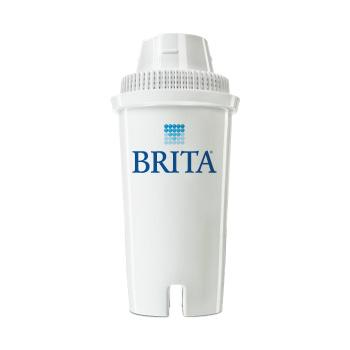
\includegraphics[height=0.5\textheight]{pics/brita}}

\begin{frame} 
  \titlepage
\end{frame}

\section{Fourier transform}
\begin{frame}
 \frametitle{Fourier series}
 \begin{block}{Definition of Fourier series of a function}
  If function $f(t)$ is \alert{periodic with period $T$}, then $a_n$ and $b_n$ exist such that
  \[ f(t) = \frac{a_0}{2} + \sum_{n=1,2,3,\ldots}^{+\infty} \left[ a_n \cos\left(\frac{2n\pi t}{T}\right) + b_n \sin\left(\frac{2n\pi t}{T}\right) \right] \]
  with
  \[ a_n = \frac{2}{T} \int_{-T/2}^{+T/2} f(t) \cos\left(\frac{2n\pi t}{T}\right) dt \]
  \[ b_n = \frac{2}{T} \int_{-T/2}^{+T/2} f(t) \sin\left(\frac{2n\pi t}{T}\right) dt \]
  The coefficients $a_n$ and $b_n$ indicate the strength of the harmonics with \alert{angular frequency $\omega_n = \frac{2n\pi}{T}$} or \alert{frequency $f_n = \frac{1}{T}$}.
 \end{block}
\end{frame}

\begin{frame}[t]
 \frametitle{Fourier series}
 \begin{block}{Example: Square wave}
  \begin{center}
   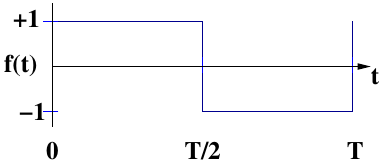
\includegraphics[width=0.5\textwidth]{pics/square_wave}
  \end{center}
  \[ f(t) = \frac{4}{\pi} \sum_{n=1,3,5,\ldots}^{+\infty} \frac{1}{n} \sin\left(\frac{2n\pi t}{T}\right) \]
 \end{block}
 \begin{block}{Live demo}
  \href{http://demonstrations.wolfram.com/FourierSeriesOfSimpleFunctions}{Fourier series of simple functions}
 \end{block}
\end{frame}

\begin{frame}[t]
 \frametitle{Fourier series}
 \begin{block}{Example: Square wave}
  \begin{center}
   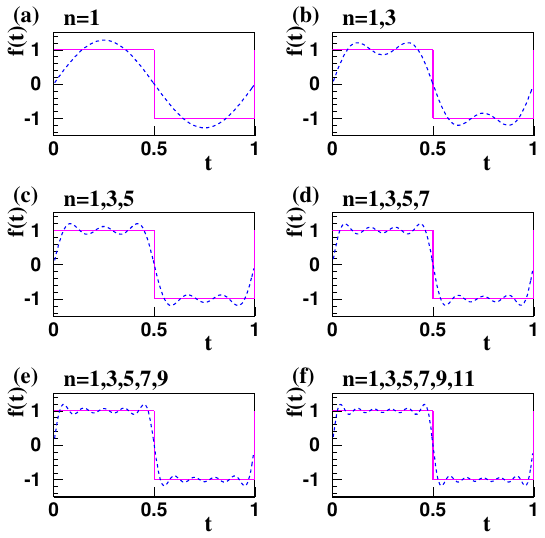
\includegraphics[width=0.48\textwidth]{pics/square_wave_approximation}
  \end{center}
  Filters (high-pass or low-pass) will have the effect of removing certain frequency harmonics.
 \end{block}
\end{frame}

\begin{frame}[t]
 \frametitle{Fourier series}
 \begin{block}{Power spectrum}
  Plot of coefficients $a_n$ and $b_n$ versus harmonic frequencies $\omega_n$
\only<1>{
 \[ f(t) = \frac{4}{\pi} \sum_{n=1,3,5,\ldots}^{+\infty} \frac{1}{n} \sin\left(\frac{2n\pi t}{T}\right) \quad \hbox{with}~b_n = \frac{4}{\pi}\frac{1}{n}, n=1,3,5,\ldots  \]
 }
 \end{block}
 \begin{block}<2>{Example: Square wave and triangle wave}
  \begin{center}
   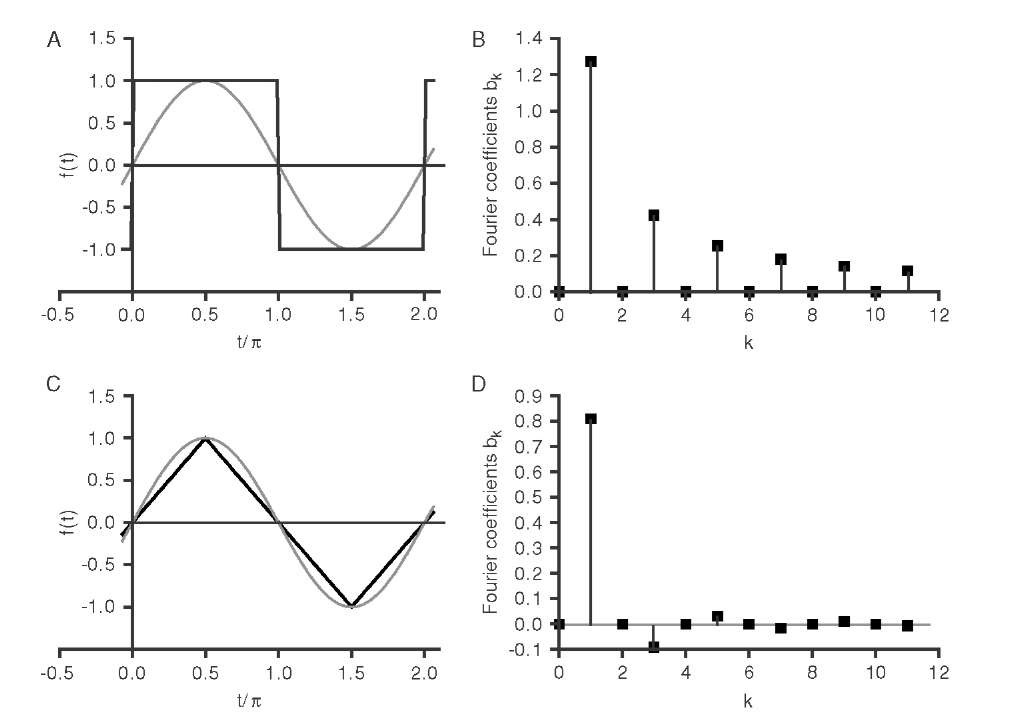
\includegraphics[width=0.65\textwidth]{pics/square_wave_b_n}
  \end{center}
 \end{block}
\end{frame}

\begin{frame}
 \frametitle{Fourier transform}
 \begin{block}{Definition of Fourier transform of a function}
  If function $f(t)$ goes to \alert{zero at $\pm \infty$}, then $F(\omega)$ exists such that
  \[ f(t) = \int^{+\infty}_{-\infty} F(\omega) e^{j \omega t} d\omega \]
  with
  \[ F(\omega) = \int^{+\infty}_{-\infty} f(t) e^{-j \omega t} dt \]
 \end{block}
 \begin{block}{Power spectrum}
  The Fourier transform $F(\omega)$ gives the strength \alert{for all frequencies}, not just the harmonics of some fundamental frequency.
 \end{block}
 \begin{block}{Live demo}
  \href{http://demonstrations.wolfram.com/ComparingFourierSeriesAndFourierTransform/}{Comparing Fourier series and Fourier transform}
 \end{block}
\end{frame}

\begin{frame}
 \frametitle{Fourier transform}
 \begin{block}{Example: Sine/cosine wave with $\omega_0$}
  Fourier transform is single ``$\delta$-spike'' at $\omega = \omega_0$, because no other frequency components are present.
  \[ f(t) = \cos\omega_0 t \Rightarrow F(\omega) = 0 \quad \hbox{for} \quad \omega \ne \omega_0 \]
 \end{block}
 \begin{block}{Example: Single square pulse (and basically every signal)}
  Because all frequency components are represented in the discontinuous step, the Fourier transform is non-zero for all value of $\omega$.
 \end{block}
 \begin{block}{Distortion due to systems}
  When a single pulse passes through a system that affects some frequency ranges differently, it will be distorted.
 \end{block}
\end{frame}

\begin{frame}
\frametitle{Fourier transform}
\begin{center}
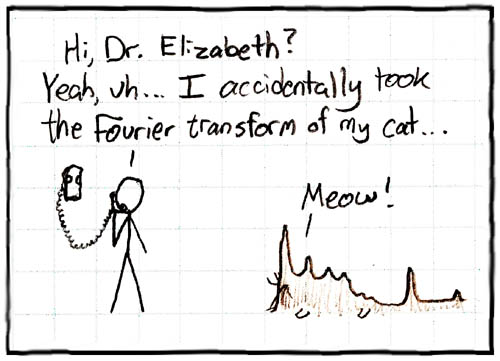
\includegraphics[height=0.7\textheight]{pics/fourier} \\
\href{http://xkcd.com/26}{xkcd/26}
\end{center}
\end{frame}


\section{Transfer function and Bode plots}
\begin{frame}
 \frametitle{Transfer function}
   \begin{columns}[t]
    \begin{column}{.45\textwidth}
     Time domain
     \begin{figure}
      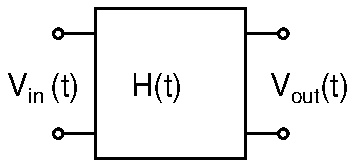
\includegraphics[width=0.55\textwidth]{./circuits/black_box_transfer_in_time.pdf}
     \end{figure}
     \[V_{out}(t)=\int^t_{-\infty} H(t-\tau) V_{in}(\tau) d \tau \]
    \end{column}
    \begin{column}{.45\textwidth}
     Frequency domain
     \begin{figure}
      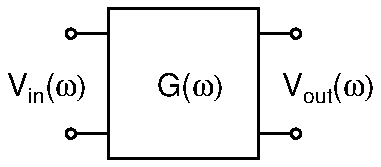
\includegraphics[width=0.55\textwidth]{./circuits/black_box_transfer_in_freq.pdf}
     \end{figure}
     \[V_{out}(\omega)=G(\omega) V_{in}(\omega) \]
     Where $G$ is complex transfer function or gain.
    \end{column}
   \end{columns}
   \begin{block}{Definition of gain}
    \[ G(\omega)=\frac{V_{out}(\omega)}{V_{in}(\omega)} = |G(\omega)| e^{j \phi(\omega)} \]
   \end{block}
   Often used values of $G$ in dB, with
   \[ dB = 20 \log_{10} (|G(w)|) \]
\end{frame}

\section{Filters}

 
\begin{frame}
 \frametitle{Simple example: RC low-pass filter}
     \begin{figure}
      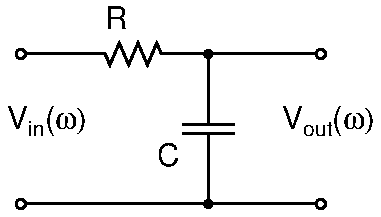
\includegraphics[width=0.25\textwidth]{./circuits/rc_low_pass.pdf}
     \end{figure}
    \[ G(\omega)
    =\frac{V_{out}(\omega)}{V_{in}(\omega)}
    = \frac{\frac{1}{j \omega C}}{R+\frac{1}{j \omega C}} 
    = \frac{1}{j \omega R C} \frac{1}{1+\frac{1}{j \omega R C}}
    = \frac{1}{1+j \omega R C}
    \]
    Define $\omega_{3dB}=\frac{1}{RC}$
    \[ G(\omega)
    = \frac{1}{1+j\frac{\omega}{\omega_{3dB}}}
    = \frac{1}{\sqrt{1+\frac{\omega^2}{\omega_{3dB}^2}}} e^{j \phi} ,
    \phi = atan (-\frac{\omega}{\omega_{3dB}})
    \]
    What does $\omega_{3dB}$ represent?
    \[
    |G(\omega=\omega_{3dB})|=20 \log_{10}\left(\frac{1}{\sqrt{1+1}}\right)
    =20 \log_{10}\left(\frac{1}{\sqrt{2}}\right)=-3 dB
    \]
\end{frame}


\begin{frame}
\frametitle{RC low-pass filter at $\omega=0.1/RC$}
\begin{columns}[c]
 \begin{column}{.55\textwidth}
  Signal vs time
  \begin{figure}
   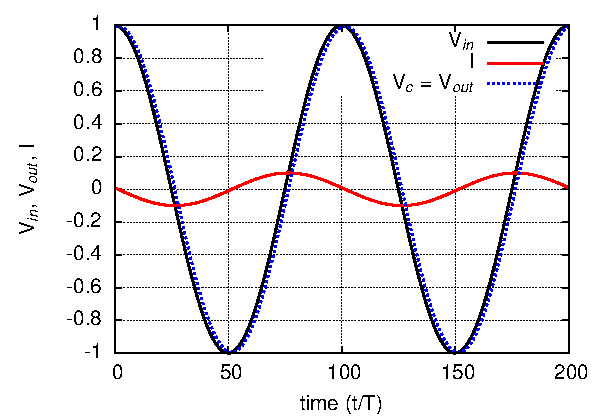
\includegraphics[angle=0,width=0.90\textwidth]{./plots/i_v_vr_w=_1rc}
  \end{figure}
 \end{column}
 \begin{column}{.45\textwidth}
  Lissajous plot
  \begin{figure}
   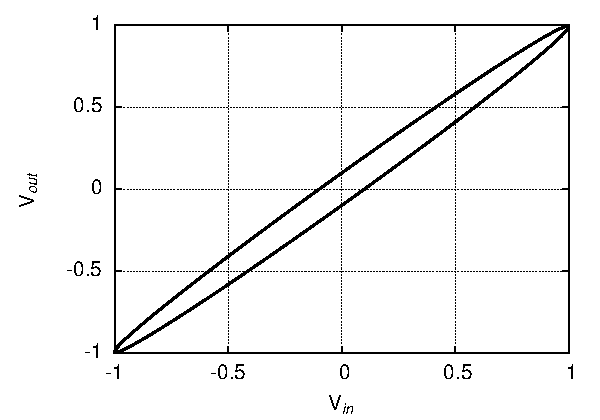
\includegraphics[angle=0,width=0.90\textwidth]{./plots/vc_vs_vin_w=_1rc}
  \end{figure}
 \end{column}
\end{columns}
\end{frame}

\begin{frame}
\frametitle{RC low-pass filter at $\omega=1/RC$}
\begin{columns}[c]
 \begin{column}{.55\textwidth}
  Signal vs time
  \begin{figure}
   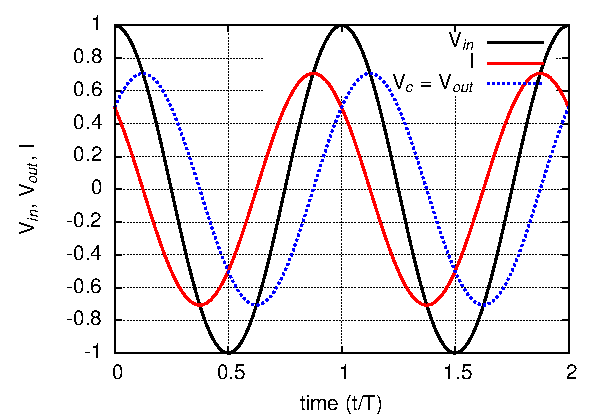
\includegraphics[angle=0,width=0.90\textwidth]{./plots/i_v_vr_w=rc}
  \end{figure}
 \end{column}
 \begin{column}{.45\textwidth}
  Lissajous plot
  \begin{figure}
   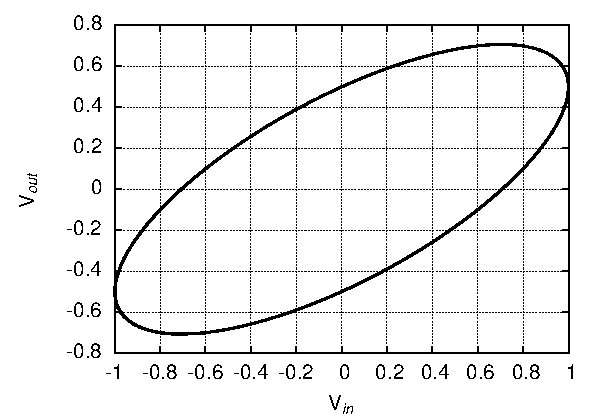
\includegraphics[angle=0,width=0.90\textwidth]{./plots/vc_vs_vin_w=rc}
  \end{figure}
 \end{column}
\end{columns}
\end{frame}

\begin{frame}
\frametitle{RC low-pass filter at $\omega=10/RC$}
\begin{columns}[c]
 \begin{column}{.55\textwidth}
  Signal vs time
  \begin{figure}
   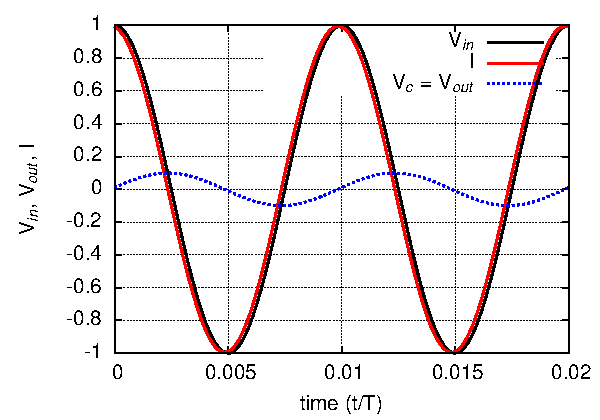
\includegraphics[angle=0,width=0.90\textwidth]{./plots/i_v_vr_w=10rc}
  \end{figure}
 \end{column}
 \begin{column}{.45\textwidth}
  Lissajous plot
  \begin{figure}
   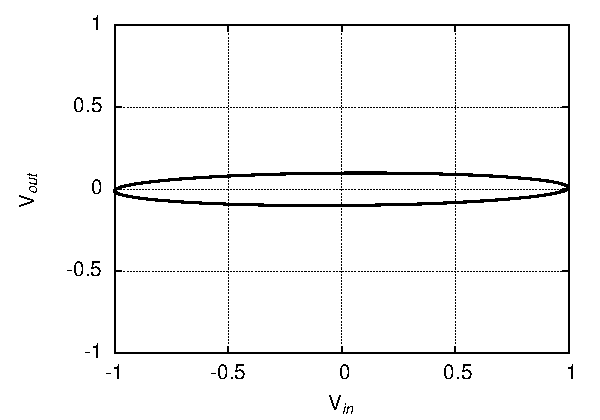
\includegraphics[angle=0,width=0.90\textwidth]{./plots/vc_vs_vin_w=10rc}
  \end{figure}
 \end{column}
\end{columns}
\end{frame}

\begin{frame}
\frametitle{Bode plots}
 \begin{block}{What are Bode plots?}
  Plots of magnitude and phase of the transfer function, where
  $|G|$ is often plotted in dB
 \end{block}
   \begin{columns}[c]
    \begin{column}{.25\textwidth}
     \begin{figure}
      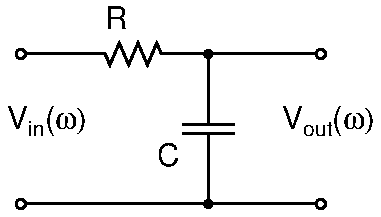
\includegraphics[width=1.00\textwidth]{./circuits/rc_low_pass.pdf}
     \end{figure}
    \[ G(\omega)
    = \frac{1}{1+j\frac{\omega}{\omega_{3dB}}}
    \]
    \end{column}
    \begin{column}{.75\textwidth}
      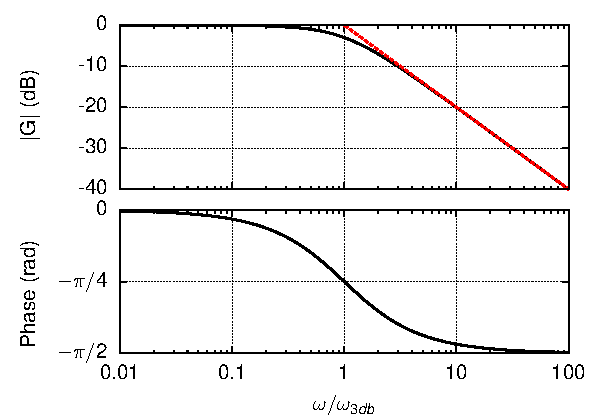
\includegraphics[angle=0,width=1.00\textwidth]{./plots/rc_low_pass_bode.pdf}
    \end{column}
   \end{columns}
\end{frame}

\begin{frame}
 \frametitle{Bode plots: Why in dB?}
 \begin{block}{Problem}
  You want to measure the 1\,$\mu$V fluctuations caused by the fast motion of atoms in an optical trap (at 6\,kHz).  The entire system is powered by 110\,V, 60\,Hz power from the grid, and you will need to filter this out.  What factor of 60\,Hz suppression noise do you need (in dB)?
 \end{block}
 \begin{block}<2>{Discussion}
  \begin{itemize}
   \item Let's assume that you want a 10-to-1 signal-to-noise ratio, then the maximum voltage at 60\,Hz is 100\,nV.  You need a suppression by a factor $10^9$, or 180\,dB.
   \item You look in your lab and find some RC filters with a factor 177.8 suppression.  How many would you need?
   \item You look a bit further and find some RC filters with 45\,dB suppression.  How many of these would you need?
   \item Will it work?  (We'll come back to this\ldots)
  \end{itemize}
 \end{block}
\end{frame}
 
\begin{frame}[t]
 \frametitle{Bode plots: Filter theory (a little bit)}
 \begin{block}{Characteristics of a Bode plot}
  \begin{itemize}
   \item Straight lines in log-log plots (major advantage of dB scale)
   \item 3dB frequencies are cut-off points: $\omega_{3dB}$ where $|G(\omega)| = 3\,dB$
   \item Power roll-off: goes like $\omega^n$ ($n$ is the order of the filter)
   \begin{itemize}
    \item For first-order filters, $n = 1$, and one decade in $\omega$ corresponds to a 20\,dB reduction
   \end{itemize}
  \end{itemize}
 \end{block}
 \begin{block}{Filter theory in a nut shell}
  The gain $G(\omega)$ can be written as $G(\omega) = A \prod_n \frac{(\omega + j z_n)^{a_n}}{(\omega + j p_n)^{b_n}}$ with zeroes $z_n$ and poles $p_n$ (with multiplicities $a_n$ and $b_n$).
  \begin{itemize}
   \item Start with constant magnitude for $\omega = 0$
   \item Each pole or zero will result in a 20\,dB/decade change of slope per multiplicity (down for poles, up for zeroes).
   \item At each pole or zero you adjust the plot by 3\,dB.
  \end{itemize}
 \end{block}
\end{frame}


\begin{frame}
\frametitle{RC high-pass filter}
   \begin{columns}[c]
    \begin{column}{.25\textwidth}
     \begin{figure}
      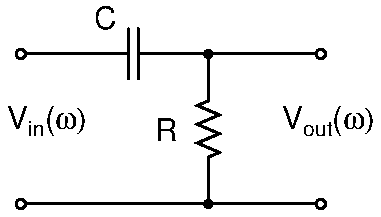
\includegraphics[width=1.00\textwidth]{./circuits/rc_high_pass.pdf}
     \end{figure}
    \end{column}
    \begin{column}{.75\textwidth}
      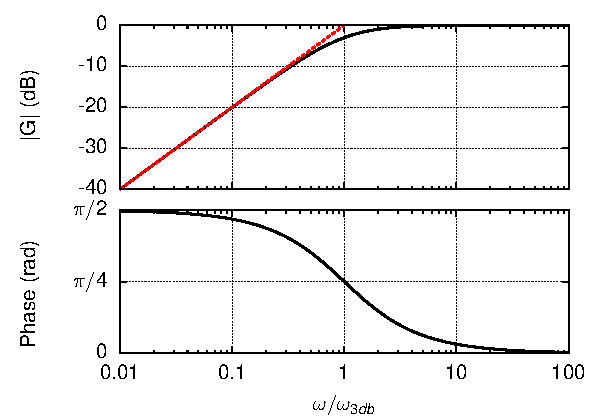
\includegraphics[angle=0,width=1.00\textwidth]{./plots/rc_high_pass_bode.pdf}
    \end{column}
   \end{columns}
    \[ G(\omega)
    =\frac{V_{out}(\omega)}{V_{in}(\omega)}
    = \frac{R}{R+\frac{1}{j \omega C}} 
    = \frac{j \omega R C}{1+j \omega R C}
    = \frac{j \frac{\omega}{\omega_{3dB}}}{1+j\frac{\omega}{\omega_{3dB}}}
    \]
    with $\omega_{3dB}=\frac{1}{RC}$
\end{frame}

\begin{frame}
 \frametitle{Bode plots: Filter theory (a little bit)}
 \begin{block}{Drawing the RC high-pass filter Bode diagram}
  \begin{itemize}
   \item Zero at $\omega = 0$ (multiplicity of 1).
   \item Line from $\omega = 0$ to $\omega = \omega_{3dB}$ increases by 20\,dB/decade.
   \item Pole at $\omega = \omega_{3dB}$ (multiplicity of 1).
   \item Slope changes by 20\,dB/decade, then remains constant for $\omega \to \infty$.
  \end{itemize}
 \end{block}
\end{frame}


\begin{frame}
\frametitle{RL filters}
   \begin{columns}[c]
    \begin{column}{.50\textwidth}
     RL low-pass filter
     \begin{figure}
      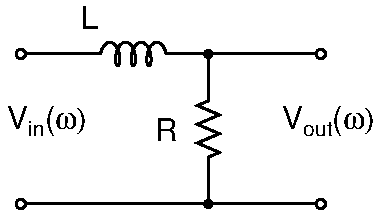
\includegraphics[width=0.50\textwidth]{./circuits/rl_low_pass.pdf}
     \end{figure}
     \[
     G(\omega) 
     = \frac{R}{R+j\omega L},
     \omega_{3dB}=\frac{R}{L}
     \]
     \vskip -.3in
     \begin{figure}
      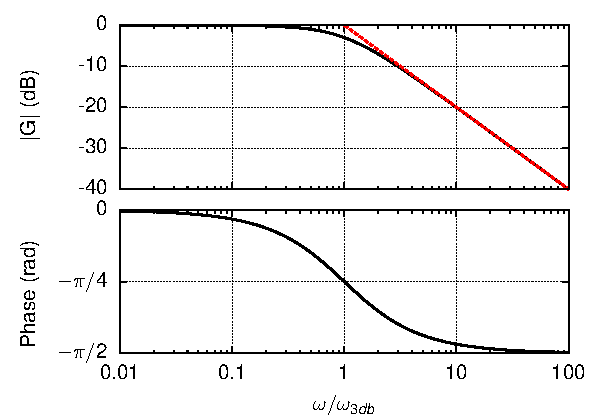
\includegraphics[angle=0,width=1.0\textwidth]{./plots/rl_low_pass_bode.pdf}
     \end{figure}
    \end{column}
    \begin{column}{.50\textwidth}
     RL high-pass filter
     \begin{figure}
      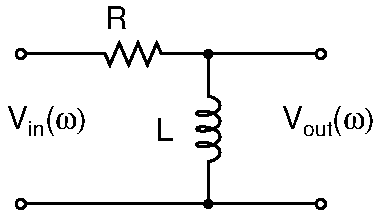
\includegraphics[width=0.5\textwidth]{./circuits/rl_high_pass.pdf}
     \end{figure}
     \[
     G(\omega)
     = \frac{j \omega L}{R+j\omega L}
     \]
     \vskip -.3in
     \begin{figure}
      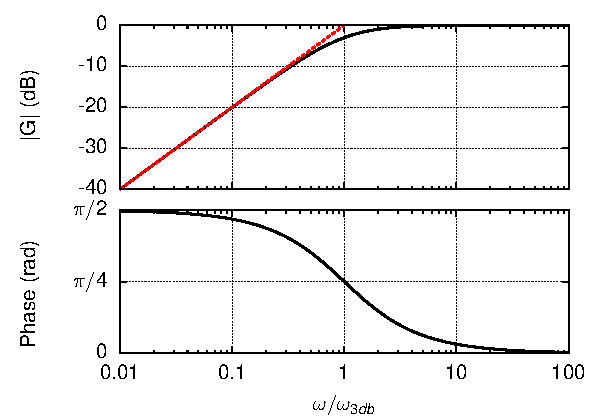
\includegraphics[angle=0,width=1.0\textwidth]{./plots/rl_high_pass_bode.pdf}
     \end{figure}
    \end{column}
   \end{columns}
\end{frame}

\subsection{Loaded vs unloaded filter}
\begin{frame}
 \frametitle{Voltage divider}
 \begin{columns}[c]
  \begin{column}{.4\textwidth}
   \includegraphics<1>[height=2in]{./pics/unloaded_voltage_divider}
   \includegraphics<2>[height=2in]{./pics/loaded_voltage_divider}
  \end{column}
  \begin{column}{.6\textwidth}
   \begin{itemize}
    \item Gain $G = \frac{V_{out}}{V_{in}} = \frac{R_2}{R_1 + R_2}$
    \item What is the resistance $V_{in}$ sees?
    \[ R_{in} = R_1 + R_2 \]
    \item What is the Th\'{e}venin resistance?
    \[ R_{out} = R_{1 \parallel 2} \]
    \item<2> Rule of 10: if $R_L > 10 R_{out}$, then the voltage $V_{out}$ will be virtually unchanged
   \end{itemize}
  \end{column}
 \end{columns}
\end{frame}

\begin{frame}
 \frametitle{Input and output impedances}
 \begin{center}
  \begin{circuitikz}
   \draw (-2,2) node[left]{$v_{in}$} to[R,l=$R$,o-] (0,2) to[C,l=$C$] (0,0.5) node[ground]{};
   \draw (0,2) to[short,-o] (1,2) node[right]{$v_{out}$};
  \end{circuitikz}
 \end{center}
 \begin{columns}[t]
  \begin{column}{0.48\textwidth}
   \begin{block}{Input impedance $Z_{in}$}
    \begin{itemize}
     \item What is the impedance a driving circuit sees?
     \item Assume large load $Z_L$ is connected (rule of 10).
     \item<2-> R and C in series: $Z_{in} = R + \frac{1}{j\omega C}$
    \end{itemize}
   \end{block}
  \end{column}
  \begin{column}{0.48\textwidth}
   \begin{block}{Output impedance $Z_{out}$}
    \begin{itemize}
     \item What is the Th\'evenin impedance of the filter?
     \item Assume small internal resistance of driving circuit.
     \item<3-> R and C in parallel: $Z_{out} = \frac{V_{Th}}{I_{N}} = \frac{R}{1 + j\omega RC}$
    \end{itemize}
   \end{block}
  \end{column}
 \end{columns}
\end{frame}

\begin{frame}
 \frametitle{Filters chain}
 \begin{figure}
  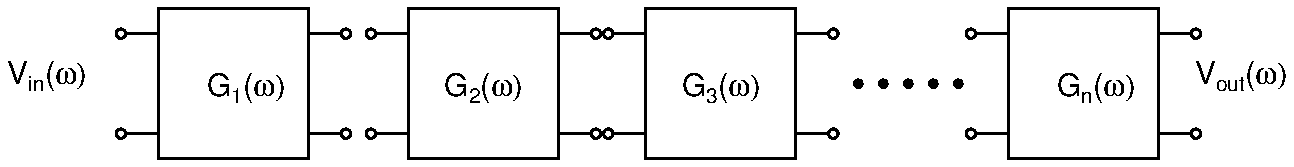
\includegraphics[angle=0,width=1.0\textwidth]{./circuits/black_box_transfer_in_freq_chain.pdf}
 \end{figure}
 Technically next stage loads the previous and it is quite hard to
 calculate total transfer function.

 However we use rule of 10 to avoid overloading the previous filter.\\
 Every next stage resistor $|Z_{in,i+1}| > 10 |Z_{out,i}|$ we can approximate
 \[
 G_t(\omega) \approx G_1(\omega) G_2(\omega) G_3(\omega) \cdots G_n(\omega)
 \]
\end{frame}

\frame
{ \frametitle{ Example band pass filter}
\begin{figure}
 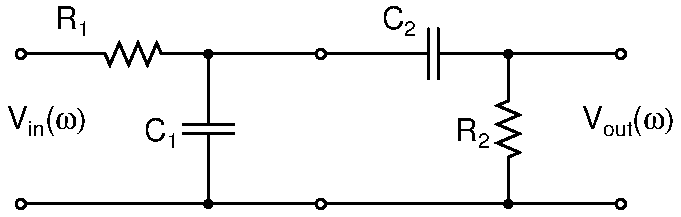
\includegraphics[angle=0,width=0.5\textwidth]{./circuits/band_pass_filter.pdf}
\end{figure}
\begin{columns}
 \begin{column}{.50\textwidth}
  \[
  G_t(\omega) \approx G_1(\omega) G_2(\omega) 
  \]
  \[
  G_t(\omega) \approx
  \frac{1}{1+j\frac{\omega}{\omega_{1_{3dB}}}}
  \frac{j \frac{\omega}{\omega_{2_{3dB}}}}{1+j\frac{\omega}{\omega_{2_{3dB}}}}
  \]
  For $R_1=1 k\Omega, R_2=100 k\Omega$,\\
  $C_1=C_2=.01 \mu F$
 \end{column}
 \begin{column}{.50\textwidth}
  \vskip -.2in
  \begin{figure}
   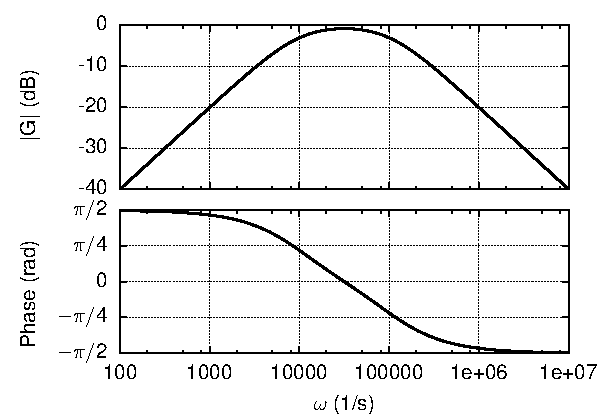
\includegraphics[angle=0,width=1.0\textwidth]{./plots/rc_band_pass_bode.pdf}
  \end{figure}
 \end{column}
\end{columns}
}

\frame
{ \frametitle{Notch filter - Band stop filter}
\vskip -0.4in
\begin{columns}
 \begin{column}{.250\textwidth}
  \begin{figure}
   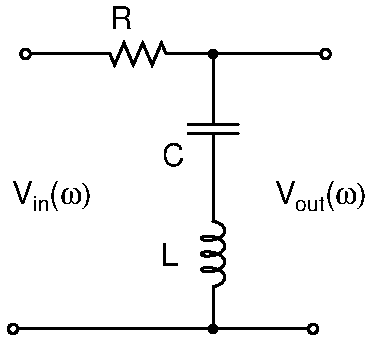
\includegraphics[angle=0,width=1.00\textwidth]{./circuits/rlcnotch.pdf}
  \end{figure}
  \[
  \omega_0=\frac{1}{\sqrt{LC}}
  \]
 \end{column}
 \begin{column}{.750\textwidth}
  \begin{figure}
   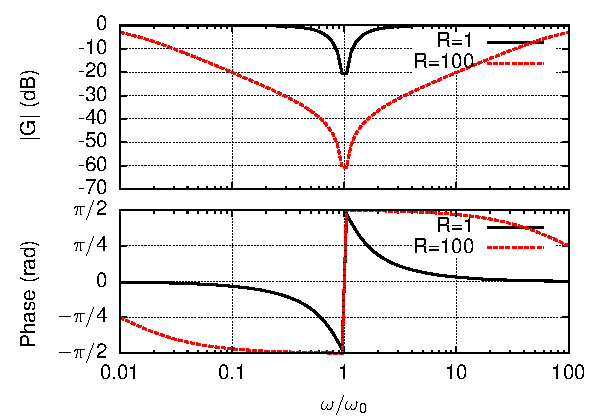
\includegraphics[angle=0,width=1.0\textwidth]{./plots/rlc_notch_bode.pdf}
  \end{figure}
 \end{column}
\end{columns}
\alert{It is impossible to make band stop filter with $G\approx1$ outside
of stop band with only simple combinations of low and high-pass filters.}
R, L, and C combo is required or a complicated network of R-C, R-L elements.
}

\subsection{RLC filters}
\begin{frame}
 \frametitle{RLC filters}
 \begin{columns}
  \begin{column}{0.4\textwidth}
   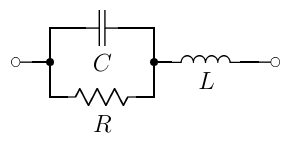
\includegraphics[width=\textwidth]{pics/RLC_circuit}
  \end{column}
  \begin{column}{0.6\textwidth}
   \begin{itemize}
    \item $\omega_{LC} = \frac{1}{\sqrt{LC}}$
    \item $\omega_{RC} = \frac{1}{RC}$
    \item $\omega_{RL} = \frac{R}{L}$
   \end{itemize}
   Note: $\omega_{RC} \omega_{RL} = \omega^2_{LC}$
  \end{column}
 \end{columns}
 \begin{block}{Three output voltages}
  \begin{columns}
   \begin{column}{0.5\textwidth}
    \begin{itemize}
     \item $v_o^R(\omega)$ across resistor
     \item $v_o^L(\omega)$ across inductor
     \item $v_o^C(\omega)$ across capacitor
    \end{itemize}
   \end{column}
   \begin{column}{0.5\textwidth}
    Typically $R$ and $L$ in one component, so measure $v_o^R(\omega) + v_o^L(\omega)$
   \end{column}
  \end{columns}
 \end{block}
\end{frame}

\begin{frame}
 \frametitle{RLC filters}
 \begin{block}{Total impedance}
  \begin{equation*}
   Z_{tot} = R + j\omega L + \frac{1}{j\omega C} = R \left[ 1 - j\frac{\omega_{RC}}{\omega} \left( 1 - \frac{\omega^2}{\omega_{LC}^2} \right) \right]
  \end{equation*}
 \end{block}
 \begin{block}{Voltage divider: gain across capacitor}
  \begin{equation*}
   G_C(\omega) = \frac{Z_C}{Z_{tot}} = \frac{1}{j\omega RC\left[ 1 - j\frac{\omega_{RC}}{\omega} \left( 1 - \frac{\omega^2}{\omega_{LC}^2} \right) \right]} = \frac{1}{\left( 1 - \frac{\omega^2}{\omega_{LC}^2} \right) + j\frac{\omega}{\omega_{RC}}}
  \end{equation*}
  \begin{eqnarray*}
   |G_C(\omega)| & = & \frac{1}{\sqrt{ \left(1 - \omega^2/\omega_{LC}^2 \right)^2 + \omega^2/\omega^2_{RC}}} \\
   \phi_C & = & \tan^{-1} \frac{- \omega/\omega_{RC}}{1 - \omega^2/\omega_{LC}^2}
  \end{eqnarray*}
 \end{block}
\end{frame}

\begin{frame}
 \frametitle{RLC filters: gain across capacitor}
 \begin{block}{Resonance at $\omega = \omega_{LC}$}
  \begin{itemize}
   \item $|G_C(\omega)| = \frac{\omega_{RC}}{\omega_{RL}} = \sqrt{\frac{L}{R^2 C}}$ large for $R$ small
   \item $\phi_C = -\frac{\pi}{2}$
  \end{itemize}
 \end{block}
 \begin{block}{Low frequency limit}
  \begin{itemize}
   \item $|G_C(\omega)| \to 1$
   \item $\phi_C \to 0$
  \end{itemize}
 \end{block}
 \begin{block}{High frequency limit}
  \begin{itemize}
   \item $|G_C(\omega)| \to \frac{\omega^2_{LC}}{\omega^2}$
   \item $\phi_C \to -\pi$
  \end{itemize}
 \end{block}
\end{frame}

\begin{frame}
 \frametitle{RLC filters: gain across capacitor}
 \begin{center}
  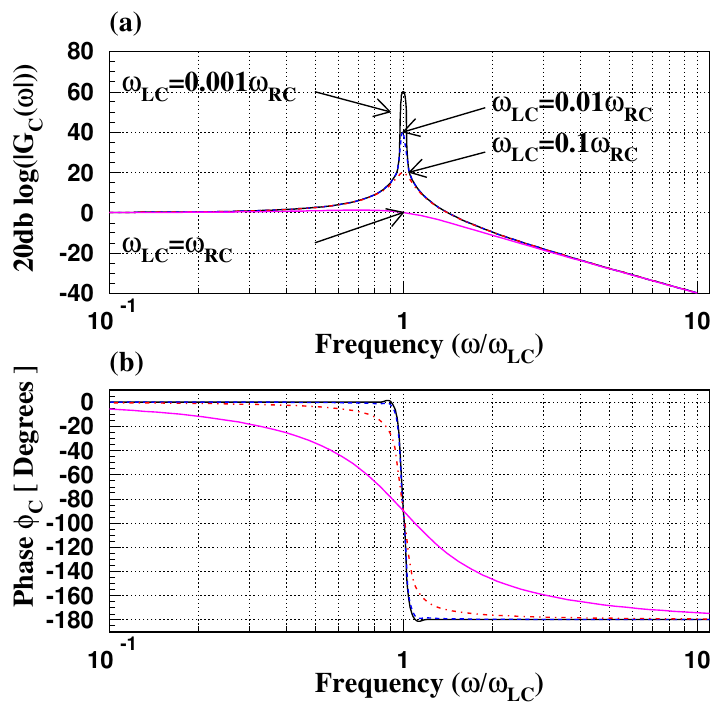
\includegraphics[width=0.6\textwidth]{pics/RLC_bode_capacitor}
 \end{center}
\end{frame}

\begin{frame}
 \frametitle{RLC filters}
 \begin{block}{Voltage divider: gain across inductor}
  \begin{equation*}
   G_L(\omega) = \frac{Z_L}{Z_{tot}} = \frac{j\omega L}{R\left[ 1 - j\frac{\omega_{RC}}{\omega} \left( 1 - \frac{\omega^2}{\omega_{LC}^2} \right) \right]} = \frac{1}{\left( 1 - \frac{\omega^2_{LC}}{\omega^2} \right) + j\frac{\omega_{RL}}{\omega}}
  \end{equation*}
  \begin{eqnarray*}
   |G_L(\omega)| & = & \frac{1}{\sqrt{ \left(1 - \omega_{LC}^2/\omega^2 \right)^2 + \omega_{RL}^2/\omega^2}} \\
   \phi_L & = & \tan^{-1} \frac{\omega_{RL}/\omega}{1 - \omega_{LC}^2/\omega^2}
  \end{eqnarray*}
 \end{block}
\end{frame}

\begin{frame}
 \frametitle{RLC filters: gain across inductor}
 \begin{block}{Resonance at $\omega = \omega_{LC}$}
  \begin{itemize}
   \item $|G_L(\omega)| = \frac{\omega_{LC}}{\omega_{RL}} = \sqrt{\frac{L}{R^2 C}}$ large for $R$ small
   \item $\phi_L = \frac{\pi}{2}$
  \end{itemize}
 \end{block}
 \begin{block}{Low frequency limit}
  \begin{itemize}
   \item $|G_L(\omega)| \to \frac{\omega^2}{\omega_{LC}^2}$
   \item $\phi_L \to \pi$
  \end{itemize}
 \end{block}
 \begin{block}{High frequency limit}
  \begin{itemize}
   \item $|G_L(\omega)| \to 1$
   \item $\phi_L \to 0$
  \end{itemize}
 \end{block}
\end{frame}

\begin{frame}
 \frametitle{RLC filters: gain across inductor}
 \begin{center}
  \includegraphics[width=0.6\textwidth]{pics/RLC_bode_inductor}
 \end{center}
\end{frame}

\begin{frame}
 \frametitle{RLC filters: gain larger than 0\,dB}
 \begin{columns}
  \begin{column}{0.5\textwidth}
   \includegraphics[width=\textwidth]{pics/RLC_bode_capacitor}   
  \end{column}
  \begin{column}{0.5\textwidth}
   \includegraphics[width=\textwidth]{pics/RLC_bode_inductor}
  \end{column}
 \end{columns}
 \begin{block}{Gain larger than 1}
  Possible when the phase is opposite:
  \begin{itemize}
   \item $v_C(t) + v_L(t) = 0$
  \end{itemize}
 \end{block}
\end{frame}


\end{document}


\end{document}

\documentclass{article}


% This file is a solution template for:
% 1 inch margins
\usepackage{fullpage}

\usepackage{booktabs}
\usepackage{longtable}

\usepackage{hyperref}
\usepackage{graphicx}
\usepackage{multicol}
\usepackage{subcaption}

% Add ability to resume enumeration environments with /begin{enumerate}[resume]
\usepackage{enumitem}

\usepackage{pgf}
\usepackage{tikz}
\usepackage{bodegraph}
\usepackage{circuitikz}
\usetikzlibrary{calc}
\usetikzlibrary{trees}
\usetikzlibrary{arrows}
\usetikzlibrary{shapes}
\usetikzlibrary{fadings}
\usetikzlibrary{positioning}
\usetikzlibrary{intersections}


\usepackage[english]{babel}
\usepackage[latin1]{inputenc}
\usepackage[T1]{fontenc}
% Or whatever. Note that the encoding and the font should match. If T1 does not look nice, try deleting the line with the fontenc.


\usepackage{listings}

\usepackage{amsmath}


\usepackage{xspace}
\newcommand{\Ohm}{$\Omega$\xspace}



\title{Capacitors, Inductors, and Complex Impedance}


\begin{document}
\maketitle

In this chapter we introduce the concept of complex resistance, or \emph{impedance}, by studying two reactive circuit elements, the \emph{capacitor} and the \emph{inductor}. We will study capacitors and inductors using differential equations and Fourier analysis and from these derive their impedance. Capacitors and inductors are used primarily in circuits involving time-dependent voltages and currents, such as AC circuits.

\section{AC Voltages and circuits}
Most electronic circuits involve time-dependent voltages and currents. An important class of time-dependent signal is the sinusoidal voltage (or current), also known as an AC signal (Alternating Current). \emph{Kirchhoff's laws and Ohm's law still apply (they always apply), but one must be careful to differentiate between time-averaged and instantaneous quantities.}

An AC voltage (or signal) is of the form:
\begin{equation}
v(t) = V_0 \cos\omega t
\end{equation}
where $\omega$ is the angular frequency, $V_0$ is the amplitude of the waveform or the \emph{peak voltage} and $t$ is the time. The angular frequency is related to the frequency $f$ by $\omega = 2 \pi f$, and the period $T$ is related to the frequency by $T = \frac{1}{f}$. Other useful voltages are also commonly defined. They include the \emph{peak-to-peak voltage} ($V_{pp}$) which is twice the amplitude $V_0$, and the RMS voltage ($V_{RMS}$) which is $V_{RMS} = V_0 / \sqrt{2}$. The average power dissipated in a resistive AC device is computed using RMS quantities:
\begin{equation}
P = I_{RMS} V_{RMS} = \frac{1}{2} I_0 V_0.
\end{equation}
This is important enough that voltmeters and ammeters in AC mode actually return the RMS values for current and voltage.

While most real world signals are not sinusoidal, AC signals are still used extensively to characterize circuits through the technique of Fourier analysis.

\subsection{Fourier Analysis}
One convenient way to characterize the rate of change of a function is to write the true function as a linear combination of a set of functions that have particularly easy characteristics to deal with analytically. In this case we can consider the trigonometric functions. It turns out that we can write any function as an integral of the form
\begin{equation}
v(t) = \int v(\omega) \cos \left( \omega t + \phi(\omega) \right) d\omega
\end{equation}
where $v(\omega)$ and $\phi(\omega)$ are functions of the frequency $\omega$. This process is called Fourier analysis, and it means that any function can be written as an integral of simple sinusoidal functions. In the case of a periodic waveform this integral becomes a sum over all the harmonics of the period (i.e. all the integer multiplicative frequencies of the period).
\begin{equation}
v(t) = \sum_n A_n \cos (n\omega t + \phi_n).
\end{equation}
An implication of this mathematical fact is that \emph{if we can figure out what happens when we put pure sinusoidal voltages into a linear circuit, then we will know everything about its operation even for arbitrary input voltages.}

\subsection{Complex Notation}
In complex notation we replace our sinusoidal functions by exponentials to make the calculus and bookkeeping easier still. Then we can include both phase and magnitude
information. We'll define 
\begin{equation}
e^{j\phi} = \cos\phi + j\sin\phi,
\end{equation}
where $j^2 = -1$.

The general procedure for using this notation is:
\begin{enumerate}
\item Change your problem into complex algebra, i.e. replace $\cos\omega t$ with $e^{j \omega t}$.
\item Solve the problem.
\item Take the real part of the solution as your answer at the end.
\end{enumerate}


\section{Capacitors}
One of the most basic rules of electronics is that circuits must be complete for currents to flow. This week, we will introduce an exception to that rule.

The capacitor is actually a small break in a circuit. Try measuring the resistance of a capacitor, you will find that it is an open circuit. However, at the inside ends of the capacitor's lead, it has little plates that act as charge reservoirs where it can store charge. For short times, you do not notice that the break is there. Negative charge initially flows in to one side and out from out the other side just as if the two leads were connected. For fast signals, the capacitor ``looks'' like a short-circuit. But after a while the capacitor's reservoirs fill, the current stops, and we notice that there really is a break in the circuit.

For slow signals, a capacitor ``looks'' like an open circuit. What is fast, and what is slow? It depends on the capacitor and the rest of the circuit. This week, you will learn how to determine fast and slow for yourselves.

Capacitors serve three major roles in electrical circuits (although all three are just variations of one basic idea):
\begin{itemize}
\item Charge integrators;
\item High or low frequency filters;
\item DC isolators.
\end{itemize}

In order to perform these functions analytically, we will need to introduce a number of new concepts and some significant mathematical formalism. In this process we will also develop a number of new concepts in analyzing electronic circuits.

\subsection{Capacitance}
A capacitor is a device for storing charge and electrical energy. It consists of two parallel conducting plates and some non-conducting material between the plates, as shown in Figure~\ref{fig:capacitor}. When voltage is applied positive charge collects on one plate and negative charge collects on the other plane. Since they are attracted to each other this is a stable state until the voltage is changed again.

A capacitor's charge capacity or capacitance ($C$) is defined as:
\begin{equation}
 Q = C V
\end{equation}
which relates the charge stored in the capacitor ($Q$) to the voltage across its leads ($V$). Capacitance is measured in Farads (F). A Farad is a very large unit and most applications use $\mu$F, nF, or pF sized devices. Many electronics components have small parasitic capacitances due to their leads and design.

The capacitor also stores energy in the electric field generated by the charges on its two plates. The potential energy stored in a capacitor with voltage $V$ on it is
\begin{equation}
 E = \frac{1}{2} C V^2
\end{equation}
We usually speak in terms of current when we analyze a circuit. By noting that the current is the rate of change of charge, we can rewrite the definition of capacitance in terms of the current as:
\begin{eqnarray}
v & = & \frac{q}{C} = \frac{1}{C} \int i dt \\
i & = & C \frac{dv}{dt} = C \dot{v}
\end{eqnarray}
This shows that we can integrate a function $i(t)$ just by monitoring the voltage as the current charges up a capacitor, or we can differentiate a function $v(t)$ by putting it across a capacitor, and monitoring the current flow when the voltage changes.

\begin{figure}
\begin{center}
\includegraphics[width=0.4\textwidth]{pics/capacitor}
\end{center}
\caption{ A capacitor consist of two parallel plates which store equal and opposite amounts of charge.}
\label{fig:capacitor}
\end{figure}

\subsection{A Simple RC Circuit}

We will start by looking in detail at the simplest capacitive circuit, which is shown in Figure~\ref{fig:RC_circuit}. An RC circuit is made by simply putting a resistor and a capacitor together as a voltage divider. We will put the resistor in first, so we can connect the capacitor to ground.

By applying Kirchhoff's Laws to this circuit, we can see that:
\begin{itemize}
\item The same current flows through both the resistor and the capacitor, and
\item The sum of the voltage drops across the two elements equal the input voltage.
\end{itemize}
This can be put into a formula in the following equation:
\begin{equation}
v_{in} = i R + \frac{1}{C} \int i dt
\end{equation}
which can also be written as
\begin{equation}
\frac{v_{in}}{R} = i + \frac{1}{RC} \int i dt
\end{equation}
We can also put this into the form of a differential equation in the following way:
\begin{eqnarray}
\frac{dv_{in}}{dt} & = & R \frac{di}{dt} + \frac{i}{C}  \nonumber \\
C \dot{v}_{in} & = & R C \dot{i} + i
\label{eqn:RC_diffeqn}
\end{eqnarray}
These equations show that times are measured in units of $RC$, and that what you see depends on how quickly things change during one $RC$ time interval.

If the current changes quickly, then most of the voltage will show up across the resistor, while the voltage across the capacitor slowly charges up as it integrates the current. If the voltage changes slowly, then most of the voltage shows up across the capacitor as it charges. Since this usually requires a small current, the voltage across the resistor stays small.

But, what happens at intermediate times? To determine this quantitatively we will have to develop some more sophisticated mathematical techniques.

\subsection{Solutions to $RC$ Circuit}
Rather than produce the general solution, we will concentrate on two special cases that are particularly useful. The first will be for a constant voltage and the second will be a sinusoidal input.

\begin{figure}
 \begin{center}
  \begin{circuitikz}
   \draw (-2,0) node[ground]{} to[battery1,l=$v_{in}$] (-2,2) to[R,l=$R$] (0,2) to[C,l=$C$] (0,0) node[ground]{};
   \draw (0,2) to[short,-o] (1,2) node[right]{$v_{out}$};
  \end{circuitikz}
 \end{center}
 \caption{A simple RC circuit which integrates current.}
 \label{fig:RC_circuit}
\end{figure}

To study a constant supply voltage on an RC circuit, we set the left side of equation~\ref{eqn:RC_diffeqn} equal to a constant voltage. Then we have a simple homogeneous differential equation with the simple solution for the current of a decaying exponential,
\begin{equation}
 i = I_0 e^{-t/RC}
\end{equation}
which will account for any initial conditions. After a time of a few RC time periods, this solution will have decayed away to the supply voltage.

And now let us consider the other solution. In the prior section, we argued that if we can understand the $RC$ circuit's behavior for sinusoidal input we can deal with any arbitrary input. Therefore, this is the important one.

Let's look at our simple $RC$ circuit and suppose that we apply (or drive) a simple sine wave into the input:
\begin{equation}
v_{in} = V_0 \cos \omega t
\label{eqn:RC_voltage_cos}
\end{equation}
In complex notation, this means that we will set the drive voltage to
\begin{equation}
v_{in} = \Re \left(V_0 e^{j \omega t}\right)
\label{eqn:RC_voltage_exp}
\end{equation}
and we just have to remember to take the real part at the end of our calculation.

If we put this drive voltage into the differential equation \ref{eqn:RC_diffeqn}, then it becomes a relatively simple inhomogeneous differential equation:
\begin{equation}
C \frac{dv_{in}}{dt} = j \omega C V_0 e^{j \omega t} = R C \frac{di}{dt} + i.
\end{equation}
This is relatively simple because it shows up so often in physics that you might as well memorize the solution or at least the way to get the solution. Note that mathematically it looks just like a driven harmonic oscillator.

We can obtain the solution by using the standard recipe for first order linear differential equations. We start by rewriting equation as
\begin{equation}
\frac{di}{dt} + \frac{1}{R C} I = j \omega \frac{1}{R} V_0 e^{j \omega t}
\end{equation}
which we then multiply by $e^{t/RC}$ to obtain
\begin{equation}
e^{t/RC} \frac{di}{dt} + e^{t/RC} \frac{1}{R C} i = j \omega \frac{1}{R} V_0 e^{j \omega + \frac{1}{RC} t}.
\end{equation}

The left hand-side of this equality can be rewritten under the form of a total derivative (multiplication rule) so that we now have
\begin{equation}
\frac{d}{dt}\left[ i(t) e^{\left(t/RC\right)}\right] = \frac{j\omega V_0}{R} e^{\left( j\omega t + t/RC \right)}.
\end{equation}
This equation is easily integrable and can be rewritten as
\begin{equation}
i(t) e^{\left(t/RC\right)} = \frac{j\omega V_0}{R} \int e^{\left(j\omega t + t/RC\right)} dt.
\end{equation}
The integral is straightforward and yields the following expression:
\begin{equation}
i(t) = \frac{j\omega V_0}{R} \frac{1}{\frac{1}{RC} + j\omega} e^{\left(j\omega t\right)} + \hbox{constant} \cdot e^{\left( -t/RC \right)}.
\end{equation}
The first term represents the ``steady state'' oscillatory behavior of the driven circuit, while the second term describes the transient behavior of the current after switching on the driving voltage. Since we are only interested in the long-term behavior of the circuit, we neglect the second term and concentrate on the first. After a little bit of algebra, we can rewrite the steady-state current as
\begin{equation}
i(t) = \frac{j\omega V_0}{R} \frac{1}{\frac{1}{RC} + j\omega} e^{\left(j\omega t\right)} = \frac{\omega V_0 C}{\sqrt{1 + (\omega RC)^2}} \frac{\omega RC + j}{\sqrt{1 + (\omega RC)^2}} e^{\left(j\omega t\right)}.
\end{equation}
The second fraction can be interpreted as a phase term with $\tan\phi = \frac{1}{\omega RC}$, so that the expression for the current becomes
\begin{equation}
i(t) = I_0 e^{\left(j\omega t + \phi\right)}
\label{eqn:current_in_RC_circuit}
\end{equation}
with
\begin{equation}
I_0 = \frac{\omega V_0 C}{\sqrt{1 + \left(\omega RC\right)^2}} = \frac{V_0}{R} \cos\phi.
\end{equation}
The real solution of this simple RC circuit can be obtained by taking the real part of equation~\ref{eqn:current_in_RC_circuit}, and is left as an exercise to the reader.

The solution of the simple RC circuit appears to be rather complicated and involved, however it simplifies considerably when we plug equation~\ref{eqn:current_in_RC_circuit} back in to the original integral equation from Kirchhoff's loop law (equation~\ref{eqn:RC_diffeqn}). After integrating the exponential and a little bit of algebra, we obtain
\begin{equation}
v_{in}(t;\omega) = i(t) R + i(t) \frac{1}{j\omega C}
\end{equation}
This remarkably simple expression looks a lot like the standard Kirchhoff's loop law for resistors, except that the capacitor term behaves with a frequency dependent ``imaginary'' resistance.

\subsection{RC Impedance}
We will obtain the same solution as the one we obtained for the original voltage divider, as long as we assign an imaginary, frequency dependent, resistance to the capacitor. The ``imaginary'' part just means that it will produce a $\pi/2$ phase shift between the voltage and the current for a sinusoidal input. We will call this impedance
\begin{equation}
Z_C = \frac{1}{j \omega C}
\end{equation}

Now, the solution for an RC divider becomes somewhat simplified. We can compute the total current flowing through the circuit as
\begin{equation}
i = \frac{v_{in}}{Z_{tot}} = \frac{v_{in}}{R + Z_C} = \frac{V_0 e^{j\omega t}}{R + \frac{1}{j\omega C}} = \frac{j\omega C V_0 e^{j\omega t}}{1 + j\omega RC} = \frac{V_0}{R} \frac{j\omega RC e^{j\omega t}}{1 + j\omega RC} = \frac{V_0}{R} e^{j\omega t}  \cos\phi.
\end{equation}
The voltage across an element is just this current times the element's impedance. For the
voltage drop across the resistor it is largely the same as before:
\begin{equation}
v_R = i R = V_0 \cos\phi e^{j\left(\omega t + \phi\right)}
\end{equation}
For the capacitor, we get the following voltage drop:
\begin{eqnarray}
v_C = i Z_C = \frac{I}{j\omega C} & = & \frac{V_0 \cos\phi e^{j\left(\omega t + \phi\right)}}{j\omega RC} = -j V_0 \sin\phi e^{j\left(\omega t + \phi\right)} \\
& = & V_0 \frac{\cos\phi}{\omega RC} e^{j\left(\omega t + \phi + \pi/2\right)} = V_0 \sin\phi e^{j\left(\omega t + \phi + \pi/2\right)}.
\end{eqnarray}
If everything is correctly calculated then the sum of the voltage drops across the two elements should be equal to the input voltage. Let's try it:
\begin{equation}
v_R + v_C = V_0 \left( \cos\phi - j\sin\phi \right) e^{j\left(\omega t + \phi\right)} = V_0 e^{-j\phi} e^{j\left(\omega t + \phi\right)} = V_0 e^{j\omega t}.
\end{equation}
Remember, you get the actual waveforms by taking the real parts of these complex solutions. Therefore
\begin{eqnarray}
v_R & = & V_0 \cos\phi \cos(\omega t + \phi) \\
v_C & = & V_0 \sin\phi \cos(\omega t + \phi - \pi/2) = - V_0 \sin\phi \sin(\omega t + \phi)
\end{eqnarray}
This looks complicated, but the limits of high frequency and low frequency are easy to remember. At high frequencies ($\phi \to 0$), the capacitor is like a short, and all the voltage shows up across the resistor. At low frequencies ($\phi \to \pi/2$), the capacitor is like an open circuit, and all the voltage shows up across the capacitor.
If you consider the leading terms for the elements with the small voltages, you find that
\begin{eqnarray}
v_C & = & V_0 \frac{1 - j\omega RC}{1 + (\omega RC)^2} \to -\frac{j}{\omega} \frac{V_0}{RC} \quad \hbox{as}~\omega \to \infty, \\
v_R & = & V_0 \frac{\omega RC \left(1 + j\omega RC\right)}{1 + (\omega RC)^2} \to j\omega RC V_0 \quad \hbox{as}~\omega \to 0.
\end{eqnarray}
Thus, at high frequency, the voltage across the capacitor is the integral of the input voltage, while at low frequency the voltage across the resistor is the derivative of the input voltage. 

This says that as long as all the important frequencies are high, the capacitor will integrate the input voltage. If all the important frequencies are small, the resistor will differentiate the voltage. If there are intermediate frequencies, or a mixture of some high and some low frequencies, the result will not be so simple but it can be determined from the voltage divider algebra using complex notation.

We finish by noting that the voltage on the capacitor is always $-\pi/2$ out of phase with the voltage on the resistor.

\section{Inductors}

\begin{figure}
\begin{center}
\includegraphics[width=0.5\textwidth]{pics/inductor}
\end{center}
\caption{An inductor consists of a coiled wire, also called a solenoid. The arrow $B$ represent the magnetic field generated by the current $I$ in the inductor.}
\label{fig:inductor}
\end{figure}

An inductors is a coil of wire, or solenoid, which can be used to store energy in the magnetic field that it generates (see Figure~\ref{fig:inductor}). It is mathematically similar to a capacitor, but has exactly the opposite behavior: it behaves as a short circuit for low frequencies and as an open circuit for high frequencies (i.e. it passes low frequency signals and blocks high frequency signals).

The energy stored in the field of an inductor with inductance $L$ is given by the following formula:
\begin{equation}
 E = \frac{1}{2} L I^2
\end{equation}
The SI unit of inductance is the Henry (H). Commercially available inductors have inductances that range from nH to mH. Small millimeter-size and centimeter size solenoids typically have inductances in the range of $\mu$H, while magnetic field coils can have a inductances in the mH range, and can sometimes have inductances of up to several H. Most electronics components have small parasitic inductances due to their leads and design (for example, wire-wound power resistors).

In an electric circuit, a voltage, or electromotive potential, is generated across the terminals of the inductor when the current changes due to Faraday's law. The voltage drop is given by the following simple expression:
\begin{equation}
v = L \frac{di}{dt}
\end{equation} 
From this equation, we see that the inductor operates exactly opposite to a capacitor: an inductor differentiates the current and integrates the voltage.

\subsection{The \boldmath$LR$ circuit}

\begin{figure}
 \begin{center}
  \begin{circuitikz}
   \draw (-2,0) node[ground]{} to[battery1,l=$v_{in}$] (-2,2) to[R,l=$R$] (0,2) to[L,l=$L$] (0,0) node[ground]{};
   \draw (0,2) to[short,-o] (1,2) node[right]{$v_{out}$};
  \end{circuitikz}
 \end{center}
 \caption{A simple LR circuit.}
 \label{fig:LR_circuit}
\end{figure}

We can analyze the $LR$ circuit in much the same way that we derived the operation of the $RC$ circuit. We start by applying Kirchhoff's loop law to the $LR$ circuit in Figure~\ref{fig:LR_circuit}, and we find that
\begin{equation}
v_{in} = i R + L \frac{di}{dt}.
\end{equation}
If we apply a constant voltage $V_0$ the solution can be calculated using the techniques developed for the $RC$ circuit and we calculate that
\begin{equation}
i(t) = I_0 \left(1 - e^{\left(-\frac{R}{L}t\right)}\right).
\end{equation}
The circuit approaches the steady state current $I_0 = V_0 / R$ with a time constant of $L / R$.

\subsection{$LR$ impedance}
Instead of solving the differential equation for the $LR$ circuit with a sinusoidal applied input voltage such as that given by equations~\ref{eqn:RC_voltage_cos} and~\ref{eqn:RC_voltage_exp}, as we did with the $RC$ circuit, we will just assume that the current has the form
\begin{equation}
i(t) = I_0 e^{(j\omega t + \phi)}.
\end{equation}
We plug this ansatz solution back into the differential equation and find that
\begin{equation}
v_{in} = i(t) R + j \omega L i,
\end{equation}
from which we deduce that the inductor behaves as a resistor with frequency dependent ``imaginary'' resistance. The impedance of an inductor is therefore
\begin{equation}
Z_L = j \omega L.
\end{equation}
Just as with the RC circuit, we can apply Ohm's law to the circuit to calculate the total current. Since R and L are in series, we obtain
\begin{equation}
i(t) = \frac{v_{in}}{Z_{tot}} = \frac{V_0 e^{j\omega t}}{R + Z_L} = \frac{V_0}{R} \frac{1 - j\omega L/R}{1 + \left(\omega \frac{L}{R}\right)^2} e^{j\omega t} = \frac{V_0}{R} \cos\phi e^{j(\omega t - \phi)}
\end{equation}
where the phase is given by $\tan\phi = \omega\frac{L}{R}$. We calculate the voltage drop across the resistor using the expression for the current and find that
\begin{equation}
v_R = i(t) R = V_0 \cos\phi e^{j(\omega t - \phi)}.
\end{equation}
The voltage drop across the inductor is calculated the same way, and we find
\begin{equation}
v_L = j\omega L i(t) = j\omega L \frac{V_0}{R} \cos\phi e^{j(\omega t - \phi)} = j V_0 \sin\phi e^{j(\omega t - \phi)} = V_0 \cos\phi e^{j(\omega t - \phi + \pi/2)}.
\end{equation}

If everything is correctly calculated then the sum of the voltage drops across the two elements should be equal to the input voltage. Let's try it:
\begin{equation}
v_R + v_L = V_0 \left( \cos\phi + j\sin\phi \right) e^{j(\omega t - \phi)} = V_0 e^{j\phi} e^{j(\omega t - \phi)} = V_0 e^{j\omega t}.
\end{equation}
You get the actual waveforms by taking the real parts of these complex solutions.
Therefore
\begin{eqnarray}
v_R & = & V_0 \cos\phi \cos(\omega t - \phi), \\
v_L & = & V_0 \sin\phi \cos(\omega t - \phi + \pi/2) = V_0 \sin\phi \sin(\omega t - \phi). 
\end{eqnarray}
This looks complicated, but the limits of high frequency and low frequency are easy to remember. At high frequencies ($\phi \to \pi/2$), the inductor is like an open circuit, and all the voltage shows up across the inductor. At low frequencies ($\phi \to 0$), the inductor is like a short circuit or just a plain wire, and all the voltage shows up across the resistor.

It should also be pointed out that the voltage on the inductor is always $+\pi/2$ out of phase with the voltage on the resistor.

\section{Transformers}
Transformers are an ingenious combination of two inductors. They are used to transfer power between two circuits by magnetic coupling. The transformer changes an input voltage, without affecting the signal shape, similar to the voltage divider of last week. However it has several important differences:
\begin{enumerate}
\item It can increase as well as decrease a signal's amplitude (i.e. AC voltage).
\item It requires a time-varying (AC) input to work.
\item It is much harder to fabricate.
\item It usually does not work well for very fast
signals (since inductors block high frequencies).
\end{enumerate}

Transformers are commonly used as a major component in a DC power supplies since they can convert a 120\,V AC wall voltage into a smaller voltage that is closer to the desired DC voltage (e.g. 5\,V or $\pm 15$\,V). The schematic symbol for a transformer is shown in Figure~\ref{fig:transformer}.

Transformers are passive devices that simultaneously change the voltage and current of a circuit. They have (at least) four terminals: two inputs (called the primary) and two outputs (called the secondary). There is no real difference between the input and output for a transformer, you could simply flip it around and use the secondary as the input and the primary as the output. However, for the sake of clarity, we will always assume that you use the primary for input and the secondary for output.

\begin{figure}
 \begin{center}
  \begin{circuitikz}
   \draw (0,0) node[transformer](T){};
  \end{circuitikz}
  \caption{The schematic symbol for a transformer.}
  \label{fig:transformer}
 \end{center}
\end{figure}

The coupling between the input and output is done magnetically. This allows transformers to have a number of interesting benefits including:
\begin{enumerate}[resume]
\item There is no DC connection between input and output, so transformers are often used to isolate one circuit from another.
\item Transformers only work for time varying signals, when the inductive coupling between the coils is greater than the resistive losses.
\end{enumerate}
Since they have no external power the output power cannot be greater than the input power
\begin{equation}
P = v_P i_P \ge v_S i_S.
\end{equation}
Usually, we will assume equality but there are small resistances (and hence resistive losses) in the coils and a poorly or cheaply designed transformer many not have the input and output sufficiently strongly coupled to each other. Depending on the device and the signal the output power may well be less than the input power.

Transformers are most commonly used to change line voltage (120\,V RMS at 60\,Hz) into a more convenient voltage. High power transmission lines use transformers to increase the voltage and decrease the current. This reduces $i^2 R$ power losses in the transmission wires. For our circuits we will use a transformer that reduces the voltage and increases the current.

Transformers are characterized by the ratio of the number of turns on the input and output windings. The magnetic coupling in an ideal transformer will insure that the number of turns times the current flowing is the same for the input and output:
\begin{equation}
N_P i_P = N_S i_S \Rightarrow \frac{i_S}{i_P} = \frac{N_P}{N_S}
\end{equation}
Since the voltage must change in the opposite manner to keep the input and output power, the ratio of the voltages is the same as the ratio of the turns:
\begin{equation}
\frac{v_S}{v_P} = \frac{N_S}{N_P}.
\end{equation}
Transformers are usually called step-up or step-down according to whether the output voltage increases or decreases.

A transformer also transforms the impedance of a circuit, since it changes the ratio of $v/i$. Using our rules above, the ratio of output impedance to input impedance is the square of the ratio of turns:
\begin{equation}
\frac{Z_S}{Z_P} = \frac{v_S}{i_S} \frac{i_P}{v_P} = \left(\frac{N_S}{N_P}\right)^2.
\end{equation}
So, if you use a transformer as a step-up transformer, it increases the voltage and the impedance at its output relative to its input. If you use a transformer as a step-down transformer, it decreases the voltage and the impedance at its output.

A similar relationship is valid when a voltage source $v_{in}$ with internal impedance $Z$ is connected to the primary terminals of a transformer, and the whole assembly is treated as a black box with new internal impedance $Z'$, as shown in Figure~\ref{fig:transformer_effective_impedance}.

\begin{figure}
 \begin{center}
  \begin{subfigure}[b]{0.48\textwidth}
   \begin{center}
    \begin{circuitikz}
     \draw (0,0) node[transformer](T){};
     \draw (T.A2) to[short] ($(T.A2)-(2,0)$) to[sinusoidal voltage source,l=$v_{in}$] ($(T.A1)-(2,0)$) to[generic,l=$Z$] (T.A1);
     \draw (T.B1) to[short,-o] ($(T.B1)+(0.1,0)$);
     \draw (T.B2) to[short,-o] ($(T.B2)+(0.1,0)$);
    \end{circuitikz}
   \end{center}
   \caption{Voltage source with internal impedance $Z$ connected to a transformer.}
  \end{subfigure}\quad%
  \begin{subfigure}[b]{0.48\textwidth}
   \begin{center}
    \begin{circuitikz}
     \draw (0,0) to[sinusoidal voltage source,l=$v'_{in}$] (0,2) to[generic,l=$Z'$] (2,2) to[short,-o] (2.1,2);
     \draw (0,0) to[short,-o] (2.1,0);
    \end{circuitikz}
   \end{center}
   \caption{Equivalent voltage source with effective internal impedance $Z'$.}
  \end{subfigure}
  \caption{Effective internal impedance of a voltage source connected to the primary coil of a transformer.}
  \label{fig:transformer_effective_impedance}
 \end{center}
\end{figure}


\pagebreak

\section{Lab 3: Design Exercises}

\begin{enumerate}
\item Using Kirchhoff's laws, derive a formula for the total capacitance of two capacitors in parallel and a formula for the total capacitance of two capacitors in series. (Hint: pretend that you are working with an AC signal of frequency $\omega$).
\item Using Kirchhoff's laws, derive a formula for the total inductance of two inductors in parallel and a formula for the total inductance of two inductors in series. (Hint: pretend that you are working with an AC signal of frequency $\omega$).
\item Calculate $v_{out}$ as a function of $v_{in}$ in the $RLC$ circuit in Figure~\ref{fig:RLC_filter1}, using the formulas for $Z_R$, $Z_C$, and $Z_L$. Assume that $v_{in}$ is a perfect AC voltage signal with a frequency of $\omega$.  (Do not use Maple / Mathematica / MATLAB / MathCad for these calculations and show all steps.)

Plot the magnitude and phase\footnotemark{} of $v_{out}/v_{in}$ as a function of $\omega$ for $R = 1$\,k\Ohm, $C = 1$\,$\mu$F, and $L = 10$\,$\mu$H. What happens to the magnitude and the phase of $v_{out}$ at $\omega = \frac{1}{\sqrt{LC}}$?  (Maple / Mathematica / MATLAB / MathCad are permitted for the
plots.)

\footnotetext{Use a logarithmic scale for the frequency $\omega$, a logarithmic scale for the magnitude, and a linear scale for the phase.}

\item Calculate $v_{out}$ as a function of $v_{in}$ in the $RLC$ circuit in Figure~\ref{fig:RLC_filter2}, using the formulas for $Z_R$, $Z_C$, and $Z_L$. Assume that $v_{in}$ is a perfect AC voltage signal with a frequency of $\omega$.  (Do not use Maple / Mathematica / MATLAB / MathCad for these calculations and show all steps.)

Plot the magnitude and phase of $v_{out}/v_{in}$ as a function of $\omega$ for $R = 1$\,k\Ohm, $C = 1$\,$\mu$F, and $L = 10$\,$\mu$H. What happens to the magnitude and the phase of $v_{out}$ at $\omega = \frac{1}{\sqrt{LC}}$?  (Maple / Mathematica / MATLAB / MathCad are permitted for the plots.)

\item Determine the effective internal impedance $Z'$ of the voltage measured at the secondary terminals of a an ideadl transformer when a voltage source $v_{in}$ with actual internal impedance $Z$ is connected to the primary terminals, as depicted in Figure~\ref{fig:transformer_effective_impedance}.
\label{ex:transformer}
\end{enumerate}

\begin{figure}
 \begin{center}
  \begin{subfigure}{0.5\textwidth}
   \begin{center}
   \begin{circuitikz}
    \draw (-2,2) node[left]{$v_{in}$} to[R,l=$R$,o-] (0,2) to[C,l=$C$] (0,0) to[L,l=$L$] (0,-2) node[ground]{};
    \draw (0,2) to[short,-o] (1,2) node[right]{$v_{out}$};
   \end{circuitikz}
   \end{center}
   \caption{An RLC filter circuits.}
   \label{fig:RLC_filter1}
  \end{subfigure}%
  \begin{subfigure}{0.5\textwidth}
   \begin{center}
   \begin{circuitikz}
    \draw (-2,2) node[left]{$v_{in}$} to[R,l=$R$,o-] (0,2) to[short] (0,1) to[short] (-1,1) to[C,l=$C$] (-1,-1) to[short] (0,-1) to[short] (0,-2) node[ground]{}; 
    \draw (0,1) to[short] (+1,1) to[L,l=$L$] (+1,-1) to[short] (0,-1);
    \draw (0,2) to[short,-o] (1,2) node[right]{$v_{out}$};
   \end{circuitikz}
   \end{center}
   \caption{Another RLC filter circuits.}
   \label{fig:RLC_filter2}
  \end{subfigure}
 \end{center}
\caption{Two RLC filter circuits.}
\label{fig:RLC_filter}
\end{figure}

\section{Lab 3: AC signals, Complex Impedance, and Phase}

\subsection{Introduction to transformers}
In this section, we use a transformer to change the impedance of an AC signal.
\begin{enumerate}
\item Measure the output impedance of a signal generator with a 0.5\,V amplitude sinusoid output of 1\,kHz. Remember you are using AC signals. Pay no attention to the DC voltage and current offset. In fact, try to null them with the signal generator offset knob. What does an AC current reading from a DVM mean in terms of the waveform? Check this with the oscilloscope. If measurements do not match call instructor for discussion before you proceed any further.
\item Connect a transformer to the signal generator. Use terminals marked ``1'' and ``2'' as the primary, and the terminals marked ``3'' and ``4'' as the secondary (i.e. output). Measure the $v_{out}/v_{in}$ ratio. Based on this, estimate the ratio of turns. Using theoretical formula estimate the expected output impedance of the signal generator and transformer combo (transformer must be hooked such as to decrease the output voltage and increase the output current).
\item Recall that for output impedance measurement, it is good idea to have a total load resistance comparable with internal resistance of the device under test (``DUT''). Measure the resistance of the multimeter when it is set to measure current (do it for mA and $\mu$A ranges). Is it good idea to use it for the output impedance estimation of the signal generator and transformer combo? How do you measure current with an oscilloscope? Remember that the oscilloscope has a reference terminal internally wired to the ground.
\item Measure the output impedance of the signal generator plus transformer circuit. Does the measured value agree with what you expect theoretically?  How would you modify your determination in design exercise~\ref{ex:transformer} to account for realistic transformers?
\end{enumerate}

\subsection{Capacitors in series and parallel}
In this section, we take a first look at the classic $RC$ circuit and the concept of phase.
\begin{enumerate}[resume]
\item Get two capacitors and measure their individual capacitances. Measure the total capacitance with a capacitance meter when they are in series, and when they are in parallel. Is it in agreement with your expectation?
\end{enumerate}

\subsection{The \boldmath$RC$ circuit (Bonus)}

\begin{figure}
 \begin{center}
  \begin{circuitikz}
   \draw (-2,2) node[left]{$v_{in}$} to[R,l=$R$,o-] (0,2) to[C,l=$C$] (0,0) node[ground]{};
   \draw (0,2) to[short,-o] (1,2) node[right]{$v_{out}$};
  \end{circuitikz}
  \caption{An RC filter circuit.}
  \label{fig:rc_filter}
 \end{center}
\end{figure}

\begin{enumerate}[resume]
\item Construct the $RC$ circuit in Figure~\ref{fig:rc_filter}, with component ranges $R = 1-10$\,k\Ohm and $C = 0.001-0.01$\,$\mu$F. Set the function generator at approximately $\omega = 0.1/RC$ with a square wave and describe what you see. Measure the time constant of the exponential and use it to determine the capacitance of $C$ ($R$ should be determined with a multimeter).
\item (Same set-up) Set the function generator to sinusoidal output at $\omega = 1/RC$ (notice that $\omega \ne f$) and measure the magnitude of $v_{in}$ and $v_{out}$. Do you get what you expect ? Measure the phase of $v_{out}$ with respect to $v_{in}$ and make a Lissajous plot of $v_{out}$ and $v_{in}$ (ask your instructor how to do it).
\end{enumerate}

\end{document}

\documentclass{article}


% This file is a solution template for:
% 1 inch margins
\usepackage{fullpage}

\usepackage{booktabs}
\usepackage{longtable}

\usepackage{hyperref}
\usepackage{graphicx}
\usepackage{multicol}
\usepackage{subcaption}

% Add ability to resume enumeration environments with /begin{enumerate}[resume]
\usepackage{enumitem}

\usepackage{pgf}
\usepackage{tikz}
\usepackage{bodegraph}
\usepackage{circuitikz}
\usetikzlibrary{calc}
\usetikzlibrary{trees}
\usetikzlibrary{arrows}
\usetikzlibrary{shapes}
\usetikzlibrary{fadings}
\usetikzlibrary{positioning}
\usetikzlibrary{intersections}


\usepackage[english]{babel}
\usepackage[latin1]{inputenc}
\usepackage[T1]{fontenc}
% Or whatever. Note that the encoding and the font should match. If T1 does not look nice, try deleting the line with the fontenc.


\usepackage{listings}

\usepackage{amsmath}


\usepackage{xspace}
\newcommand{\Ohm}{$\Omega$\xspace}



\title{Capacitors, Inductors, and Complex Impedance}


\begin{document}
\maketitle

\section{Lab 3: AC signals, Complex Impedance, and Phase}

\subsection*{General comments}

\begin{itemize}
\item Prefer use of oscilloscope over the use of DVM in preparation of filters: AC signals should typically be viewed on oscilloscope, and RMS can confuse things...
\item Focus on relationships between internal impedance, Th\'{e}venin resistance, output impedance on the one hand; and load resistance, input impedance on the other hand.
\item Keep pointing similarities to the simple voltage divider, except now with impedance.
\end{itemize}

Oscilloscope skills to focus on:
\begin{itemize}
\item Voltage and time scales: reading, setting, shifting
\item Triggering: setting channel, level and direction; reading trigger frequency
\item Using cursors and measurements
\item Using calibration input and paying attention to probe settings
\end{itemize}

Function generator skills to focus on:
\begin{itemize}
\item Using the 50\,\Ohm output, not the TTL output
\item Setting frequency and amplitude
\item Pay attention to 20\,dB attenuation, DC offset
\end{itemize}

\subsection{Introduction to transformers}
Internal resistance of the transformer:
\begin{itemize}
\item Disagreement between predicted result (design exercise) and measured value: where does the difference come from?  Let students think about this and come up with hypotheses.
\item Hint: Components in circuit diagrams are considered to be ideal, but in reality (in particular for inductors) they are hardly ideal.  What could be the non-ideal behavior for these inductors?
\item Primary resistance can be treated in series with output impedance of the source.  Secondary resistance can be treated as in series with the transformed impedance.  Ultimately the output impedance of the transformed source is $Z' = (Z + R_P) (N_S/N_P)^2 + R_S$.
\end{itemize}

\subsection{Capacitors in series and parallel}
Point out where capacitors are, and where they can be measured (some DVMs have capacitor measurement).

\subsection{The \boldmath$RC$ circuit}
Make sure to stress that angular frequency $\omega$ is not equal to frequency $f$.  Difference in $v_{in}/v_{out}$ ratio will be about $\sqrt{1 + (2\pi)^2} \approx 6$

Measuring time constants:
\begin{itemize}
\item Oscilloscope set to AC mode can confuse things
\item Do not use internal fall/rise time measurements which probably use 90\%-10\% fall/rise time, even though they can be related using ratios of $\ln 0.9$
\item Use max/min/period measurements and $v_{min} = v_{max} \exp (-t/\tau)$ to determine $\tau$, or can be done with cursors
\end{itemize}

Lissajous plots in $XY$ mode under menu ``Display.''

\end{document}



\end{document}
